 
\documentclass[compress]{beamer}


% Try the class options [notes], [notes=only], [trans], [handout],
% [red], [compress], [draft], [class=article] and see what happens!

% For a green structure color use:
%\colorlet{structure}{green!50!black}

\mode<article> % only for the article version
{
  \usepackage{beamerbasearticle}
  \usepackage{fullpage}
  \usepackage{hyperref}
}

\beamertemplateshadingbackground{red!10}{blue!10}

%\beamertemplateshadingbackground{red!10}{blue!10}
\beamertemplatetransparentcovereddynamic
%\usetheme{Hannover}

\setbeamertemplate{footline}[page number]


%\usepackage{beamerthemeshadow}

%\usepackage{beamerthemeshadow}
\usepackage{ucs}


\usepackage{pgf,pgfarrows,pgfnodes,pgfautomata,pgfheaps,pgfshade}
\usepackage{graphicx}
\usepackage{simplewick}
\usepackage{amsmath,amssymb}
\usepackage[latin1]{inputenc}
\usepackage{colortbl}
\usepackage[english]{babel}
\usepackage{listings}
\usepackage{shadow}
\lstset{language=c++}
\lstset{alsolanguage=[90]Fortran}
\lstset{basicstyle=\small}
%\lstset{backgroundcolor=\color{white}}
%\lstset{frame=single}
\lstset{stringstyle=\ttfamily}
%\lstset{keywordstyle=\color{red}\bfseries}
%\lstset{commentstyle=\itshape\color{blue}}
\lstset{showspaces=false}
\lstset{showstringspaces=false}
\lstset{showtabs=false}
\lstset{breaklines}
\usepackage{times}

% Use some nice templates
\beamertemplatetransparentcovereddynamic

% own commands
\newcommand*{\cre}[1]{a^{\dagger}_{#1}}
\newcommand*{\an}[1]{a_{#1}}
\newcommand*{\crequasi}[1]{b^{\dagger}_{#1}}
\newcommand*{\anquasi}[1]{b_{#1}}
\newcommand*{\for}[3]{\langle#1|#2|#3\rangle}
\newcommand{\be}{\begin{equation}}
\newcommand{\ee}{\end{equation}}
\newcommand*{\kpr}[1]{\left\{#1\right\}}
\newcommand*{\ket}[1]{|#1\rangle}
\newcommand*{\bra}[1]{\langle#1|}
%\newcommand{\bra}[1]{\left\langle #1 \right|}
%\newcommand{\ket}[1]{\left| # \right\rangle}
\newcommand{\braket}[2]{\left\langle #1 \right| #2 \right\rangle}
\newcommand{\OP}[1]{{\bf\widehat{#1}}}
\newcommand{\matr}[1]{{\bf \cal{#1}}}
\newcommand{\beN}{\begin{equation*}}
\newcommand{\bea}{\begin{eqnarray}}
\newcommand{\beaN}{\begin{eqnarray*}}
\newcommand{\eeN}{\end{equation*}}
\newcommand{\eea}{\end{eqnarray}}
\newcommand{\eeaN}{\end{eqnarray*}}
\newcommand{\bdm}{\begin{displaymath}}
\newcommand{\edm}{\end{displaymath}}
\newcommand{\bsubeqs}{\begin{subequations}}
\newcommand*{\fpr}[1]{\left[#1\right]}
\newcommand{\esubeqs}{\end{subequations}}
\newcommand*{\pr}[1]{\left(#1\right)}
\newcommand{\element}[3]
        {\bra{#1}#2\ket{#3}}

\newcommand{\md}{\mathrm{d}}
\newcommand{\e}[1]{\times 10^{#1}}
\renewcommand{\vec}[1]{\mathbf{#1}}
\newcommand{\gvec}[1]{\boldsymbol{#1}}
\newcommand{\dr}{\, \mathrm d^3 \vec r}
\newcommand{\dk}{\, \mathrm d^3 \vec k}
\def\psii{\psi_{i}}
\def\psij{\psi_{j}}
\def\psiij{\psi_{ij}}
\def\psisq{\psi^2}
\def\psisqex{\langle \psi^2 \rangle}
\def\psiR{\psi({\bf R})}
\def\psiRk{\psi({\bf R}_k)}
\def\psiiRk{\psi_{i}(\Rveck)}
\def\psijRk{\psi_{j}(\Rveck)}
\def\psiijRk{\psi_{ij}(\Rveck)}
\def\ranglep{\rangle_{\psisq}}
\def\Hpsibypsi{{H \psi \over \psi}}
\def\Hpsiibypsi{{H \psii \over \psi}}
\def\HmEpsibypsi{{(H-E) \psi \over \psi}}
\def\HmEpsiibypsi{{(H-E) \psii \over \psi}}
\def\HmEpsijbypsi{{(H-E) \psij \over \psi}}
\def\psiibypsi{{\psii \over \psi}}
\def\psijbypsi{{\psij \over \psi}}
\def\psiijbypsi{{\psiij \over \psi}}
\def\psiibypsiRk{{\psii(\Rveck) \over \psi(\Rveck)}}
\def\psijbypsiRk{{\psij(\Rveck) \over \psi(\Rveck)}}
\def\psiijbypsiRk{{\psiij(\Rveck) \over \psi(\Rveck)}}
\def\EL{E_{\rm L}}
\def\ELi{E_{{\rm L},i}}
\def\ELj{E_{{\rm L},j}}
\def\ELRk{E_{\rm L}(\Rveck)}
\def\ELiRk{E_{{\rm L},i}(\Rveck)}
\def\ELjRk{E_{{\rm L},j}(\Rveck)}
\def\Ebar{\bar{E}}
\def\Ei{\Ebar_{i}}
\def\Ej{\Ebar_{j}}
\def\Ebar{\bar{E}}
\def\Rvec{{\bf R}}
\def\Rveck{{\bf R}_k}
\def\Rvecl{{\bf R}_l}
\def\NMC{N_{\rm MC}}
\def\sumMC{\sum_{k=1}^{\NMC}}
\def\MC{Monte Carlo}
\def\adiag{a_{\rm diag}}
\def\tcorr{T_{\rm corr}}
\def\intR{{\int {\rm d}^{3N}\!\!R\;}}

\def\ul{\underline}
\def\beq{\begin{eqnarray}}
\def\eeq{\end{eqnarray}}

\newcommand{\eqbrace}[4]{\left\{
\begin{array}{ll}
#1 & #2 \\[0.5cm]
#3 & #4
\end{array}\right.}
\newcommand{\eqbraced}[4]{\left\{
\begin{array}{ll}
#1 & #2 \\[0.5cm]
#3 & #4
\end{array}\right\}}
\newcommand{\eqbracetriple}[6]{\left\{
\begin{array}{ll}
#1 & #2 \\
#3 & #4 \\
#5 & #6
\end{array}\right.}
\newcommand{\eqbracedtriple}[6]{\left\{
\begin{array}{ll}
#1 & #2 \\
#3 & #4 \\
#5 & #6
\end{array}\right\}}

\newcommand{\mybox}[3]{\mbox{\makebox[#1][#2]{$#3$}}}
\newcommand{\myframedbox}[3]{\mbox{\framebox[#1][#2]{$#3$}}}

%% Infinitesimal (and double infinitesimal), useful at end of integrals
%\newcommand{\ud}[1]{\mathrm d#1}
\newcommand{\ud}[1]{d#1}
\newcommand{\udd}[1]{d^2\!#1}

%% Operators, algebraic matrices, algebraic vectors

%% Operator (hat, bold or bold symbol, whichever you like best):
\newcommand{\op}[1]{\widehat{#1}}
%\newcommand{\op}[1]{\mathbf{#1}}
%\newcommand{\op}[1]{\boldsymbol{#1}}

%% Vector:
\renewcommand{\vec}[1]{\boldsymbol{#1}}

%% Matrix symbol:
%\newcommand{\matr}[1]{\boldsymbol{#1}}
%\newcommand{\bb}[1]{\mathbb{#1}}

%% Determinant symbol:
\renewcommand{\det}[1]{|#1|}

%% Means (expectation values) of varius sizes
\newcommand{\mean}[1]{\langle #1 \rangle}
\newcommand{\meanb}[1]{\big\langle #1 \big\rangle}
\newcommand{\meanbb}[1]{\Big\langle #1 \Big\rangle}
\newcommand{\meanbbb}[1]{\bigg\langle #1 \bigg\rangle}
\newcommand{\meanbbbb}[1]{\Bigg\langle #1 \Bigg\rangle}

%% Shorthands for text set in roman font
\newcommand{\prob}[0]{\mathrm{Prob}} %probability
\newcommand{\cov}[0]{\mathrm{Cov}}   %covariance
\newcommand{\var}[0]{\mathrm{Var}}   %variancd

%% Big-O (typically for specifying the speed scaling of an algorithm)
\newcommand{\bigO}{\mathcal{O}}

%% Real value of a complex number
\newcommand{\real}[1]{\mathrm{Re}\!\left\{#1\right\}}

%% Quantum mechanical state vectors and matrix elements (of different sizes)
%\newcommand{\bra}[1]{\langle #1 |}
\newcommand{\brab}[1]{\big\langle #1 \big|}
\newcommand{\brabb}[1]{\Big\langle #1 \Big|}
\newcommand{\brabbb}[1]{\bigg\langle #1 \bigg|}
\newcommand{\brabbbb}[1]{\Bigg\langle #1 \Bigg|}
%\newcommand{\ket}[1]{| #1 \rangle}
\newcommand{\ketb}[1]{\big| #1 \big\rangle}
\newcommand{\ketbb}[1]{\Big| #1 \Big\rangle}
\newcommand{\ketbbb}[1]{\bigg| #1 \bigg\rangle}
\newcommand{\ketbbbb}[1]{\Bigg| #1 \Bigg\rangle}
%\newcommand{\overlap}[2]{\langle #1 | #2 \rangle}
\newcommand{\overlapb}[2]{\big\langle #1 \big| #2 \big\rangle}
\newcommand{\overlapbb}[2]{\Big\langle #1 \Big| #2 \Big\rangle}
\newcommand{\overlapbbb}[2]{\bigg\langle #1 \bigg| #2 \bigg\rangle}
\newcommand{\overlapbbbb}[2]{\Bigg\langle #1 \Bigg| #2 \Bigg\rangle}
\newcommand{\bracket}[3]{\langle #1 | #2 | #3 \rangle}
\newcommand{\bracketb}[3]{\big\langle #1 \big| #2 \big| #3 \big\rangle}
\newcommand{\bracketbb}[3]{\Big\langle #1 \Big| #2 \Big| #3 \Big\rangle}
\newcommand{\bracketbbb}[3]{\bigg\langle #1 \bigg| #2 \bigg| #3 \bigg\rangle}
\newcommand{\bracketbbbb}[3]{\Bigg\langle #1 \Bigg| #2 \Bigg| #3 \Bigg\rangle}
\newcommand{\projection}[2]
{| #1 \rangle \langle  #2 |}
\newcommand{\projectionb}[2]
{\big| #1 \big\rangle \big\langle #2 \big|}
\newcommand{\projectionbb}[2]
{ \Big| #1 \Big\rangle \Big\langle #2 \Big|}
\newcommand{\projectionbbb}[2]
{ \bigg| #1 \bigg\rangle \bigg\langle #2 \bigg|}
\newcommand{\projectionbbbb}[2]
{ \Bigg| #1 \Bigg\rangle \Bigg\langle #2 \Bigg|}


%% If you run out of greek symbols, here's another one you haven't
%% thought of:
\newcommand{\Feta}{\hspace{0.6ex}\begin{turn}{180}
        {\raisebox{-\height}{\parbox[c]{1mm}{F}}}\end{turn}}
\newcommand{\feta}{\hspace{-1.6ex}\begin{turn}{180}
        {\raisebox{-\height}{\parbox[b]{4mm}{f}}}\end{turn}}




\title[PHY981]{Slides from PHY981}
\author[Nuclear Structure]{%
  Morten Hjorth-Jensen}
\institute[ORNL, University of Oslo and MSU]{
Department of Physics and Center of Mathematics for Applications\\
  University of Oslo, N-0316 Oslo, Norway and\\
  National Superconducting Cyclotron Laboratory, Michigan State University, East Lansing, MI 48824, USA }

  
\date[MSU]{Spring  2013}
\subject{Nuclear Structure}

\begin{document}
\include{commands}
\pgfdeclareimage[width=9cm]{dean_hjorthjensen_fig02}{dean_hjorthjensen_fig02}
\pgfdeclareimage[width=9cm]{dean_hjorthjensen_fig05}{dean_hjorthjensen_fig05}

%\pagenumbering{plain}

\frame{\titlepage}






\section[Week 2]{Week 2}
\frame
{
  \frametitle{Topics for Week 2, January 7-11}
  \begin{block}{Introduction to the course and overview of observables}
\begin{itemize}
\item Tuesday:
\item Presentation of topics to be covered and introduction to nuclear structure
physics
\item Discussion of quantities like binding energies, masses, radii, separation energies, 
see chapters 1-4 of Alex Brown's (AB) 2011 lectures
\item Definitions of various quantities
\item Thursday:
\item Single-particle degrees of freedom, discussion of data
\item Hamiltonians and single-particle fields, see  Suhonen (JS) chapter 3 and AB chapters 9 and 10.
You can fetch JS's book from \url{http://link.springer.com.proxy2.cl.msu.edu/book/10.1007/978-3-540-48861-3/page/1}
\item No exercises this week.
\end{itemize}
  \end{block}
} 




\frame
{
  \frametitle{Lectures and exercise sessions}
  \begin{block}{and syllabus (see next slide as well)}
\begin{itemize}
\item Lectures: Tuesdays and Thursdays 1.00pm-2.20pm, seminar room 1341
\item Exercise sessions:  To be discussed.
       \item Detailed lecture notes, all exercises presented and projects
can be found at the homepage of the course.
       \item Weekly plans and all other information are on the official webpage.
\end{itemize}
  \end{block}
}


\frame
{
  \frametitle{Lectures and exercise sessions}
  \begin{block}{and syllabus (see next slide as well)}
\begin{itemize}
\item Syllabus: Lecture notes, exercises and projects. Relevant chapters of Suhonen's text that cover parts of the material are chapters 3-9 and 11. Chapters 1-2 on angular momentum will be used as references for various derivations and only parts of these two chapters will be used. Alex Brown's lecture notes from 2011 can also be used, and the relevant chapters are 1-4, 6-29. Chapter 5 of Brown on angular momentum plays the same role as chapters 1-2 of Suhonen. 
\end{itemize}
  \end{block}
}



\frame
{
  \frametitle{Main themes and reading suggestions}
\begin{small}
{\scriptsize
The various observables we will discuss in the course are thought to be understood via the following five 
major topics
\begin{enumerate}
\item Single  particle properties and mean-field models, lecture notes, JS chapters 3-5 and AB chapters 7-10 and 14
\item Nuclear forces, covered by lecture notes
\item The nuclear shell-model, lecture notes, JS chapter 8 and AB chapters 11-22.
\item Particle-hole excitations, random-phase approximation and pairing, lecture notes and JS chapters 9 and 11.
\item Decays and one and two-body transition probabilities, lecture notes, JS chapters 6 and 7, AB chapters 23-29.
\end{enumerate}
}
\end{small}
}





\frame
{
  \frametitle{Plan for the semester}
  \begin{block}{Projects, weekly exercises, deadlines and final oral exam}
\begin{enumerate}
\item Two  projects with a numerical content that count each 25\%, weekly exercises  that count 10\% and a final oral exam which counts 40\% of the final grade. 
\item Project 1 will be available February 4 and has to be handed in on February 22.
\item Project 2 will be available March 25 and has to be handed in on April 12. 
\item For the final oral exam (April 29 - May 1) you have to prepare a 20 minutes talk based on either a topic chosen by you or a topic defined towards the end of the semester.
Duration of the examination is 40 minutes. The remaining 20 minutes are for questions from other topics as well. 
\end{enumerate}

%The grading is as follows:
%$A=90-100$, $B=76-89$, $C=61-75$, $D=51-60$, $E=41-50$ and $F=0-40$. 
  \end{block}
} 


\frame
{
  \frametitle{Plan for the semester}
  \begin{block}{Projects}
\begin{enumerate}
\item Project 1 will deal with computing scattering phase shifts used to constrain nucleon-nucleon forces. The project will thus involved a comparison with experimental scattering data. Numerically, we need to compute inverses of matrices, where the matrices are discretizations on a grid of the nucleon-nucleon forces at study. All relevant auxiliary functions will be provided (such as computing the inverse of a matrix).
\item Project 2 will most likely deal with the build up of your own shell model code, and involves basically solving an eigenvalue problem. Again, all auxiliary functions will be provided.
\end{enumerate}
%The grading is as follows:
%$A=90-100$, $B=76-89$, $C=61-75$, $D=51-60$, $E=41-50$ and $F=0-40$. 
  \end{block}
} 



\frame
{
  \frametitle{Selected Texts on Nuclear Structure and Many-body theory}
 \begin{small}
 {\scriptsize

  \begin{enumerate}
   \item Heyde, {\em The Nuclear Shell Model}, Springer 1990
   \item Lawson, {\em Theory of the Nuclear Shell Model}, Oxford 1980
   \item Ring and Schuck, {\em Nuclear Many-Body Theory}, Springer 1980
   \item Talmi, {\em Simple Models of Complex Nuclei: The Shell Model and Interacting Boson Model}, Harwood Academic Publishers 1993.
   \item Blaizot and Ripka, {\em Quantum Theory of Finite systems}, MIT press 1986
   \item Negele and Orland, {\em Quantum Many-Particle Systems}, Addison-Wesley, 1987.
   \item Fetter and Walecka, {\em Quantum Theory of Many-Particle Systems}, McGraw-Hill, 1971.
   \item Dickhoff and Van Neck, {\em Many-Body Theory Exposed}, World Scientific, 2006.
\end{enumerate}
 }
 \end{small}
}

\frame
{
  \frametitle{Masses and Binding energies}
\begin{small}
{\scriptsize
A basic quantity which can be measured for the ground states of nuclei is the atomic mass
$M(N, Z)$ of the neutral atom with atomic mass number $A$ and charge $Z$. The number of neutrons are $N$.

Atomic masses are
usually tabulated in terms of the mass excess defined by
\[
\Delta M(N, Z) =  M(N, Z) - uA,
\]
where $u$ is the Atomic Mass Unit 
\[
u = M(^{12}\mathrm{C})/12 = 931.49386 \hspace{0.1cm} \mathrm{MeV}/c^2.
\]
In this course we will mainly use 
data from the 2003 compilation of Audi, Wapstra and Thibault.
}
\end{small}
}







\frame
{
  \frametitle{Masses and Binding energies}
\begin{small}
{\scriptsize
The nucleon masses are
\[
m_p = 938.27203(8)\hspace{0.1cm} \mathrm{MeV}/c^2 = 1.00727646688(13)u,
\]
and 
\[
m_n = 939.56536(8)\hspace{0.1cm} \mathrm{MeV}/c^2 = 1.0086649156(6)u.
\]
In the 2003 mass evaluation there are 2127 nuclei measured with an accuracy of 0.2
MeV or better, and 101 nuclei measured with an accuracy of greater than 0.2 MeV. For
heavy nuclei one observes several chains of nuclei with a constant $N-Z$ value whose masses
are obtained from the energy released in alpha decay.
}
\end{small}
}


\frame
{
  \frametitle{Masses and Binding energies}
\begin{small}
{\scriptsize
Nuclear binding energy is defined as the energy required to break up a given nucleus
into its constituent parts of $N$ neutrons and $Z$ protons. In terms of the atomic masses
$M(N, Z)$ the binding energy is defined by:
\[
BE(N, Z) = ZM_H c^2 + Nm_n c^2 - M(N, Z)c^2 ,
\]
where $M_H$ is the mass of the hydrogen atom and $m_n$ is the mass of the neutron.
In terms
of the mass excess the binding energy is given by:
\[
BE(N, Z) = Z\Delta_H c^2 + N\Delta_n c^2 -\Delta(N, Z)c^2 ,
\]
where $\Delta_H c^2 = 7.2890$ MeV and $\Delta_n c^2 = 8.0713$ MeV.

}
\end{small}
}


\frame
{
  \frametitle{$Q$-values and separation energies}
\begin{small}
{\scriptsize
We consider energy conservation for nuclear transformations that include, for
example, the fusion of two nuclei $a$ and $b$ into the combined system $c$
\[
{^{N_a+Z_a}}a+ {^{N_b+Z_b}}b\rightarrow {^{N_c+Z_c}}c
\]
or the decay of nucleus $c$ into two other nuclei $a$ and $b$
\[
^{N_c+Z_c}c \rightarrow  ^{N_a+Z_a}a+ ^{N_b+Z_b}b
\]
In general we have the reactions
\[
\sum_i {^{N_i+Z_i}}i \rightarrow  \sum_f {^{N_f+Z_f}}f
\]
We require also that number of protons and neutrons are conserved in the initial stage and final stage, unless we have processes which violate baryon conservation, 
\[
\sum_iN_i = \sum_f N_f \hspace{0.2cm}\mathrm{and} \hspace{0.2cm}\sum_iZ_i = \sum_f Z_f.
\]
}
\end{small}
}



\frame
{
  \frametitle{$Q$-values and separation energies}
\begin{small}
{\scriptsize
This process is characterized by an energy difference called the $Q$ value:
\[
Q=\sum_iM(N_i, Z_i)c^2-\sum_fM(N_f, Z_f)c^2=\sum_iBE(N_f, Z_f)-\sum_iBE(N_i, Z_i)
\]
Spontaneous decay involves a single initial nuclear state and is allowed if $Q > 0$. In the
decay, energy is released in the form of the kinetic energy of the final products. Reactions
involving two initial nuclei and are endothermic (a net loss of energy) if $Q < 0$; the reactions
are exothermic (a net release of energy) if $Q > 0$.

}
\end{small}
}
\frame
{
  \frametitle{$Q$-values and separation energies}
\begin{small}
{\scriptsize
We can consider the Q values associated with the removal of one or two nucleons from
a nucleus. These are conventionally defined in terms of the one-nucleon and two-nucleon
separation energies
\[
S_n= -Q_n= BE(N,Z)-BE(N-1,Z),
\]
\[
S_p= -Q_p= BE(N,Z)-BE(N,Z-1),
\]
\[
S_{2n}= -Q_{2n}= BE(N,Z)-BE(N-2,Z),
\]
and
\[
S_{2p}= -Q_{2p}= BE(N,Z)-BE(N,Z-2),
\]
}
\end{small}
}

\frame
{
  \frametitle{Radii}
\begin{small}
{\scriptsize
The root-mean-square (rms) charge radius has been measured for the ground states of many
nuclei. For a spherical charge density, $\rho({\bf r})$, the mean-square radius is defined by:
\[
\langle r^2\rangle = \frac{ \int  d {\bf r} \rho({\bf r}) r^2}{ \int  d {\bf r} \rho({\bf r})},
\]
and the rms radius is the square root of this quantity denoted by
\[
R =\sqrt{ \langle r^2\rangle}.
\]
}
\end{small}
}

\frame
{
  \frametitle{Radii}
\begin{small}
{\scriptsize

Radii for most stable
nuclei have been deduced from electron scattering form
factors and/or from the x-ray transition energies of muonic atoms. 
The relative radii for a
series of isotopes can be extracted from the isotope shifts of atomic x-ray transitions.
The rms radius for the nuclear point-proton density, $R_p$ is obtained from the rms charge radius by:
\[
R_p = \sqrt{R^2_{\mathrm{ch}}- R^2_{\mathrm{corr}}},
\]
where
\[
R^2_{\mathrm{corr}}= R^2_{\mathrm{op}}+(N/Z)R^2_{\mathrm{on}}+R^2_{\mathrm{rel}},
\]
where $ R_{\mathrm{op}}= 0.875(7)$ fm  is the rms radius of the proton, $R^2_{\mathrm{on}} = 0.116(2)$ fm$^2$ is the
mean-square radius of the neutron and $R^2_{\mathrm{rel}} = 0.033$ fm$^2$ is the relativistic Darwin-Foldy correction. There are also smaller nucleus-dependent relativistic spin-orbit and
mesonic-exchange corrections that should be included.
}
\end{small}
}


\frame
{
\frametitle{Definitions}
An operator is defined as $\hat{O}$ throughout. Unless otherwise
specified the number of particles is always $A$ and $d$ is the dimension of the 
system. 
In nuclear physics we normally define the total number of particles to be $A=N+Z$,
where $N$ is total number of neutrons and $Z$ the total number of protons. In case of other baryons such isobars $\Delta$ or
various hyperons such as $\Lambda$ or $\Sigma$, one needs to add their definitions.  
%
Hereafter, $A$ is reserved for the total number of particles, unless otherwise specificied. When we refer to a neutron we will use the label $n$ and when we refer to a proton we will use the label $p$. Unless otherwise specified, we will call these particles for nucleons.
}



\frame
{
\frametitle{Definitions}
The quantum numbers of a single-nucleon state in coordinate space are
defined by the variable $x=({\bf r},\sigma)$, where ${\bf r}\in {\mathbb{R}}^{d}$with $d=1,2,3$ represents the spatial coordinates and $\sigma$ is the eigenspin of the nucleon. For fermions with eigenspin $1/2$ this means that
\[
 x\in {\mathbb{R}}^{d}\oplus (\frac{1}{2}),
\]
and the integral
\[
\int dx = \sum_{\sigma}\int d^dr = \sum_{\sigma}\int d{\bf r},
\]
and
\[
\int d^Ax= \int dx_1\int dx_2\dots\int dx_A.
\]

}


\frame
{
\frametitle{Definitions}
The quantum mechanical wave function of a given state with quantum numbers $\lambda$ (encompassing all quantum numbers needed to specify the system), ignoring time, is
\[
\Psi_{\lambda}=\Psi_{\lambda}(x_1,x_2,\dots,x_A),
\]
with $x_i=({\bf r}_i,\sigma_i)$ and the projection of $\sigma_i$ takes the values
$\{-1/2,+1/2\}$ for nucleons with spin $1/2$. 
We will hereafter always refer to $\Psi_{\lambda}$ as the exact wave function, and if the ground state is not degenerate we label it as 
\[
\Psi_0=\Psi_0(x_1,x_2,\dots,x_A).
\]

}


\frame
{
\frametitle{Definitions}
Since the solution $\Psi_{\lambda}$ seldomly can be found in closed form, approximations are sought. In this text we define an approximative wave function or an ansatz to the exact wave function as 
\[
\Phi_{\lambda}=\Phi_{\lambda}(x_1,x_2,\dots,x_A),
\]
with 
\[
\Phi_0=\Phi_0(x_1,x_2,\dots,x_A),
\]
being the ansatz to the ground state.  
}


\frame
{
\frametitle{Definitions}
The wave function $\Psi_{\lambda}$ is sought in the Hilbert space of either symmetric or anti-symmetric $A$-body functions, namely
\[
\Psi_{\lambda}\in {\cal H}_A:= {\cal H}_1\oplus{\cal H}_1\oplus\dots\oplus{\cal H}_1,
\]
where the single-nucleon Hilbert space ${\cal H}_1$ is the space of square integrable functions over
$\in {\mathbb{R}}^{d}\oplus (\sigma)$
resulting in
\[
{\cal H}_1:= L^2(\mathbb{R}^{d}\oplus (\sigma)).
\]
}



\frame
{
\frametitle{Definitions}
Our Hamiltonian is invariant under the permutation (interchange) of two nucleons.
Since we deal with fermions however, the total wave function is antisymmetric.
Let $\hat{P}$ be an operator which interchanges two nucleons.
Due to the symmetries we have ascribed to our Hamiltonian, this operator commutes with the total Hamiltonian,
\[
[\hat{H},\hat{P}] = 0,
\]
meaning that $\Psi_{\lambda}(x_1, x_2, \dots , x_A)$ is an eigenfunction of 
$\hat{P}$ as well, that is
\[
\hat{P}_{ij}\Psi_{\lambda}(x_1, x_2, \dots,x_i,\dots,x_j,\dots,x_A)=
\beta\Psi_{\lambda}(x_1, x_2, \dots,x_j,\dots,x_i,\dots,x_A),
\]
where $\beta$ is the eigenvalue of $\hat{P}$. We have introduced the suffix $ij$ in order to indicate that we permute nucleons $i$ and $j$.
The Pauli principle tells us that the total wave function for a system of fermions
has to be antisymmetric, resulting in the eigenvalue $\beta = -1$.   

}

\frame
{
  \frametitle{Definitions and notations}
\begin{small}
{\scriptsize
The Schr\"odinger equation reads 
\begin{equation}
\hat{H}(x_1, x_2, \dots , x_A) \Psi_{\lambda}(x_1, x_2, \dots , x_A) = 
E_\lambda  \Psi_\lambda(x_1, x_2, \dots , x_A), 
\label{eq:basicSE1}
\end{equation}
where the vector $x_i$ represents the coordinates (spatial and spin) of nucleon $i$, $\lambda$ stands  for all the quantum
numbers needed to classify a given $A$-nucleon state and $\Psi_{\lambda}$ is the pertaining eigenfunction.  Throughout this course,
$\Psi$ refers to the exact eigenfunction, unless otherwise stated.
}
\end{small}
}

\frame
{
  \frametitle{Definitions and notations}
\begin{small}
{\scriptsize
We write the Hamilton operator, or Hamiltonian,  in a generic way 
\[
	\hat{H} = \hat{T} + \hat{V} 
\]
where $\hat{T}$  represents the kinetic energy of the system
\[
	\hat{T} = \sum_{i=1}^A \frac{\mathbf{p}_i^2}{2m_i} = \sum_{i=1}^A \left( -\frac{\hbar^2}{2m_i} \mathbf{\nabla_i}^2 \right) =
		\sum_{i=1}^A t(x_i)
\]
while the operator $\hat{V}$ for the potential energy is given by
\begin{equation}
	\hat{V} = \sum_{i=1}^A \hat{u}_{\mathrm{ext}}(x_i) + \sum_{ji=1}^A v(x_i,x_j)+\sum_{ijk=1}^Av(x_i,x_j,x_k)+\dots
\label{eq:firstv}
\end{equation}
Hereafter we use natural units, viz.~$\hbar=c=e=1$, with $e$ the elementary charge and $c$ the speed of light. This means that momenta and masses
have dimension energy. 
}
\end{small}
}
\frame
{
  \frametitle{Definitions and notations}
\begin{small}
{\scriptsize
If one does quantum chemistry, after having introduced the  Born-Oppenheimer approximation which effectively freezes out the nucleonic degrees
of freedom, the Hamiltonian for $N=n_e$ electrons takes the following form 
\[
  \hat{H} = \sum_{i=1}^{n_e} t(x_i) 
  - \sum_{i=1}^{n_e} k\frac{Z}{r_i} + \sum_{i<j}^{n_e} \frac{k}{r_{ij}},
\]
with $k=1.44$ eVnm
}
\end{small}
}

\frame
{
  \frametitle{Definitions and notations}
\begin{small}
{\scriptsize
 We can rewrite this as
\begin{equation}
    \hat{H} = \hat{H_0} + \hat{H_I} 
    = \sum_{i=1}^{n_e}\hat{h}_0(x_i) + \sum_{i<j=1}^{n_e}\frac{1}{r_{ij}},
\label{H1H2}
\end{equation}
where  we have defined $r_{ij}=| {\bf r}_i-{\bf r}_j|$ and
\begin{equation}
  \hat{h}_0(x_i) =  \hat{t}(x_i) - \frac{Z}{x_i}.
\label{hi}
\end{equation}
The first term of eq.~(\ref{H1H2}), $H_0$, is the sum of the $N$
\emph{one-body} Hamiltonians $\hat{h}_0$. Each individual
Hamiltonian $\hat{h}_0$ contains the kinetic energy operator of an
electron and its potential energy due to the attraction of the
nucleus. The second term, $H_I$, is the sum of the $n_e(n_e-1)/2$
two-body interactions between each pair of electrons. Note that the double sum carries a restriction $i<j$.
}
\end{small}
}

\frame
{
  \frametitle{Definitions and notations}
\begin{small}
{\scriptsize
The potential energy term due to the attraction of the nucleus defines the one-body field $u_i=u_{\mathrm{ext}}(x_i)$ of Eq.~(\ref{eq:firstv}).
We have moved this term into the $\hat{H}_0$ part of the Hamiltonian, instead of keeping  it in $\hat{V}$ as in  Eq.~(\ref{eq:firstv}).
The reason is that we will hereafter treat $\hat{H}_0$ as our non-interacting  Hamiltonian. For a many-body wavefunction $\Phi_{\lambda}$ defined by an  
appropriate single-nucleon basis, we may solve exactly the non-interacting eigenvalue problem 
\[
\hat{H}_0\Phi_{\lambda}= w_{\lambda}\Phi_{\lambda},
\]
with $w_{\lambda}$ being the non-interacting energy. This energy is defined by the sum over single-nucleon energies to be defined below.
For atoms the single-nucleon energies could be the hydrogen-like single-nucleon energies corrected for the charge $Z$. For nuclei and quantum
dots, these energies could be given by the harmonic oscillator in three and two dimensions, respectively.
}
\end{small}
}

\frame
{
  \frametitle{Definitions and notations}
\begin{small}
{\scriptsize
We will assume that the interacting part of the Hamiltonian
can be approximated by a two-body interaction.
This means that our Hamiltonian is written as 
\begin{equation}
    \hat{H} = \hat{H_0} + \hat{H_I} 
    = \sum_{i=1}^A \hat{h}_0(x_i) + \sum_{i<j=1}^A \hat{v}(x_{ij}),
\label{Hnuclei}
\end{equation}
with 
\begin{equation}
  H_0=\sum_{i=1}^A \hat{h}_0(x_i) =  \sum_{i=1}^A\left(\hat{t}(x_i) + \hat{u}_{\mathrm{ext}}(x_i)\right).
\label{hinuclei}
\end{equation}
The one-body part $u_{\mathrm{ext}}(x_i)$ is normally approximated by a harmonic oscillator potential or the Coulomb interaction an electron feels from the nucleus. However, other potentials are fully possible, such as 
one derived from the self-consistent solution of the Hartree-Fock equations or so-called Woods-Saxon potentials to be discussed in the next weeks.
}
\end{small}
}


\frame
{
  \frametitle{The harmonic oscillator Hamiltonian}
\begin{small}
{\scriptsize
In the previous slide we defined
\[
    \hat{H} = \hat{H_0} + \hat{H_I} 
    = \sum_{i=1}^A \hat{h}_0(x_i) + \sum_{i<j=1}^A \hat{v}(x_{ij}),
\]
with 
\[
  H_0=\sum_{i=1}^A \hat{h}_0(x_i) =  \sum_{i=1}^A\left(\hat{t}(x_i) + \hat{u}_{\mathrm{ext}}(x_i)\right).
\]

In nuclear physics the one-body part $u_{\mathrm{ext}}(x_i)$ is normally approximated by a harmonic oscillator potential. However, this is not fully correct, because as we have discussed, nuclei are self-bound systems and there is no external confining potential. The above Hamiltonian is thus not entirely correct for nuclear physics.
}
\end{small}
}


\frame
{
  \frametitle{The harmonic oscillator Hamiltonian}
\begin{small}
{\scriptsize
What many people do then, is to add and subtract a harmonic oscillator potential,
with 
\[
\hat{u}_{\mathrm{ext}}(x_i)=\hat{u}_{\mathrm{ho}}(x_i)= \frac{1}{2}m\omega^2 r_i^2,
\]
where $\omega$ is the oscillator frequency. This leads to 
\[
    \hat{H} = \hat{H_0} + \hat{H_I} 
    = \sum_{i=1}^A \hat{h}_0(x_i) + \sum_{i<j=1}^A \hat{v}(x_{ij})-\sum_{i=1}^A\hat{u}_{\mathrm{ho}}(x_i),
\]
with 
\[
  H_0=\sum_{i=1}^A \hat{h}_0(x_i) =  \sum_{i=1}^A\left(\hat{t}(x_i) + \hat{u}_{\mathrm{ho}}(x_i)\right).
\]
Many practitioners use this as the standard Hamiltonian when doing nuclear structure calculations. 
This is ok if the number of nucleons is large, but still with this Hamiltonian, we do not obey translational invariance.  How can we cure this?
}
\end{small}
}

 \frame
 {
 \frametitle{Translationally Invariant Hamiltonian}
 In setting up a translationally invariant Hamiltonian  
 the following expressions are helpful.
 The center-of-mass (CoM)  momentum is
 \[
    P=\sum_{i=1}^A\vec{p}_i,
 \]
 and we have that
 \[
 \sum_{i=1}^A\vec{p}_i^2 =
 \frac{1}{A}\left[\vec{P}^2+\sum_{i<j}(\vec{p}_i-\vec{p}_j)^2\right]
 \]
 meaning that
 \[
 \left[\sum_{i=1}^A\frac{\vec{p}_i^2}{2m} -\frac{\vec{P}^2}{2mA}\right]
 =\frac{1}{2mA}\sum_{i<j}(\vec{p}_i-\vec{p}_j)^2.
 \]
 }


 \frame
 {
 \frametitle{Translationally Invariant Hamiltonian}
 In a similar fashion we can define the CoM coordinate
 \[
     \vec{R}=\frac{1}{A}\sum_{i=1}^{A}\vec{r}_i,
 \]
 which yields
 \[
 \sum_{i=1}^A\vec{r}_i^2 =
 \frac{1}{A}\left[A^2\vec{R}^2+\sum_{i<j}(\vec{r}_i-\vec{r}_j)^2\right].
 \]

 }


 \frame
 {
 \frametitle{Translationally Invariant Hamiltonian}
 If we then introduce the harmonic oscillator one-body Hamiltonian
 \[
      H_0= \sum_{i=1}^A\left(\frac{\vec{p}_i^2}{2m}+
	   \frac{1}{2}m\omega^2\vec{r}_i^2\right),
 \]
 with $\omega$ the oscillator frequency,
 we can rewrite the latter as 
 \[
      H_{\mathrm{HO}}= \frac{\vec{P}^2}{2mA}+\frac{mA\omega^2\vec{R}^2}{2}
	    +\frac{1}{2mA}\sum_{i<j}(\vec{p}_i-\vec{p}_j)^2
	    +\frac{m\omega^2}{2A}\sum_{i<j}(\vec{r}_i-\vec{r}_j)^2.
     \label{eq:obho}
 \]
 }


 \frame
 {
 \frametitle{Translationally Invariant Hamiltonian}
 Or we could write 
 \[
 H_{\mathrm{HO}}= H_{\mathrm{CoM}}+\frac{1}{2mA}\sum_{i<j}(\vec{p}_i-\vec{p}_j)^2
	    +\frac{m\omega^2}{2A}\sum_{i<j}(\vec{r}_i-\vec{r}_j)^2,
 \]
 with 
 \[
      H_{\mathrm{CoM}}= \frac{\vec{P}^2}{2mA}+\frac{mA\omega^2\vec{R}^2}{2}.
 \]

 }


 \frame
 {
 \frametitle{Translationally Invariant Hamiltonian}
 The translationally invariant one- and two-body 
 Hamiltonian reads
 for an A-nucleon system,
 %
 \[\label{eq:ham}
\hat{H}=\left[\sum_{i=1}^A\frac{\vec{p}_i^2}{2m} -\frac{\vec{P}^2}{2mA}\right] +\sum_{i<j}^A V_{ij} \; ,
 \]
 %
 where $V_{ij}$ is the nucleon-nucleon interaction. Adding zero as her
 \[
 \sum_{i=1}^A\frac{1}{2}m\omega^2\vec{r}_i^2-
 \frac{m\omega^2}{2A}\left[\vec{R}^2+\sum_{i<j}(\vec{r}_i-\vec{r}_j)^2\right]=0.
 \]
we can then rewrite the Hamiltonian as 
 }



 \frame
 {
 \frametitle{Translationally Invariant Hamiltonian}
 We can rewrite the Hamiltonian as
 \[
 \hat{H}=\sum_{i=1}^A \left[ \frac{\vec{p}_i^2}{2m}
 +\frac{1}{2}m\omega^2 \vec{r}^2_i
 \right] + \sum_{i<j}^A \left[ V_{ij}-\frac{m\omega^2}{2A}
 (\vec{r}_i-\vec{r}_j)^2
 \right]
 \]
 \[
  -H_{\mathrm{CoM}}.
 \]

 }



\section[Week 3]{Week 3}

\frame
{
  \frametitle{Topics for Week 3, January 14-18}
  \begin{block}{Single-particle fields and construction of many-body wave functions}
\begin{itemize}
\item Tuesday:
\item Repetition from last week
\item Hamiltonians and single-particle fields, continued from last week
\item Further discussion of basis functions and mentioning the Woods-Saxon potential (AB chapter 10 and JS chapter 3)
\item Thursday:
\item Hamiltonians and single-particle fields and start Hartree-Fock theory
\item Exercises 1 and 2.
\end{itemize}
Suggested literature is AB chapters 9-11 and 14 and JS chapter 3 and 4
  \end{block}
} 

\frame
{
    \begin{figure}
    \centering
            \includegraphics[scale=0.35]{graphics/singleparticle.png}
    \end{figure}
}

\frame
{
  \frametitle{Definitions and notations}
\begin{small}
{\scriptsize
Our Hamiltonian is invariant under the permutation (interchange) of two nucleons. % (exercise here, prove it)
Since we deal with fermions, the total wave function is antisymmetric.
Let $\hat{P}$ be an operator which interchanges two nucleons.
Due to the symmetries we have ascribed to our Hamiltonian, this operator commutes with the total Hamiltonian,
\[
[\hat{H},\hat{P}] = 0,
\]
meaning that $\Psi_{\lambda}(x_1, x_2, \dots , x_A)$ is an eigenfunction of 
$\hat{P}$ as well, that is
\[
\hat{P}_{ij}\Psi_{\lambda}(x_1, x_2, \dots,x_i,\dots,x_j,\dots,x_A)=
\beta\Psi_{\lambda}(x_1, x_2, \dots,x_i,\dots,x_j,\dots,x_A),
\]
where $\beta$ is the eigenvalue of $\hat{P}$. We have introduced the suffix $ij$ in order to indicate that we permute nucleons $i$ and $j$.
The Pauli principle tells us that the total wave function for a system of fermions
has to be antisymmetric, resulting in the eigenvalue $\beta = -1$.   
}
\end{small}
}

\frame
{
  \frametitle{Definitions and notations}
\begin{small}
{\scriptsize
In our case we assume that  we can approximate the exact eigenfunction with a Slater determinant
\be
   \Phi(x_1, x_2,\dots ,x_A,\alpha,\beta,\dots, \sigma)=\frac{1}{\sqrt{A!}}
\left| \begin{array}{ccccc} \psi_{\alpha}(x_1)& \psi_{\alpha}(x_2)& \dots & \dots & \psi_{\alpha}(x_A)\\
                            \psi_{\beta}(x_1)&\psi_{\beta}(x_2)& \dots & \dots & \psi_{\beta}(x_A)\\  
                            \dots & \dots & \dots & \dots & \dots \\
                            \dots & \dots & \dots & \dots & \dots \\
                     \psi_{\sigma}(x_1)&\psi_{\sigma}(x_2)& \dots & \dots & \psi_{\sigma}(x_A)\end{array} \right|, 
\label{HartreeFockDet}
\ee 
where  $x_i$  stand for the coordinates and spin values of a nucleon $i$ and $\alpha,\beta,\dots, \gamma$ 
are quantum numbers needed to describe remaining quantum numbers.  
}
\end{small}
}

\frame
{
  \frametitle{Definitions and notations}
\begin{small}
{\scriptsize
The single-nucleon function $\psi_{\alpha}(x_i)$  are eigenfunctions of the one-body
Hamiltonian, that is
\[
\hat{h}_0(x_i)=\hat{t}(x_i) + \hat{u}_{\mathrm{ho}}(x_i),
\]
with eigenvalues 
\[
\hat{h}_0(x_i) \psi_{\alpha}(x_i)=\left(\hat{t}(x_i) + \hat{u}_{\mathrm{ho}}(x_i)\right)\psi_{\alpha}(x_i)=\varepsilon_{\alpha}\psi_{\alpha}(x_i).
\]
The energies $\varepsilon_{\alpha}$ are the so-called non-interacting single-nucleon energies, or unperturbed energies. 
The total energy is in this case the sum over all  single-nucleon energies, if no two-body or more complicated
many-body interactions are present.
}
\end{small}
}


\frame
{
  \frametitle{Definitions and notations}
\begin{small}
{\scriptsize
Let us denote the ground state energy by $E_0$. According to the
variational principle we have
\begin{equation*}
  E_0 \le E[\Phi] = \int \Phi^*\hat{H}\Phi d\mathbf{\tau}
\end{equation*}
where $\Phi$ is a trial function which we assume to be normalized
\begin{equation*}
  \int \Phi^*\Phi d\mathbf{\tau} = 1,
\end{equation*}
where we have used the shorthand $d\mathbf{\tau}=d\mathbf{x}_1d\mathbf{x}_2\dots d\mathbf{x}_A$.
}
\end{small}
}

\frame
{
  \frametitle{Definitions and notations}
\begin{small}
{\scriptsize
In the Hartree-Fock method the trial function is the Slater
determinant of Eq.~(\ref{HartreeFockDet}) which can be rewritten as 
\begin{equation}
  \Phi(x_1,x_2,\dots,x_A,\alpha,\beta,\dots,\nu) = \frac{1}{\sqrt{A!}}\sum_{P} (-)^P\hat{P}\psi_{\alpha}(x_1)
    \psi_{\beta}(x_2)\dots\psi_{\nu}(x_A)=\sqrt{A!}{\cal A}\Phi_H,
\label{HartreeFockPermutation}
\end{equation}
where we have introduced the antisymmetrization operator ${\cal A}$ defined by the 
summation over all possible permutations of two nucleons.
}
\end{small}
}

\frame
{
  \frametitle{Definitions and notations}
\begin{small}
{\scriptsize
It is defined as
\begin{equation}
  {\cal A} = \frac{1}{A!}\sum_{p} (-)^p\hat{P},
\label{antiSymmetryOperator}
\end{equation}
with $p$ standing for the number of permutations. We have introduced for later use the so-called
Hartree-function, defined by the simple product of all possible single-nucleon functions
\begin{equation*}
  \Phi_H(x_1,x_2,\dots,x_A,\alpha,\beta,\dots,\nu) =
  \psi_{\alpha}(x_1)
    \psi_{\beta}(x_2)\dots\psi_{\nu}(x_A).
\end{equation*}

}
\end{small}
}

\frame
{
  \frametitle{Definitions and notations}
\begin{small}
{\scriptsize
Both $\hat{H_0}$ and $\hat{\hat{H}_I}$ are invariant under all possible permutations of any two nucleons
and hence commute with ${\cal A}$
\begin{equation}
  [H_0,{\cal A}] = [H_I,{\cal A}] = 0.
  \label{cummutionAntiSym}
\end{equation}
Furthermore, ${\cal A}$ satisfies
\begin{equation}
  {\cal A}^2 = {\cal A},
  \label{AntiSymSquared}
\end{equation}
since every permutation of the Slater
determinant reproduces it. 
}
\end{small}
}

\frame
{
  \frametitle{Definitions and notations}
\begin{small}
{\scriptsize
The expectation value of $\hat{H_0}$ 
\[
  \int \Phi^*\hat{H_0}\Phi d\mathbf{\tau} 
  = A! \int \Phi_H^*{\cal A}\hat{H_0}{\cal A}\Phi_H d\mathbf{\tau}
\]
is readily reduced to
\[
  \int \Phi^*\hat{H_0}\Phi d\mathbf{\tau} 
  = A! \int \Phi_H^*\hat{H_0}{\cal A}\Phi_H d\mathbf{\tau},
\]
where we have used eqs.~(\ref{cummutionAntiSym}) and
(\ref{AntiSymSquared}). The next step is to replace the antisymmetrization
operator by its definition Eq.~(\ref{HartreeFockPermutation}) and to
replace $\hat{H_0}$ with the sum of one-body operators
\[
  \int \Phi^*\hat{H_0}\Phi  d\mathbf{\tau}
  = \sum_{i=1}^A \sum_{p} (-)^p\int 
  \Phi_H^*\hat{h}_0\hat{P}\Phi_H d\mathbf{\tau}.
\]

}
\end{small}
}

\frame
{
  \frametitle{Definitions and notations}
\begin{small}
{\scriptsize
The integral vanishes if two or more nucleons are permuted in only one
of the Hartree-functions $\Phi_H$ because the individual single-nucleon wave functions are
orthogonal. We obtain then
\[
  \int \Phi^*\hat{H}_0\Phi  d\mathbf{\tau}= \sum_{i=1}^A \int \Phi_H^*\hat{h}_0\Phi_H  d\mathbf{\tau}.
\]
Orthogonality of the single-nucleon functions allows us to further simplify the integral, and we
arrive at the following expression for the expectation values of the
sum of one-body Hamiltonians 
\begin{equation}
  \int \Phi^*\hat{H}_0\Phi  d\mathbf{\tau}
  = \sum_{\mu=1}^A \int \psi_{\mu}^*(\mathbf{x})\hat{h}_0\psi_{\mu}(\mathbf{x})
  d\mathbf{x}.
  \label{H1Expectation}
\end{equation}

}
\end{small}
}

\frame
{
  \frametitle{Definitions and notations}
\begin{small}
{\scriptsize
We introduce the following shorthand for the above integral
\[
\langle \mu | \hat{h}_0 | \mu \rangle = \int \psi_{\mu}^*(\mathbf{x})\hat{h}_0\psi_{\mu}(\mathbf{x})d\mathbf{x}.,
\]
and rewrite Eq.~(\ref{H1Expectation}) as
\begin{equation}
  \int \Phi^*\hat{H_0}\Phi  d\mathbf{\tau}
  = \sum_{\mu=1}^A \langle \mu | \hat{h}_0 | \mu \rangle.
  \label{H1Expectation1}
\end{equation}

}
\end{small}
}
\frame
{
  \frametitle{Definitions and notations}
\begin{small}
{\scriptsize
The expectation value of the two-body part of the Hamiltonian (assuming a two-body Hamiltonian at most) is obtained in a
similar manner. We have
\begin{equation*}
  \int \Phi^*\hat{H_I}\Phi d\mathbf{\tau} 
  = A! \int \Phi_H^*{\cal A}\hat{H_I}{\cal A}\Phi_H d\mathbf{\tau},
\end{equation*}
which reduces to
\begin{equation*}
 \int \Phi^*\hat{H_I}\Phi d\mathbf{\tau} 
  = \sum_{i\le j=1}^A \sum_{p} (-)^p\int 
  \Phi_H^*\hat{v}(x_{ij})\hat{P}\Phi_H d\mathbf{\tau},
\end{equation*}
by following the same arguments as for the one-body
Hamiltonian. 
}
\end{small}
}
\frame
{
  \frametitle{Definitions and notations}
\begin{small}
{\scriptsize
Because of the dependence on the inter-nucleon distance $r_{ij}$,  permutations of
any two nucleons no longer vanish, and we get
\begin{equation*}
  \int \Phi^*\hat{H_I}\Phi d\mathbf{\tau} 
  = \sum_{i < j=1}^A \int  
  \Phi_H^*\hat{v}(x_{ij})(1-P_{ij})\Phi_H d\mathbf{\tau}.
\end{equation*}
where $P_{ij}$ is the permutation operator that interchanges
nucleon $i$ and nucleon $j$. Again we use the assumption that the single-nucleon wave functions
are orthogonal. 
}
\end{small}
}
\frame
{
  \frametitle{Definitions and notations}
\begin{small}
{\scriptsize
We obtain
\begin{equation}
\begin{split}
  \int \Phi^*\hat{H_I}\Phi d\mathbf{\tau} 
  = \frac{1}{2}\sum_{\mu=1}^A\sum_{\nu=1}^A
    &\left[ \int \psi_{\mu}^*(x_i)\psi_{\nu}^*(x_j)\hat{v}(x_{ij})\psi_{\mu}(x_i)\psi_{\nu}(x_j)
    dx_idx_j \right.\\
  &\left.
  - \int \psi_{\mu}^*(x_i)\psi_{\nu}^*(x_j)
  \hat{v}(x_{ij})\psi_{\nu}(x_i)\psi_{\mu}(x_j)
  dx_idx_j
  \right]. \label{H2Expectation}
\end{split}
\end{equation}
The first term is the so-called direct term. In Hartree-Fock theory it leads to the so-called Hartree term, 
while the second is due to the Pauli principle and is called
the exchange term and in Hartree-Fock theory it defines the so-called xFock term.
The factor  $1/2$ is introduced because we now run over
all pairs twice. 
}
\end{small}
}
\frame
{
  \frametitle{Definitions and notations}
\begin{small}
{\scriptsize
The last equation allows us to  introduce some further definitions.  
The single-nucleon wave functions $\psi_{\mu}({\bf x})$, defined by the quantum numbers $\mu$ and ${\bf x}$
(recall that ${\bf x}$ also includes spin degree, later we will also add isospin)   are defined as the overlap 
\[
   \psi_{\alpha}(x)  = \langle x | \alpha \rangle .
\]

}
\end{small}
}
\frame
{
  \frametitle{Definitions and notations}
\begin{small}
{\scriptsize
We introduce the following shorthands for the above two integrals
\[
\langle \mu\nu|V|\mu\nu\rangle =  \int \psi_{\mu}^*(x_i)\psi_{\nu}^*(x_j)\hat{v}(x_{ij})\psi_{\mu}(x_i)\psi_{\nu}(x_j)
    dx_idx_j,
\]
and 
\[
\langle \mu\nu|V|\nu\mu\rangle = \int \psi_{\mu}^*(x_i)\psi_{\nu}^*(x_j)
  \hat{v}(x_{ij})\psi_{\nu}(x_i)\psi_{\mu}(x_j)
  dx_idx_j.  
\]
}
\end{small}
}
\frame
{
  \frametitle{Definitions and notations}
\begin{small}
{\scriptsize
The direct and exchange matrix elements can be  brought together if we define the antisymmetrized matrix element
\[
\langle \mu\nu|V|\mu\nu\rangle_{\mathrm{AS}}= \langle \mu\nu|V|\mu\nu\rangle-\langle \mu\nu|V|\nu\mu\rangle,
\]
or for a general matrix element  
\[
\langle \mu\nu|V|\sigma\tau\rangle_{\mathrm{AS}}= \langle \mu\nu|V|\sigma\tau\rangle-\langle \mu\nu|V|\tau\sigma\rangle.
\]
It has the symmetry property
\[
\langle \mu\nu|V|\sigma\tau\rangle_{\mathrm{AS}}= -\langle \mu\nu|V|\tau\sigma\rangle_{\mathrm{AS}}=-\langle \nu\mu|V|\sigma\tau\rangle_{\mathrm{AS}}.
\]
}
\end{small}
}
\frame
{
  \frametitle{Definitions and notations}
\begin{small}
{\scriptsize
The antisymmetric matrix element is also hermitian, implying 
\[
\langle \mu\nu|V|\sigma\tau\rangle_{\mathrm{AS}}= \langle \sigma\tau|V|\mu\nu\rangle_{\mathrm{AS}}.
\]

With these notations we rewrite Eq.~(\ref{H2Expectation}) as 
\begin{equation}
  \int \Phi^*\hat{H_I}\Phi d\mathbf{\tau} 
  = \frac{1}{2}\sum_{\mu=1}^A\sum_{\nu=1}^A \langle \mu\nu|V|\mu\nu\rangle_{\mathrm{AS}}.
\label{H2Expectation2}
\end{equation}

}
\end{small}
}
\frame
{
  \frametitle{Definitions and notations}
\begin{small}
{\scriptsize
Combining Eqs.~(\ref{H1Expectation1}) and
(\ref{H2Expectation2}) we obtain the energy functional 
\begin{equation}
  E[\Phi] 
  = \sum_{\mu=1}^A \langle \mu | \hat{h}_0 | \mu \rangle +
  \frac{1}{2}\sum_{{\mu}=1}^A\sum_{{\nu}=1}^A \langle \mu\nu|V|\mu\nu\rangle_{\mathrm{AS}}.
\label{FunctionalEPhi}
\end{equation}
which we will use as our starting point for the Hartree-Fock calculations later in this course. 
}
\end{small}
}



\frame[containsverbatim]
{
  \frametitle{Hartree-Fock: our first many-body approach}
\begin{small}
{\scriptsize
HF theory is an algorithm for a finding an approximative expression for the ground state of a given
Hamiltonian. The basic ingredients are
\begin{itemize}
\item Define a single-particle basis $\{\psi_{\alpha}\}$ so that
\[ \hat{h}^{\mathrm{HF}}\psi_{\alpha} = \varepsilon_{\alpha}\psi_{\alpha}\]
with 
\[
\hat{h}^{\mathrm{HF}}=\hat{t}+\hat{u}_{\mathrm{ext}}+\hat{u}^{\mathrm{HF}}
\]
\item where $\hat{u}^{\mathrm{HF}}$ is a single-particle potential to be determined by the HF algorithm.
\item The HF algorithm means to choose $\hat{u}^{\mathrm{HF}}$ in order to have 
\[ \langle \hat{H} \rangle = E^{\mathrm{HF}}= \langle \Phi_0 | \hat{H}|\Phi_0 \rangle\]
a local minimum with $\Phi_0$ being the SD ansatz for the ground state. 
\item The variational principle ensures that $E^{\mathrm{HF}} \ge \tilde{E}_0$, $\tilde{E}_0$ the exact ground state energy.
\end{itemize}

 }
 \end{small}
 }


\frame[containsverbatim]
{
  \frametitle{Hartree-Fock: }
\begin{small}
{\scriptsize
Let us now compute the  Hamiltonian matrix for a system consisting of a Slater determinant for the ground state 
$|\Phi_0 \rangle$ and two 1p1h SDs $|\Phi_i^a \rangle$ and $|\Phi_j^b \rangle$. This can obviously be generalized to many more 1p1h SDs.  We will show later that  we get the following 
expectation values
\[ \langle \Phi_0 | \hat{H}|\Phi_0 \rangle = E_0, \]
\[ \langle \Phi_i^a | \hat{H}|\Phi_0 \rangle = \langle a | \hat{f} | i \rangle,\]
\[ \langle \Phi_j^b | \hat{H}|\Phi_0 \rangle = \langle b | \hat{f} | j \rangle,\]
\[\langle \Phi_i^a | \hat{H}|\Phi_j^b \rangle = \langle aj | \hat{v} | ib \rangle,\]
and the diagonal elements
\[ \langle \Phi_i^a | \hat{H}|\Phi_i^a \rangle = E_0+\varepsilon_{a}-\varepsilon_{i}+\langle ai | \hat{v} | ia \rangle,\]
and 
\[ \langle \Phi_j^b | \hat{H}|\Phi_j^b \rangle =E_0+\varepsilon_{b}-\varepsilon_{j}+\langle bj | \hat{v} | jb \rangle.\]
{\bf NOTE:} These equations and those on the next slide will be derived during week 5 (end of january).
 }
 \end{small}
 }



\frame[containsverbatim]
{
  \frametitle{Hartree-Fock}
\begin{small}
{\scriptsize
We can then set up a Hamiltonian matrix to be diagonalized
\[
 \left( \begin{array}{ccc} 
               E_0  & \langle i | \hat{f} | a \rangle &  \langle j | \hat{f} | b\rangle\\
               \langle a | \hat{f} | i \rangle  &E_0+\varepsilon_{a}-\varepsilon_{i}+\langle ai | \hat{v} | ia \rangle  & \langle aj | \hat{v} | ib \rangle      \\
               \langle b | \hat{f} | j \rangle  & \langle bi | \hat{v} | ja \rangle &E_0+\varepsilon_{b}-\varepsilon_{j}+\langle bj | \hat{v} | jb \rangle         \\
             \end{array} \right) .
\]
The HF method corresponds to finding a similarity transformation where the non-diagonal matrix elements
\[\langle i | \hat{f} | a \rangle=0\].   We will link this expectation value with the HF method, meaning that
we want to find
\[\langle i | \hat{h}^{\mathrm{HF}}| a \rangle=0\]
 }
 \end{small}
 }


\section[Week 4]{Week 4}

\frame
{
  \frametitle{Topics for Week 4, January 21-25}
  \begin{block}{Hartree-Fock theory and second-quantization}
\begin{itemize}
\item Tuesday:
\item Repetition from last week
\item Derivation of the Hartree-Fock equations by varying the single-particle functions or the coefficients of the 
single-particle equations.
\item Thursday:
\item More discussion of Hartree-Fock and introduction of creation and annihilation operators
\item Exercises 3 and 4.
\end{itemize}
Suggested literature is AB chapter 14 and JS chapter 4. For second quantization, I have added a lot of background material in the slides here. 
  \end{block}
} 




\frame[containsverbatim]
{
  \frametitle{Background material: Variational Calculus and Lagrangian Multiplier}
\begin{small}
{\scriptsize
The calculus of variations involves 
problems where the quantity to be minimized or maximized is an integral. 

In the general case we have an integral of the type
\[ E[\Phi]= \int_a^b f(\Phi(x),\frac{\partial \Phi}{\partial x},x)dx,\]
where $E$ is the quantity which is sought minimized or maximized.
The problem is that although $f$ is a function of the variables $\Phi$, $\partial \Phi/\partial x$ and $x$, the exact dependence of
$\Phi$ on $x$ is not known.  This means again that even though the integral has fixed limits $a$ and $b$, the path of integration is
not known. In our case the unknown quantities are the single-particle wave functions and we wish to choose an integration path which makes
the functional $E[\Phi]$ stationary. This means that we want to find minima, or maxima or saddle points. In physics we search normally for minima.
Our task is therefore to find the minimum of $E[\Phi]$ so that its variation $\delta E$ is zero  subject to specific
constraints. In our case the constraints appear as the integral which expresses the orthogonality of the  single-particle wave functions.
The constraints can be treated via the technique of Lagrangian multipliers
 }
 \end{small}
 }


\frame[containsverbatim]
{
  \frametitle{Background material: Euler-Lagrange equations}
\begin{small}
{\scriptsize
We assume the existence of an optimum path, that is a path for which $E[\Phi]$ is stationary. There are infinitely many such paths.
The difference between two paths $\delta\Phi$ is called the variation of $\Phi$.

We call the variation $\eta(x)$  and it is scaled by a factor $\alpha$.  The function $\eta(x)$ is arbitrary except
for 
\[ 
\eta(a)=\eta(b)=0,
\]
and we assume that we can model the change in $\Phi$ as 
\[
\Phi(x,\alpha) = \Phi(x,0)+\alpha\eta(x),
\]
and 
\[
\delta\Phi = \Phi(x,\alpha) -\Phi(x,0)=\alpha\eta(x).
\]
 }
 \end{small}
 }


\frame[containsverbatim]
{
  \frametitle{Background material: Euler-Lagrange equations}
\begin{small}
{\scriptsize
We choose $\Phi(x,\alpha=0)$ as the unkonwn path  that will minimize $E$.  The value 
$\Phi(x,\alpha\ne 0)$  describes a neighbouring path. 
 
We have
\[ E[\Phi(\alpha)]= \int_a^b f(\Phi(x,\alpha),\frac{\partial \Phi(x,\alpha)}{\partial x},x)dx.\] 
In the slides I will use  the shorthand
\[
\Phi_x(x,\alpha) = \frac{\partial \Phi(x,\alpha)}{\partial x}.
\]
In our case $a=0$ and $b=\infty$ and we know the value of the wave function.
 }
 \end{small}
 }




\frame[containsverbatim]
{
  \frametitle{Background material: Euler-Lagrange equations}
\begin{small}
{\scriptsize
The condition for an extreme of
\[ E[\Phi(\alpha)]= \int_a^b f(\Phi(x,\alpha),\Phi_x(x,\alpha),x)dx,\]
is
\[
\left[\frac{\partial  E[\Phi(\alpha)]}{\partial x}\right]_{\alpha=0} =0.\]
The $\alpha$ dependence is contained in $\Phi(x,\alpha)$ and $\Phi_x(x,\alpha)$ meaning that
\[
\left[\frac{\partial  E[\Phi(\alpha)]}{\partial \alpha}\right]=\int_a^b \left( \frac{\partial f}{\partial \Phi}\frac{\partial \Phi}{\partial \alpha}+\frac{\partial f}{\partial \Phi_x}\frac{\partial \Phi_x}{\partial \alpha}        \right)dx.\]
We have defined 
\[
\frac{\partial \Phi(x,\alpha)}{\partial \alpha}=\eta(x)
\]
and thereby 
\[
\frac{\partial \Phi_x(x,\alpha)}{\partial \alpha}=\frac{d(\eta(x))}{dx}.
\]

 }
 \end{small}
 }



\frame[containsverbatim]
{
  \frametitle{Background material: Euler-Lagrange equations}
\begin{small}
{\scriptsize
Using
\[
\frac{\partial \Phi(x,\alpha)}{\partial \alpha}=\eta(x),
\]
and 
\[
\frac{\partial \Phi_x(x,\alpha)}{\partial \alpha}=\frac{d(\eta(x))}{dx},
\]
in the integral gives 
\[
\left[\frac{\partial  E[\Phi(\alpha)]}{\partial \alpha}\right]=\int_a^b \left( \frac{\partial f}{\partial \Phi}\eta(x)+\frac{\partial f}{\partial \Phi_x}\frac{d(\eta(x))}{dx}        \right)dx.\]
Integrate the second term by parts

\[
\int_a^b \frac{\partial f}{\partial \Phi_x}\frac{d(\eta(x))}{dx}dx =\eta(x)\frac{\partial f}{\partial \Phi_x}|_a^b-
\int_a^b \eta(x)\frac{d}{dx}\frac{\partial f}{\partial \Phi_x}dx, 
\]
and since the first term dissappears due to $\eta(a)=\eta(b)=0$, we obtain
\[
\left[\frac{\partial  E[\Phi(\alpha)]}{\partial \alpha}\right]=\int_a^b \left( \frac{\partial f}{\partial \Phi}-\frac{d}{dx}\frac{\partial f}{\partial \Phi_x}
\right)\eta(x)dx=0.\]

 }
 \end{small}
 }


\frame[containsverbatim]
{
  \frametitle{Background material: Euler-Lagrange equations}
\begin{small}
{\scriptsize
\[
\left[\frac{\partial  E[\Phi(\alpha)]}{\partial \alpha}\right]=\int_a^b \left( \frac{\partial f}{\partial \Phi}-\frac{d}{dx}\frac{\partial f}{\partial \Phi_x}
\right)\eta(x)dx=0,\]
can also be written as 
\[
\alpha\left[\frac{\partial  E[\Phi(\alpha)]}{\partial \alpha}\right]_{\alpha=0}=\int_a^b \left( \frac{\partial f}{\partial \Phi}-\frac{d}{dx}\frac{\partial f}{\partial \Phi_x}
\right)\delta\Phi(x)dx=\delta E = 0.\]

The condition for a stationary value is thus a partial differential equation
\[
\frac{\partial f}{\partial \Phi}-\frac{d}{dx}\frac{\partial f}{\partial \Phi_x}=0,\]
known as Euler's equation.
Can easily be generalized to more variables.
 }
 \end{small}
 }


\frame[containsverbatim]
{
  \frametitle{Background material: Lagrangian Multipliers}
\begin{small}
{\scriptsize
Consider a function of three independent variables $f(x,y,z)$ . For the function $f$ to be an 
extreme we have
\[
df=0.
\]
A necessary and sufficient condition is
\[
\frac{\partial f}{\partial x} =\frac{\partial f}{\partial y}=\frac{\partial f}{\partial z}=0,
\]
due to 
\[
df = \frac{\partial f}{\partial x}dx+\frac{\partial f}{\partial y}dy+\frac{\partial f}{\partial z}dz.
\]
In physical problems the variables $x,y,z$ are often subject to constraints (in our case $\Phi$ and the orthogonality constraint)
so that they are no longer all independent. It is possible at least in principle to use each constraint to eliminate one variable
and to proceed with a new and smaller set of independent varables.
 }
 \end{small}
 }



\frame[containsverbatim]
{
  \frametitle{Background material: Lagrangian Multipliers}
\begin{small}
{\scriptsize
The use of so-called Lagrangian  multipliers is an alternative technique  when the elimination of
of variables is incovenient or undesirable.  Assume that we have an equation of constraint on the variables $x,y,z$
\[
\phi(x,y,z) = 0,
\]
 resulting in
\[
d\phi = \frac{\partial \phi}{\partial x}dx+\frac{\partial \phi}{\partial y}dy+\frac{\partial \phi}{\partial z}dz =0.
\]
Now we cannot set anymore 
\[
\frac{\partial f}{\partial x} =\frac{\partial f}{\partial y}=\frac{\partial f}{\partial z}=0,
\]
if $df=0$ is wanted 
because there are now only two independent variables!  Assume $x$ and $y$ are the independent variables.
Then $dz$ is no longer arbitrary. 
 }
 \end{small}
 }



\frame[containsverbatim]
{
  \frametitle{Background material: Lagrangian Multipliers}
\begin{small}
{\scriptsize
However, we can add to
\[
df = \frac{\partial f}{\partial x}dx+\frac{\partial f}{\partial y}dy+\frac{\partial f}{\partial z}dz,
\]
a multiplum of $d\phi$, viz. $\lambda d\phi$, resulting  in

\[
df+\lambda d\phi = (\frac{\partial f}{\partial z}+\lambda\frac{\partial \phi}{\partial x})dx+(\frac{\partial f}{\partial y}+\lambda\frac{\partial \phi}{\partial y})dy+
(\frac{\partial f}{\partial z}+\lambda\frac{\partial \phi}{\partial z})dz =0.
\]
Our multiplier is chosen so that
\[
\frac{\partial f}{\partial z}+\lambda\frac{\partial \phi}{\partial z} =0.
\]
 }
 \end{small}
 }



\frame[containsverbatim]
{
  \frametitle{Background material: Lagrangian Multipliers}
\begin{small}
{\scriptsize
However, we took $dx$ and $dy$ as to be arbitrary and thus we must have
\[
\frac{\partial f}{\partial x}+\lambda\frac{\partial \phi}{\partial x} =0,
\]
and
\[
\frac{\partial f}{\partial y}+\lambda\frac{\partial \phi}{\partial y} =0.
\]
When all these equations are satisfied, $df=0$.  We have four unknowns, $x,y,z$ and
$\lambda$. Actually we want only $x,y,z$, $\lambda$ need not to be determined, it is therefore often called
Lagrange's undetermined multiplier. 
If we have a set of constraints $\phi_k$ we have the equations
\[
\frac{\partial f}{\partial x_i}+\sum_k\lambda_k\frac{\partial \phi_k}{\partial x_i} =0.
\]
 }
 \end{small}
 }








\frame[containsverbatim]
{
  \frametitle{Background material: Variational Calculus and Lagrangian Multipliers}
\begin{small}
{\scriptsize
Let us specialize to the expectation value of the energy for one particle in three-dimensions.
This expectation value reads
\[
  E=\int dxdydz \psi^*(x,y,z) \hat{H} \psi(x,y,z),
\]
with the constraint
\[
 \int dxdydz \psi^*(x,y,z) \psi(x,y,z)=1,
\]
and a Hamiltonian
\[
\hat{H}=-\frac{1}{2}\nabla^2+\hat{v}(x,y,z).
\]
I will skip the variables $x,y,z$ below, and write for example $\hat{v}(x,y,z)=V$.
 }
 \end{small}
 }


\frame[containsverbatim]
{
  \frametitle{Background material: Variational Calculus and Lagrangian Multiplier}
\begin{small}
{\scriptsize
The integral involving the kinetic energy can be written as, if we assume periodic boundary conditions or that the function $\psi$ vanishes
strongly for large values of $x,y,z$, 
 \[
  \int dxdydz \psi^* \left(-\frac{1}{2}\nabla^2\right) \psi dxdydz = \psi^*\nabla\psi|+\int dxdydz\frac{1}{2}\nabla\psi^*\nabla\psi.
\]
Inserting this expression into the expectation value for the energy and taking the variational minimum  we obtain
\[
\delta E = \delta \left\{\int dxdydz\left( \frac{1}{2}\nabla\psi^*\nabla\psi+V\psi^*\psi\right)\right\} = 0.
\]
 }
 \end{small}
 }

\frame[containsverbatim]
{
  \frametitle{Background material: Variational Calculus and Lagrangian Multiplier}
\begin{small}
{\scriptsize
The constraint appears in integral form as 
\[
 \int dxdydz \psi^* \psi=\mathrm{constant},
\]
and multiplying with a Lagrangian multiplier $\lambda$ and taking the variational minimum we obtain the final variational equation
\[
\delta \left\{\int dxdydz\left( \frac{1}{2}\nabla\psi^*\nabla\psi+V\psi^*\psi-\lambda\psi^*\psi\right)\right\} = 0.
\]
Introducing the function  $f$
\[
  f =  \frac{1}{2}\nabla\psi^*\nabla\psi+V\psi^*\psi-\lambda\psi^*\psi=
\frac{1}{2}(\psi^*_x\psi_x+\psi^*_y\psi_y+\psi^*_z\psi_z)+V\psi^*\psi-\lambda\psi^*\psi,
\]
where we have skipped the dependence on $x,y,z$ and introduced the shorthand $\psi_x$, $\psi_y$ and $\psi_z$  for the various derivatives.
 }
 \end{small}
 }


\frame[containsverbatim]
{
  \frametitle{Background material: Variational Calculus and Lagrangian Multiplier}
\begin{small}
{\scriptsize
For $\psi^*$ the Euler  equation results in
\[
\frac{\partial f}{\partial \psi^*}- \frac{\partial }{\partial x}\frac{\partial f}{\partial \psi^*_x}-\frac{\partial }{\partial y}\frac{\partial f}{\partial \psi^*_y}-\frac{\partial }{\partial z}\frac{\partial f}{\partial \psi^*_z}=0,
\] 
which yields 
\[
    -\frac{1}{2}(\psi_{xx}+\psi_{yy}+\psi_{zz})+V\psi=\lambda \psi.
\]
We can then identify the  Lagrangian multiplier as the energy of the system. Then the last equation is 
nothing but the standard 
Schr\"odinger equation and the variational  approach discussed here provides 
a powerful method for obtaining approximate solutions of the wave function.

 }
 \end{small}
 }


\frame[containsverbatim]
{
  \frametitle{Finding the Hartree-Fock functional $E[\Phi]$}
\begin{small}
{\scriptsize
We have the Hamiltonian
\[
    \hat{H} = \hat{H_0} + \hat{H_I} 
    = \sum_{i=1}^A\hat{h_0}(x_i) + \sum_{i<j=1}^A\hat{v}(r_{ij}),
\]

\[
  \hat{h}_0(x_i) = - \frac{1}{2} \nabla^2_i +\frac{1}{2}m\omega^2r_i^2.
\]
 }
 \end{small}
 }


\frame[containsverbatim]
{
  \frametitle{Finding the Hartree-Fock functional $E[\Phi]$}
\begin{small}
{\scriptsize
Let us denote the ground state energy by $E_0$. According to the
variational principle we have
\begin{equation*}
  E_0 \le E[\Phi] = \int \Phi^*\hat{H}\Phi d\mathbf{\tau}
\end{equation*}
where $\Phi$ is a trial function which we assume to be normalized
\begin{equation*}
  \int \Phi^*\Phi d\mathbf{\tau} = 1,
\end{equation*}
where we have used the shorthand $d\mathbf{\tau}=dx_1dx_2\dots dx_A$.
 }
 \end{small}
 }


\frame[containsverbatim]
{
  \frametitle{Finding the Hartree-Fock functional $E[\Phi]$}
\begin{small}
{\scriptsize
In the Hartree-Fock method the trial function is the Slater
determinant which can be rewritten as 
\[
  \Psi(x_1,x_2,\dots,x_A,\alpha,\beta,\dots,\nu) = \frac{1}{\sqrt{A!}}\sum_{P} (-)^PP\psi_{\alpha}(x_1)
    \psi_{\beta}(x_2)\dots\psi_{\nu}(x_A)=\sqrt{A!}{\cal A}\Phi_H,
\]
where we have introduced the anti-symmetrization operator ${\cal A}$ defined by the 
summation over all possible permutations of two fermions.
It is defined as
\[
  {\cal A} = \frac{1}{A!}\sum_{P} (-)^PP,
\]
with the the Hartree-function given by the simple product of all possible single-particle function
\[
  \Phi_H(x_1,x_2,\dots,x_A,\alpha,\beta,\dots,\nu) =
  \psi_{\alpha}(x_1)
    \psi_{\beta}(x_2)\dots\psi_{\nu}(x_A).
\]

 }
 \end{small}
 }


\frame[containsverbatim]
{
  \frametitle{Finding the Hartree-Fock functional $E[\Phi]$}
\begin{small}
{\scriptsize
Both $\hat{H_0}$ and $\hat{H_I}$ are invariant under 
permutations of fermions, and hence commute with ${\cal A}$
\[
  [H_0,{\cal A}] = [H_I,{\cal A}] = 0.
\]
Furthermore, ${\cal A}$ satisfies
\[
  {\cal A}^2 = {\cal A},
\]
since every permutation of the Slater
determinant reproduces it.
 }
 \end{small}
 }


\frame[containsverbatim]
{
  \frametitle{Variational Calculus and Lagrangian Multiplier, back to Hartree-Fock}
\begin{small}
{\scriptsize
Our functional is written as 
\[
  E[\Phi] = \sum_{\mu=1}^A \int \psi_{\mu}^*(x_i)\hat{h}_0(x_i)\psi_{\mu}(x_i) dx_i 
  + \frac{1}{2}\sum_{\mu=1}^A\sum_{\nu=1}^A
   \left[ \int \psi_{\mu}^*(x_i)\psi_{\nu}^*(x_j)\hat{v}(r_{ij})\psi_{\mu}(x_i)\psi_{\nu}(x_j)
    dx_idx_j \right.
\]
\[ \left.
  - \int \psi_{\mu}^*(x_i)\psi_{\nu}^*(x_j)\hat{v}(r_{ij})\psi_{\nu}(x_i)\psi_{\mu}(x_j)
  dx_idx_j\right]
\]
The more compact version is
\[
  E[\Phi] 
  = \sum_{\mu=1}^A \langle \mu | \hat{h}_0 | \mu\rangle+ \frac{1}{2}\sum_{\mu=1}^A\sum_{\nu=1}^A\left[\langle \mu\nu |\hat{v}(r_{ij})|\mu\nu\rangle-\langle \mu\nu |\hat{v}(r_{ij})|\nu\mu\rangle\right].
\]
 }
 \end{small}
 }



\frame[containsverbatim]
{
  \frametitle{Hartree-Fock: Variational Calculus and Lagrangian Multiplier}
\begin{small}
{\scriptsize
If we generalize the Euler-Lagrange equations to more variables 
and introduce $A^2$ Lagrange multipliers which we denote by 
$\epsilon_{\mu\nu}$, we can write the variational equation for the functional of $E$
\[
  \delta E - \sum_{{\mu}=1}^A\sum_{{\nu}=1}^A \epsilon_{\mu\nu} \delta
  \int \psi_{\mu}^* \psi_{\nu} = 0.
\]
For the orthogonal wave functions $\psi_{\mu}$ this reduces to
\[
  \delta E - \sum_{{\mu}=1}^A \epsilon_{\mu} \delta
  \int \psi_{\mu}^* \psi_{\mu} = 0.
\]
 }
 \end{small}
 }


\frame[containsverbatim]
{
  \frametitle{Hartree-Fock: Variational Calculus and Lagrangian Multiplier}
\begin{small}
{\scriptsize
Variation with respect to the single-particle wave functions $\psi_{\mu}$ yields then

\begin{equation*}
\begin{split}
  \sum_{\mu=1}^A \int \delta\psi_{\mu}^*\hat{h_0}(x_i)\psi_{\mu}
  dx_i  
  + \frac{1}{2}\sum_{{\mu}=1}^A\sum_{{\nu}=1}^A \left[ \int
  \delta\psi_{\mu}^*\psi_{\nu}^*\hat{v}(r_{ij})\psi_{\mu}\psi_{\nu} dx_idx_j- \int
  \delta\psi_{\mu}^*\psi_{\nu}^*\frac{1}{r_{ij}}\psi_{\nu}\psi_{\mu}
  dx_idx_j \right] & \\
  + \sum_{\mu=1}^A \int \psi_{\mu}^*\hat{h_0}(x_i)\delta\psi_{\mu}
  dx_i 
  + \frac{1}{2}\sum_{{\mu}=1}^A\sum_{{\nu}=1}^A \left[ \int
  \psi_{\mu}^*\psi_{\nu}^*\frac{1} 
  {r_{ij}}\delta\psi_{\mu}\psi_{\nu} dx_idx_j- \int
  \psi_{\mu}^*\psi_{\nu}^*\hat{v}(r_{ij})\psi_{\nu}\delta\psi_{\mu}
  dx_idx_j \right] & \\
  -  \sum_{{\mu}=1}^A E_{\mu} \int \delta\psi_{\mu}^*
  \psi_{\mu}dx_i
  -  \sum_{{\mu}=1}^A E_{\mu} \int \psi_{\mu}^*
  \delta\psi_{\mu}dx_i & = 0.
\end{split}
\end{equation*}

 }
 \end{small}
 }


\frame[containsverbatim]
{
  \frametitle{Hartree-Fock: Variational Calculus and Lagrangian Multiplier}
\begin{small}
{\scriptsize
Although the variations $\delta\psi$ and $\delta\psi^*$ are not
independent, they may in fact be treated as such, so that the 
terms dependent on either $\delta\psi$ and $\delta\psi^*$ individually 
may be set equal to zero. To see this, simply 
replace the arbitrary variation $\delta\psi$ by $i\delta\psi$, so that
$\delta\psi^*$ is replaced by $-i\delta\psi^*$, and combine the two
equations. We thus arrive at the Hartree-Fock equations
\[
  \begin{split}
    \left[ -\frac{1}{2}\nabla_i^2-u_{\mathrm{ext}}(x_i) + \sum_{{\nu}=1}^A
      \int \psi_{\nu}^*(x_j)\hat{v}(r_{ij})
      \psi_{\nu}(x_j)dx_j \right]
    \psi_{\mu}(x_i)  & \\
    - \left[ \sum_{{\nu}=1}^A \int
      \psi_{\nu}^*(x_j) \hat{v}(r_{ij})\psi_{\mu}(x_j) dx_j
      \right] \psi_{\nu}(x_i)  & 
  = \epsilon_{\mu} \psi_{\mu}(x_i).
  \end{split}
\]
Notice that the integration $\int dx_j$ implies an
integration over the spatial coordinates $\mathbf{r_j}$ and a summation
over the spin-coordinate of fermion $j$.
 }
 \end{small}
 }


\frame[containsverbatim]
{
  \frametitle{Hartree-Fock: Variational Calculus and Lagrangian Multiplier}
\begin{small}
{\scriptsize
The two first terms are the expectation value of the one-body operator. The third or
\emph{direct} term is the averaged field set up by all other nucleons.
As written, the
term includes the 'self-interaction' of 
nucleons when $i=j$. The self-interaction is cancelled in the fourth
term, or the \emph{exchange} term. The exchange term results from our
inclusion of the Pauli principle and the assumed determinantal form of
the wave-function. The effect of exchange is for nucleons of
equal single-particle quantum numbers to avoid each other.
 }
 \end{small}
 }


\frame[containsverbatim]
{
  \frametitle{Hartree-Fock: Variational Calculus and Lagrangian Multiplier}
\begin{small}
{\scriptsize
  A theoretically convenient form of the
Hartree-Fock equation is to regard the direct and exchange operator
defined through 
\begin{equation*}
  V_{\mu}^{d}(x_i) = \int \psi_{\mu}^*(x_j)\psi_{\mu}(x_j)\hat{v}(r_{ij}) dx_j
\end{equation*}
and
\begin{equation*}
  V_{\mu}^{ex}(x_i) g(x_i) 
  = \left(\int \psi_{\mu}^*(x_j)\hat{v}(r_{ij})g(x_j) dx_j
  \right)\psi_{\mu}(x_i),
\end{equation*}
respectively. 
 }
 \end{small}
 }


\frame[containsverbatim]
{
  \frametitle{Hartree-Fock: Variational Calculus and Lagrangian Multiplier}
\begin{small}
{\scriptsize
The function $g(x_i)$ is an arbitrary function,
and by the substitution $g(x_i) = \psi_{\nu}(x_i)$
we get
\begin{equation*}
  V_{\mu}^{ex}(x_i) \psi_{\nu}(x_i) 
  = \left(\int \psi_{\mu}^*(x_j) 
  \hat{v}(r_{ij})\psi_{\nu}(x_j)
  dx_j\right)\psi_{\mu}(x_i).
\end{equation*}
 }
 \end{small}
 }


\frame[containsverbatim]
{
  \frametitle{Hartree-Fock: Variational Calculus and Lagrangian Multiplier}
\begin{small}
{\scriptsize
We may then rewrite the Hartree-Fock equations as
\[
  \hat{h}^{HF}(x_i) \psi_{\nu}(x_i) = \epsilon_{\nu}\psi_{\nu}(x_i),
\]
with
\[
  \hat{h}^{HF}(x_i)= \hat{h}_0(x_i) + \sum_{\mu=1}^AV_{\mu}^{d}(x_i) -
  \sum_{\mu=1}^AV_{\mu}^{ex}(x_i),
\]
and where $\hat{h}_0(i)$ is the one-body part. The latter is normally chosen as a part which yields solutions in closed form. The harmonic oscilltor is a classical problem thereof.
We normally rewrite the last equation as
\[
  \hat{h}^{HF}(x_i)= \hat{h}_0(x_i) + \hat{u}^{HF}(x_i). 
\]
 }
 \end{small}
 }


\frame[containsverbatim]
{
  \frametitle{Rewriting the energy functional}
\begin{small}
{\scriptsize
The last equation 
\[
  \hat{h}^{HF}(x_i)= \hat{h}_0(x_i) + \hat{u}^{HF}(x_i), 
\]
allows us to rewrite the ground state energy (adding and subtracting $\hat{u}^{HF}(x_i)$) 
\[
  E_0^{HF} =\langle \Phi_0 | \hat{H} | \Phi_0\rangle = 
\sum_{i\le F}^A \langle i | \hat{h}_0 +\hat{u}^{HF}| j\rangle+ \frac{1}{2}\sum_{i\le F}^A\sum_{j \le F}^A\left[\langle ij |\hat{v}|ij \rangle-\langle ij|\hat{v}|ji\rangle\right]-\sum_{i\le F}^A \langle i |\hat{u}^{HF}| i\rangle,
\]
as
\[
  E_0^{HF}
  = \sum_{i\le F}^A \varepsilon_i + \frac{1}{2}\sum_{i\le F}^A\sum_{j \le F}^A\left[\langle ij |\hat{v}|ij \rangle-\langle ij|\hat{v}|ji\rangle\right]-\sum_{i\le F}^A \langle i |\hat{u}^{HF}| i\rangle,
\]
which is nothing but
\[
  E_0^{HF}
  = \sum_{i\le F}^A \varepsilon_i - \frac{1}{2}\sum_{i\le F}^A\sum_{j \le F}^A\left[\langle ij |\hat{v}|ij \rangle-\langle ij|\hat{v}|ji\rangle\right].
\]
This form will be used in our discussion of for example Koopman's theorem.
 }
 \end{small}
 }

\frame[containsverbatim]
{
  \frametitle{Hartree-Fock by varying the coefficients of a wave function expansion}
\begin{small}
{\scriptsize

Another possibility is to expand the single-particle functions in a known basis  and vary the coefficients, 
that is, the new single-particle wave function is written as a linear expansion
in terms of a fixed chosen orthogonal basis (for example harmonic oscillator, Laguerre polynomials etc)
\be
\psi_a  = \sum_{\lambda} C_{a\lambda}\psi_{\lambda}.
\label{eq:newbasis}
\ee
In this case we vary the coefficients $C_{a\lambda}$. If the basis has infinitely many solutions, we need
to truncate the above sum.  In all our equations we assume a truncation has been made.

The single-particle wave functions $\psi_{\lambda}({\bf r})$, defined by the quantum numbers $\lambda$ and ${\bf r}$
are defined as the overlap 
\[
   \psi_{\lambda}({\bf r})  = \langle {\bf r} | \lambda \rangle .
\]
 }
 \end{small}
 }

\frame[containsverbatim]
{
  \frametitle{Hartree-Fock by varying the coefficients of a wave function expansion}
\begin{small}
{\scriptsize
We will omit the radial dependence of the wave functions and 
introduce first the following shorthands for the Hartree and Fock integrals
\[
\langle \mu\nu|V|\mu\nu\rangle =  \int \psi_{\mu}^*(\mathbf{r}_i)\psi_{\nu}^*(\mathbf{r}_j)V(r_{ij})\psi_{\mu}(\mathbf{r}_i)\psi_{\nu}(\mathbf{r}_j)
    d\mathbf{r}_i\mathbf{r}_j,
\]
and 
\[
\langle \mu\nu|V|\nu\mu\rangle = \int \psi_{\mu}^*(\mathbf{r}_i)\psi_{\nu}^*(\mathbf{r}_j)
  V(r_{ij})\psi_{\nu}(\mathbf{r}_i)\psi_{\mu}(\mathbf{r}_i)
  d\mathbf{r}_i\mathbf{r}_j.  
\]
 }
 \end{small}
 }

\frame[containsverbatim]
{
  \frametitle{Hartree-Fock by varying the coefficients of a wave function expansion}
\begin{small}
{\scriptsize
Since the interaction is invariant under the interchange of two particles it means for example that we have
\[
\langle \mu\nu|V|\mu\nu\rangle =  \langle \nu\mu|V|\nu\mu\rangle,  
\]
or in the more general case
\[
\langle \mu\nu|V|\sigma\tau\rangle =  \langle \nu\mu|V|\tau\sigma\rangle.  
\]
 }
 \end{small}
 }

\frame[containsverbatim]
{
  \frametitle{Hartree-Fock by varying the coefficients of a wave function expansion}
\begin{small}
{\scriptsize
The direct and exchange matrix elements can be  brought together if we define the antisymmetrized matrix element
\[
\langle \mu\nu|V|\mu\nu\rangle_{AS}= \langle \mu\nu|V|\mu\nu\rangle-\langle \mu\nu|V|\nu\mu\rangle,
\]
or for a general matrix element  
\[
\langle \mu\nu|V|\sigma\tau\rangle_{AS}= \langle \mu\nu|V|\sigma\tau\rangle-\langle \mu\nu|V|\tau\sigma\rangle.
\]
It has the symmetry property
\[
\langle \mu\nu|V|\sigma\tau\rangle_{AS}= -\langle \mu\nu|V|\tau\sigma\rangle_{AS}=-\langle \nu\mu|V|\sigma\tau\rangle_{AS}.
\]
The antisymmetric matrix element is also hermitian, implying 
\[
\langle \mu\nu|V|\sigma\tau\rangle_{AS}= \langle \sigma\tau|V|\mu\nu\rangle_{AS}.
\]
 }
 \end{small}
 }

\frame[containsverbatim]
{
  \frametitle{Hartree-Fock by varying the coefficients of a wave function expansion}
\begin{small}
{\scriptsize
With have for the interaction part
\begin{equation}
  \int \Phi^*\hat{H_1}\Phi d\mathbf{\tau} 
  = \frac{1}{2}\sum_{\mu=1}^A\sum_{\nu=1}^A \langle \mu\nu|V|\mu\nu\rangle_{AS}.
\label{H2Expectation2}
\end{equation}
Combining Eqs.~(\ref{H1Expectation1}) and
(\ref{H2Expectation2}) we obtain the energy functional 
\begin{equation}
  E[\Phi] 
  = \sum_{\mu=1}^N \langle \mu | h | \mu \rangle +
  \frac{1}{2}\sum_{{\mu}=1}^A\sum_{{\nu}=1}^A \langle \mu\nu|V|\mu\nu\rangle_{AS}.
\label{FunctionalEPhi}
\end{equation}
 }
 \end{small}
 }

\frame[containsverbatim]
{
  \frametitle{Hartree-Fock by varying the coefficients of a wave function expansion}
\begin{small}
{\scriptsize
If we vary the above energy functional with respect to the basis functions $|\mu \rangle$, this corresponds to 
what was done in the previous case. We are however interested in defining a new basis defined in terms of
a chosen basis as defined in Eq.~(\ref{eq:newbasis}). We can then rewrite the energy functional as
\begin{equation}
  E[\Psi] 
  = \sum_{a=1}^A \langle a | h | a \rangle +
  \frac{1}{2}\sum_{ab=1}^A\langle ab|V|ab\rangle_{AS},
\label{FunctionalEPhi2}
\end{equation}
where $\Psi$ is the new Slater determinant defined by the new basis of Eq.~(\ref{eq:newbasis}). 

 }
 \end{small}
 }

\frame[containsverbatim]
{
  \frametitle{Hartree-Fock by varying the coefficients of a wave function expansion}
\begin{small}
{\scriptsize
Using Eq.~(\ref{eq:newbasis}) we can rewrite Eq.~(\ref{FunctionalEPhi2}) as 
\begin{equation}
  E[\Psi] 
  = \sum_{a=1}^A \sum_{\alpha\beta} C^*_{a\alpha}C_{a\beta}\langle \alpha | h | \beta \rangle +
  \frac{1}{2}\sum_{ab=1}^A\sum_{{\alpha\beta\gamma\delta}} C^*_{a\alpha}C^*_{b\beta}C_{a\gamma}C_{b\delta}\langle \alpha\beta|V|\gamma\delta\rangle_{AS}.
\label{FunctionalEPhi3}
\end{equation}
 }
 \end{small}
 }

\frame[containsverbatim]
{
  \frametitle{Hartree-Fock by varying the coefficients of a wave function expansion}
\begin{small}
{\scriptsize
We wish now to minimize the above functional. We introduce again a set of Lagrange multipliers, noting that
since $\langle a | b \rangle = \delta_{a,b}$ and $\langle \alpha | \beta \rangle = \delta_{\alpha,\beta}$, 
the coefficients $C_{a\gamma}$ obey the relation
\[
 \langle a | b \rangle=\delta_{a,b}=\sum_{\alpha\beta} C^*_{a\alpha}C_{a\beta}\langle \alpha | \beta \rangle=
\sum_{\alpha} C^*_{a\alpha}C_{a\alpha},
\]
which allows us to define a functional to be minimized that reads
\begin{equation}
  E[\Psi] - \sum_{a=1}^A\epsilon_a\sum_{\alpha} C^*_{a\alpha}C_{a\alpha}.
\end{equation}
 }
 \end{small}
 }

\frame[containsverbatim]
{
  \frametitle{Hartree-Fock by varying the coefficients of a wave function expansion}
\begin{small}
{\scriptsize
Minimizing with respect to $C^*_{k\alpha}$, remembering that $C^*_{k\alpha}$ and $C_{k\alpha}$
are independent, we obtain
\be
\frac{d}{dC^*_{k\alpha}}\left[  E[\Psi] - \sum_{a}\epsilon_a\sum_{\alpha} C^*_{a\alpha}C_{a\alpha}\right]=0,
\ee
which yields for every single-particle state $k$ the following Hartree-Fock equations
\be
\sum_{\gamma} C_{k\gamma}\langle \alpha | h | \gamma \rangle+
\sum_{a=1}^N\sum_{\beta\gamma\delta} C^*_{a\beta}C_{a\delta}C_{k\gamma}\langle \alpha\beta|V|\gamma\delta\rangle_{AS}=\epsilon_kC_{k\alpha}.
\ee
 }
 \end{small}
 }

\frame[containsverbatim]
{
  \frametitle{Hartree-Fock by varying the coefficients of a wave function expansion}
\begin{small}
{\scriptsize
We can rewrite this equation as 
\be
\sum_{\gamma} \left\{\langle \alpha | h | \gamma \rangle+
\sum_{a}^A\sum_{\beta\delta} C^*_{a\beta}C_{a\delta}\langle \alpha\beta|V|\gamma\delta\rangle_{AS}\right\}C_{k\gamma}=\epsilon_kC_{k\alpha}.
\ee
Note that the sums over greek indices run over the number of basis set functions (in principle an infinite number).
 }
 \end{small}
 }

\frame[containsverbatim]
{
  \frametitle{Hartree-Fock by varying the coefficients of a wave function expansion}
\begin{small}
{\scriptsize
Defining 
\[
h_{\alpha\gamma}^{HF}=\langle \alpha | h | \gamma \rangle+
\sum_{a=1}^N\sum_{\beta\delta} C^*_{a\beta}C_{a\delta}\langle \alpha\beta|V|\gamma\delta\rangle_{AS},
\]
we can rewrite the new equations as 
\be
\sum_{\gamma}h_{\alpha\gamma}^{HF}C_{k\gamma}=\epsilon_kC_{k\alpha}.
\label{eq:newhf}
\ee
Note again that the sums over greek indices run over the number of basis set functions (in principle an infinite number).
 }
 \end{small}
 }


\section[Week 5]{Week 5}

\frame
{
  \frametitle{Topics for Week 5, January 28-February 1}
  \begin{block}{Second-quantization}
\begin{itemize}
\item Tuesday:
\item Repetition from last week
\item Annihilation and creation operators, representation of Slater determinants, operators
\item Thursday:
\item Particle-hole formalism and Wick's theorem
\item Exercises 5, 6, 7 and 8 are not to be handed in due to project work.
\end{itemize}
Suggested literature is JS chapter 4. For second quantization, I have added a lot of background material in the slides here. 
  \end{block}
} 



\frame
{
  \frametitle{Background material: Second quantization}
\begin{small}
{\scriptsize
Can we write our Slater determinants and operators in a more compact form and at the same time obtain a 
calculationla formalism that allows to easily compute expectation values? Yes, second quantization, or the number representation, offers this alternative!! See also later this week on a way to represent Slater determinants.

We introduce the time-independent  operators
$a_\alpha^\dagger$ and $a_\alpha$   which create and annihilate, respectively, a particle 
in the single-particle state 
$\varphi_\alpha$. 
We define the fermion creation operator
$a_\alpha^\dagger$ 
\begin{equation}
	a_\alpha^{\dagger}\ket{0} \equiv  \ket{\alpha}  \label{eq:2-1a},
\end{equation}
and
\begin{equation}
	a_\alpha^{\dagger}\ket{\alpha_1\dots \alpha_n}_{\mathrm{AS}} \equiv  \ket{\alpha\alpha_1\dots \alpha_n}_{\mathrm{AS}} \label{eq:2-1b}
\end{equation}
}
\end{small}
}

\frame
{
  \frametitle{Background material: Second quantization}
\begin{small}
{\scriptsize
In Eq.~(\ref{eq:2-1a}) 
the operator  $a_\alpha^\dagger$  acts on the vacuum state 
$\ket{0}$, which does not contain any particles. Alternatively, we could define  a closed-shell nucleus or atom as our new vacuum, but then
we need to introduce the particle-hole  formalism, see the discussion to come. 

In Eq.~(\ref{eq:2-1b}) $a_\alpha^\dagger$ acts on an antisymmetric $n$-particle state and 
creates an antisymmetric $(n+1)$-particle state, where the one-body state 
$\varphi_\alpha$ is occupied, under the condition that
$\alpha \ne \alpha_1, \alpha_2, \dots, \alpha_n$. 
It follows that we can express an antisymmetric state as the product of the creation
operators acting on the vacuum state.  
\begin{equation}
	\ket{\alpha_1\dots \alpha_n}_{\mathrm{AS}} = a_{\alpha_1}^\dagger a_{\alpha_2}^\dagger \dots a_{\alpha_n}^\dagger \ket{0} \label{eq:2-2}
\end{equation}
}
\end{small}
}

\frame
{
  \frametitle{Background material: Second quantization}
\begin{small}
{\scriptsize
It is easy to derive the commutation and anticommutation rules  for the fermionic creation operators 
$a_\alpha^\dagger$. Using the antisymmetry of the states 
(\ref{eq:2-2})
\begin{equation}
	\ket{\alpha_1\dots \alpha_i\dots \alpha_k\dots \alpha_n}_{\mathrm{AS}} = 
		- \ket{\alpha_1\dots \alpha_k\dots \alpha_i\dots \alpha_n}_{\mathrm{AS}} \label{eq:2-3a}
\end{equation}
we obtain
\begin{equation}
	 a_{\alpha_i}^\dagger  a_{\alpha_k}^\dagger = - a_{\alpha_k}^\dagger a_{\alpha_i}^\dagger \label{eq:2-3b}
\end{equation}
}
\end{small}
}

\frame
{
  \frametitle{Background material: Second quantization}
\begin{small}
{\scriptsize
Using the Pauli principle
\begin{equation}
	\ket{\alpha_1\dots \alpha_i\dots \alpha_i\dots \alpha_n}_{\mathrm{AS}} = 0 \label{eq:2-4a}
\end{equation}
it follows that
\begin{equation}
	a_{\alpha_i}^\dagger  a_{\alpha_i}^\dagger = 0. \label{eq:2-4b}
\end{equation}
If we combine Eqs.~(\ref{eq:2-3b}) and (\ref{eq:2-4b}), we obtain the well-known anti-commutation rule
\begin{equation}
	a_{\alpha}^\dagger  a_{\beta}^\dagger + a_{\beta}^\dagger  a_{\alpha}^\dagger \equiv 
		\{a_{\alpha}^\dagger,a_{\beta}^\dagger\} = 0 \label{eq:2-5}
\end{equation}
}
\end{small}
}

\frame
{
  \frametitle{Background material: Second quantization}
\begin{small}
{\scriptsize
The hermitian conjugate  of $a_\alpha^\dagger$ is
\begin{equation}
	a_{\alpha} = ( a_{\alpha}^\dagger )^\dagger \label{eq:2-6}
\end{equation}
If we take the hermitian conjugate of Eq.~(\ref{eq:2-5}), we arrive at 
\begin{equation}
	\{a_{\alpha},a_{\beta}\} = 0 \label{eq:2-7}
\end{equation}
}
\end{small}
}

\frame
{
  \frametitle{Background material: Second quantization}
\begin{small}
{\scriptsize
What is the physical interpretation of the operator $a_\alpha$ and what is the effect of 
$a_\alpha$ on a given state $\ket{\alpha_1\alpha_2\dots\alpha_n}_{\mathrm{AS}}$? 
Consider the following matrix element
\begin{equation}
	\element{\alpha_1\alpha_2 \dots \alpha_n}{a_\alpha}{\alpha_1'\alpha_2' \dots \alpha_m'} \label{eq:2-8}
\end{equation}
where both sides are antisymmetric. We  distinguish between two cases
\begin{enumerate}
\item $\alpha \in \{\alpha_i\}$. Using the Pauli principle of Eq.~(\ref{eq:2-4a}) it follows
	\begin{equation}
		\bra{\alpha_1\alpha_2 \dots \alpha_n}a_\alpha = 0 \label{eq:2-9a}
	\end{equation}
\item  $\alpha \notin \{\alpha_i\}$. It follows that an hermitian conjugation
	\begin{equation}
		\bra{\alpha_1\alpha_2 \dots \alpha_n}a_\alpha = \bra{\alpha\alpha_1\alpha_2 \dots \alpha_n}  \label{eq:2-9b}
	\end{equation}
\end{enumerate}
}
\end{small}
}

\frame
{
  \frametitle{Background material: Second quantization}
\begin{small}
{\scriptsize
Eq.~(\ref{eq:2-9b}) holds for case (1) since the lefthand side is zero due to the Pauli principle. We write
Eq.~(\ref{eq:2-8}) as
\begin{equation}
	\element{\alpha_1\alpha_2 \dots \alpha_n}{a_\alpha}{\alpha_1'\alpha_2' \dots \alpha_m'} = 
	\braket{\alpha_1\alpha_2 \dots \alpha_n}{\alpha\alpha_1'\alpha_2' \dots \alpha_m'} \label{eq:2-10}
\end{equation}
Here we must have $m = n+1$ if Eq.~(\ref{eq:2-10}) has to be trivially different from zero.
Using Eqs.~(\ref{eq:2-9a}) and 
(\ref{eq:2-9a}) we arrive at 
\[
	\element{\alpha_1\alpha_2 \dots \alpha_n}{a_\alpha}{\alpha_1'\alpha_2' \dots \alpha_{n+1}'} =\left\{ \begin{array}{cc} 0 & \alpha \in \{\alpha_i\} \lor \{\alpha\alpha_i\} \neq \{\alpha_i'\}\right . 
\]
\[
\left . \pm 1 & \alpha \notin \{\alpha_i\} \cup \{\alpha\alpha_i\} = \{\alpha_i'\} \end{array} \right\}
\]
}
\end{small}
}

\frame
{
  \frametitle{Background material: Second quantization}
\begin{small}
{\scriptsize
For the last case, the minus and plus signs apply when the sequence 
$\alpha ,\alpha_1, \alpha_2, \dots, \alpha_n$ and 
$\alpha_1', \alpha_2', \dots, \alpha_{n+1}'$ are related to each other via even and odd permutations.
If we assume that  $\alpha \notin \{\alpha_i\}$ we have from Eq.~(\ref{eq:2-11}) 
\begin{equation}
	\element{\alpha_1\alpha_2 \dots \alpha_n}{a_\alpha}{\alpha_1'\alpha_2' \dots \alpha_{n+1}'} = 0 \label{eq:2-12}
\end{equation}
when $\alpha \in \{\alpha_i'\}$. If $\alpha \notin \{\alpha_i'\}$, we obtain
\begin{equation}
	a_\alpha\underbrace{\ket{\alpha_1'\alpha_2' \dots \alpha_{n+1}'}}_{\neq \alpha} = 0 \label{eq:2-13a}
\end{equation}
and in particular
\begin{equation}
	a_\alpha \ket{0} = 0 \label{eq:2-13b}
\end{equation}
}
\end{small}
}

\frame
{
  \frametitle{Background material: Second quantization}
\begin{small}
{\scriptsize
If $\{\alpha\alpha_i\} = \{\alpha_i'\}$, performing the right permutations, the sequence
$\alpha ,\alpha_1, \alpha_2, \dots, \alpha_n$ is identical with the sequence
$\alpha_1', \alpha_2', \dots, \alpha_{n+1}'$. This results in
\begin{equation}
	\element{\alpha_1\alpha_2 \dots \alpha_n}{a_\alpha}{\alpha\alpha_1\alpha_2 \dots \alpha_{n}} = 1 \label{eq:2-14}
\end{equation}
and thus
\begin{equation}
	a_\alpha \ket{\alpha\alpha_1\alpha_2 \dots \alpha_{n}} = \ket{\alpha_1\alpha_2 \dots \alpha_{n}} \label{eq:2-15}
\end{equation}
}
\end{small}
}

\frame
{
  \frametitle{Background material: Second quantization}
\begin{small}
{\scriptsize
The action of the operator 
$a_\alpha$ from the left on a state vector  is to to remove  one particle in the state
$\alpha$. 
If the state vector does not contain the single-particle state $\alpha$, the outcome of the operation is zero.
The operator  $a_\alpha$ is normally called for a destruction or annihilation operator.

The next step is to establish the  commutator algebra of $a_\alpha^\dagger$ and
$a_\beta$. 
}
\end{small}
}

\frame
{
  \frametitle{Background material: Second quantization}
\begin{small}
{\scriptsize
The action of the anti-commutator 
$\{a_\alpha^\dagger$,$a_\alpha\}$ on a given $n$-particle state is
\begin{eqnarray}
	a_\alpha^\dagger a_\alpha \underbrace{\ket{\alpha_1\alpha_2 \dots \alpha_{n}}}_{\neq \alpha} &=& 0 \nonumber \\
	a_\alpha a_\alpha^\dagger \underbrace{\ket{\alpha_1\alpha_2 \dots \alpha_{n}}}_{\neq \alpha} &=&
	a_\alpha \underbrace{\ket{\alpha \alpha_1\alpha_2 \dots \alpha_{n}}}_{\neq \alpha} = 
	\underbrace{\ket{\alpha_1\alpha_2 \dots \alpha_{n}}}_{\neq \alpha} \label{eq:2-16a}
\end{eqnarray}
if the single-particle state $\alpha$ is not contained in the state.
}
\end{small}
}
\frame
{
  \frametitle{Background material: Second quantization}
\begin{small}
{\scriptsize
 If it is present
we arrive at
\begin{eqnarray}
	a_\alpha^\dagger a_\alpha \ket{\alpha_1\alpha_2 \dots \alpha_{k}\alpha \alpha_{k+1} \dots \alpha_{n-1}} &=&
	a_\alpha^\dagger a_\alpha (-1)^k \ket{\alpha \alpha_1\alpha_2 \dots \alpha_{n-1}} \nonumber \\
	= (-1)^k \ket{\alpha \alpha_1\alpha_2 \dots \alpha_{n-1}} &=& 
	\ket{\alpha_1\alpha_2 \dots \alpha_{k}\alpha \alpha_{k+1} \dots \alpha_{n-1}} \nonumber \\
	a_\alpha a_\alpha^\dagger\ket{\alpha_1\alpha_2 \dots \alpha_{k}\alpha \alpha_{k+1} \dots \alpha_{n-1}} &=& 0 \label{eq:2-16b}
\end{eqnarray}
From Eqs.~(\ref{eq:2-16a}) and  (\ref{eq:2-16b}) we arrive at 
\begin{equation}
	\{a_\alpha^\dagger , a_\alpha \} = a_\alpha^\dagger a_\alpha + a_\alpha a_\alpha^\dagger = 1 \label{eq:2-17}
\end{equation}
}
\end{small}
}
\frame
{
  \frametitle{Background material: Second quantization}
\begin{small}
{\scriptsize
The action of ${a_\alpha^\dagger, a_\beta}$, with 
$\alpha \ne \beta$ on a given state yields three possibilities. 
The first case is a state vector which contains both $\alpha$ and $\beta$, then either 
$\alpha$ or $\beta$ and finally none of them.
}
\end{small}
}
\frame
{
  \frametitle{Background material: Second quantization}
\begin{small}
{\scriptsize
The first case results in
\begin{eqnarray}
	a_\alpha^\dagger a_\beta \ket{\alpha\beta\alpha_1\alpha_2 \dots \alpha_{n-2}} = 0 \nonumber \\
	a_\beta a_\alpha^\dagger \ket{\alpha\beta\alpha_1\alpha_2 \dots \alpha_{n-2}} = 0 \label{eq:2-18a}
\end{eqnarray}
while the second case gives
\begin{eqnarray}
	 a_\alpha^\dagger a_\beta \ket{\beta \underbrace{\alpha_1\alpha_2 \dots \alpha_{n-1}}_{\neq \alpha}} &=& 
	 	\ket{\alpha \underbrace{\alpha_1\alpha_2 \dots \alpha_{n-1}}_{\neq  \alpha}} \nonumber \\
	a_\beta a_\alpha^\dagger \ket{\beta \underbrace{\alpha_1\alpha_2 \dots \alpha_{n-1}}_{\neq \alpha}} &=&
		a_\beta \ket{\alpha\beta\underbrace{\beta \alpha_1\alpha_2 \dots \alpha_{n-1}}_{\neq \alpha}} \nonumber \\
	&=& - \ket{\alpha\underbrace{\alpha_1\alpha_2 \dots \alpha_{n-1}}_{\neq \alpha}} \label{eq:2-18b}
\end{eqnarray}
}
\end{small}
}
\frame
{
  \frametitle{Background material: Second quantization}
\begin{small}
{\scriptsize
Finally if the state vector does not contain $\alpha$ and $\beta$
\begin{eqnarray}
	a_\alpha^\dagger a_\beta \ket{\underbrace{\alpha_1\alpha_2 \dots \alpha_{n}}_{\neq \alpha,\beta}} &=& 0 \nonumber \\
	a_\beta a_\alpha^\dagger \ket{\underbrace{\alpha_1\alpha_2 \dots \alpha_{n}}_{\neq \alpha,\beta}} &=& 
		a_\beta \ket{\alpha \underbrace{\alpha_1\alpha_2 \dots \alpha_{n}}_{\neq \alpha,\beta}} = 0 \label{eq:2-18c}
\end{eqnarray}
For all three cases we have
\begin{equation}
	\{a_\alpha^\dagger,a_\beta \} = a_\alpha^\dagger a_\beta + a_\beta a_\alpha^\dagger = 0, \quad \alpha \neq \beta \label{eq:2-19}
\end{equation}
}
\end{small}
}
\frame
{
  \frametitle{Background material: Second quantization}
\begin{small}
{\scriptsize
We can summarize  our findings in Eqs.~(\ref{eq:2-17}) and (\ref{eq:2-19}) as 
\begin{equation}
	\{a_\alpha^\dagger,a_\beta \} = \delta_{\alpha\beta} \label{eq:2-20}
\end{equation}
with  $\delta_{\alpha\beta}$ is the Kroenecker $\delta$-symbol.

The properties of the creation and annihilation operators can be summarized as (for fermions)
\[
	a_\alpha^\dagger\ket{0} \equiv  \ket{\alpha},
\]
and 
\[
	a_\alpha^\dagger\ket{\alpha_1\dots \alpha_n}_{\mathrm{\mathrm{AS}}} \equiv  \ket{\alpha\alpha_1\dots \alpha_n}_{\mathrm{\mathrm{AS}}}. 
\]
from which follows
\[
        \ket{\alpha_1\dots \alpha_n}_{\mathrm{\mathrm{AS}}} = a_{\alpha_1}^\dagger a_{\alpha_2}^\dagger \dots a_{\alpha_n}^\dagger \ket{0}.
\]
}
\end{small}
}
\frame
{
  \frametitle{Background material: Second quantization}
\begin{small}
{\scriptsize
The hermitian conjugate has the folowing properties
\[
        a_{\alpha} = ( a_{\alpha}^\dagger )^\dagger.
\]
Finally we found 
\[
	a_\alpha\underbrace{\ket{\alpha_1'\alpha_2' \dots \alpha_{n+1}'}}_{\neq \alpha} = 0, \quad
		\textrm{spesielt } a_\alpha \ket{0} = 0,
\]
and 
\[
 a_\alpha \ket{\alpha\alpha_1\alpha_2 \dots \alpha_{n}} = \ket{\alpha_1\alpha_2 \dots \alpha_{n}},
\]
and the corresponding commutator algebra
\[
	\{a_{\alpha}^\dagger,a_{\beta}^\dagger\} = \{a_{\alpha},a_{\beta}\} = 0 \hspace{0.5cm} 
\{a_\alpha^\dagger,a_\beta \} = \delta_{\alpha\beta}.
\]
}
\end{small}
}

\frame
{
  \frametitle{Background material: Operators in second quantization}
\begin{small}
{\scriptsize
A very useful operator is the so-called number-operator.  Most physics cases  we will
study conserve the total number of particles.  The number operator is therefore
a useful quantity which allows us to test that our many-body formalism  conserves the number of particles.
In for example $(d,p)$ or $(p,d)$ reactions it is important to be able to describe quantum mechanical states
where particles get added or removed.
A creation operator $a_\alpha^\dagger$ adds one particle to the single-particle state
$\alpha$ of a give many-body state vector, while an annihilation operator $a_\alpha$ 
removes a particle from a single-particle
state $\alpha$. 
}
\end{small}
}


\frame
{
  \frametitle{Operators in second quantization}
\begin{small}
{\scriptsize
Let us consider an operator proportional with $a_\alpha^\dagger a_\beta$ and 
$\alpha=\beta$. It acts on an $n$-particle state 
resulting in
\begin{equation}
	a_\alpha^\dagger a_\alpha \ket{\alpha_1\alpha_2 \dots \alpha_{n}} = 
	\begin{cases}
		0  &\alpha \notin \{\alpha_i\} \\
		\\
		\ket{\alpha_1\alpha_2 \dots \alpha_{n}} & \alpha \in \{\alpha_i\}
	\end{cases}
\end{equation}
Summing over all possible one-particle states we arrive at
\begin{equation}
	\left( \sum_\alpha a_\alpha^\dagger a_\alpha \right) \ket{\alpha_1\alpha_2 \dots \alpha_{n}} = 
	n \ket{\alpha_1\alpha_2 \dots \alpha_{n}} \label{eq:2-21}
\end{equation}
}
\end{small}
}


\frame
{
  \frametitle{Operators in second quantization}
\begin{small}
{\scriptsize
The operator 
\begin{equation}
	\hat{N} = \sum_\alpha a_\alpha^\dagger a_\alpha \label{eq:2-22}
\end{equation}
is called the number operator since it counts the number of particles in a give state vector when it acts 
on the different single-particle states.  It acts on one single-particle state at the time and falls 
therefore under category one-body operators.
Next we look at another important one-body operator, namely $\hat{H}_0$ and study its operator form in the 
occupation number representation.
}
\end{small}
}


\frame
{
  \frametitle{Operators in second quantization}
\begin{small}
{\scriptsize
We want to obtain an expression for a one-body operator which conserves the number of particles.
Here we study the one-body operator for the kinetic energy plus an eventual external one-body potential.
The action of this operator on a particular $n$-body state with its pertinent expectation value has already
been studied in coordinate  space.
In coordinate space the operator reads
\begin{equation}
	\hat{H}_0 = \sum_i \hat{h}_0(x_i) \label{eq:2-23}
\end{equation}
and the anti-symmetric $n$-particle Slater determinant is defined as 
\begin{equation}
\Phi(x_1, x_2,\dots ,x_n,\alpha_1,\alpha_2,\dots, \alpha_n)= \frac{1}{\sqrt{n!}} \sum_p (-1)^p
		\psi_{\alpha_1}(x_1)\psi_{\alpha_2}(x_2) \dots \psi_{\alpha_n}(x_n).\label{eq:2-24}
\end{equation}
}
\end{small}
}


\frame
{
  \frametitle{Operators in second quantization}
\begin{small}
{\scriptsize
Defining
\begin{equation}
	\hat{h}_0(x_i) \psi_{\alpha_i}(x_i) = \sum_{\alpha_k'} \psi_{\alpha_k'}(x_i) \element{\alpha_k'}{\hat{h}_0}{\alpha_k} \label{eq:2-25}
\end{equation}
we can easily  evaluate the action of $\hat{H}_0$ on each product of one-particle functions in Slater determinant.
%$\ket{\alpha_1\alpha_2\dots\alpha_n}$.
From Eqs.~(\ref{eq:2-24}) 
(\ref{eq:2-25})  we obtain the following result without  permuting any particle pair 
\begin{eqnarray}
	&& \left( \sum_i \hat{h}_0(x_i) \right) \psi_{\alpha_1}(x_1)\psi_{\alpha_2}(x_2) \dots \psi_{\alpha_n}(x_n) \nonumber \\
	& =&\sum_{\alpha_1'} \element{\alpha_1'}{\hat{h}_0}{\alpha_1} 
		\psi_{\alpha_1'}(x_1)\psi_{\alpha_2}(x_2) \dots \psi_{\alpha_n}(x_n) \nonumber \\
	&+&\sum_{\alpha_2'} \element{\alpha_2'}{\hat{h}_0}{\alpha_2} 
		\psi_{\alpha_1}(x_1)\psi_{\alpha_2'}(x_2) \dots \psi_{\alpha_n}(x_n) \nonumber \\
	&+& \dots \nonumber \\
	&+&\sum_{\alpha_n'} \element{\alpha_n'}{\hat{h}_0}{\alpha_n} 
		\psi_{\alpha_1}(x_1)\psi_{\alpha_2}(x_2) \dots \psi_{\alpha_n'}(x_n) \label{eq:2-26}
\end{eqnarray}
}
\end{small}
}


\frame
{
  \frametitle{Operators in second quantization}
\begin{small}
{\scriptsize
If we interchange the positions of particle $1$ and $2$  we obtain
\begin{eqnarray}
	&& \left( \sum_i \hat{h}_0(x_i) \right) \psi_{\alpha_1}(x_2)\psi_{\alpha_1}(x_2) \dots \psi_{\alpha_n}(x_n) \nonumber \\
	& =&\sum_{\alpha_2'} \element{\alpha_2'}{\hat{h}_0}{\alpha_2} 
		\psi_{\alpha_1}(x_2)\psi_{\alpha_2'}(x_1) \dots \psi_{\alpha_n}(x_n) \nonumber \\
	&+&\sum_{\alpha_1'} \element{\alpha_1'}{\hat{h}_0}{\alpha_1} 
		\psi_{\alpha_1'}(x_2)\psi_{\alpha_2}(x_1) \dots \psi_{\alpha_n}(x_n) \nonumber \\
	&+& \dots \nonumber \\
	&+&\sum_{\alpha_n'} \element{\alpha_n'}{\hat{h}_0}{\alpha_n} 
		\psi_{\alpha_1}(x_2)\psi_{\alpha_1}(x_2) \dots \psi_{\alpha_n'}(x_n) \label{eq:2-27}
\end{eqnarray}
}
\end{small}
}


\frame
{
  \frametitle{Operators in second quantization}
\begin{small}
{\scriptsize
We can continue by computing all possible permutations. 
We rewrite also our Slater determinant in its second quantized form and skip the dependence on the quantum numbers $x_i.$
Summing up all contributions and taking care of all phases
$(-1)^p$ we arrive at 
\begin{eqnarray}
	\hat{H}_0|\alpha_1,\alpha_2,\dots, \alpha_n\rangle &=& \sum_{\alpha_1'}\element{\alpha_1'}{\hat{h}_0}{\alpha_1}
		\ket{\alpha_1'\alpha_2 \dots \alpha_{n}} \nonumber \\
	&+& \sum_{\alpha_2'} \element{\alpha_2'}{\hat{h}_0}{\alpha_2}
		\ket{\alpha_1\alpha_2' \dots \alpha_{n}} \nonumber \\
	&+& \dots \nonumber \\
	&+& \sum_{\alpha_n'} \element{\alpha_n'}{\hat{h}_0}{\alpha_n}
		\ket{\alpha_1\alpha_2 \dots \alpha_{n}'} \label{eq:2-28}
\end{eqnarray}
}
\end{small}
}


\frame
{
  \frametitle{Operators in second quantization}
\begin{small}
{\scriptsize
In Eq.~(\ref{eq:2-28}) 
we have expressed the action of the one-body operator
of Eq.~(\ref{eq:2-23}) on the  $n$-body state of Eq.~(\ref{eq:2-24}) in its second quantized form.
This equation can be further manipulated if we use the properties of the creation and annihilation operator
on each primed quantum number, that is
\begin{equation}
	\ket{\alpha_1\alpha_2 \dots \alpha_k' \dots \alpha_{n}} = 
		a_{\alpha_k'}^\dagger  a_{\alpha_k} \ket{\alpha_1\alpha_2 \dots \alpha_k \dots \alpha_{n}} \label{eq:2-29}
\end{equation}
Inserting this in the right-hand side of Eq.~(\ref{eq:2-28}) results in
\begin{eqnarray}
	\hat{H}_0\ket{\alpha_1\alpha_2 \dots \alpha_{n}} &=& \sum_{\alpha_1'}\element{\alpha_1'}{\hat{h}_0}{\alpha_1}
		a_{\alpha_1'}^\dagger  a_{\alpha_1} \ket{\alpha_1\alpha_2 \dots \alpha_{n}} \nonumber \\
	&+& \sum_{\alpha_2'} \element{\alpha_2'}{\hat{h}_0}{\alpha_2}
		a_{\alpha_2'}^\dagger  a_{\alpha_2} \ket{\alpha_1\alpha_2 \dots \alpha_{n}} \nonumber \\
	&+& \dots \nonumber \\
	&+& \sum_{\alpha_n'} \element{\alpha_n'}{\hat{h}_0}{\alpha_n}
		a_{\alpha_n'}^\dagger  a_{\alpha_n} \ket{\alpha_1\alpha_2 \dots \alpha_{n}} \nonumber \\
	&=& \sum_{\alpha, \beta} \element{\alpha}{\hat{h}_0}{\beta} a_\alpha^\dagger a_\beta 
		\ket{\alpha_1\alpha_2 \dots \alpha_{n}} \label{eq:2-30a}
\end{eqnarray}
}
\end{small}
}


\frame
{
  \frametitle{Operators in second quantization}
\begin{small}
{\scriptsize
In the number occupation representation or second quantization we get the following expression for a one-body 
operator which conserves the number of particles
\begin{equation}
	\hat{H}_0 = \sum_{\alpha\beta} \element{\alpha}{\hat{h}_0}{\beta} a_\alpha^\dagger a_\beta \label{eq:2-30b}
\end{equation}
Obviously, $\hat{H}_0$ can be replaced by any other one-body  operator which preserved the number
of particles. The stucture of the operator is therefore not limited to say the kinetic or single-particle energy only.

The opearator $\hat{H}_0$ takes a particle from the single-particle state $\beta$  to the single-particle state $\alpha$ 
with a probability for the transition given by the expectation value $\element{\alpha}{h}{\beta}$.
}
\end{small}
}

\frame
{
  \frametitle{Operators in second quantization, another way to do exercise 2}
\begin{small}
{\scriptsize
It is instructive to verify Eq.~(\ref{eq:2-30b}) by computing the expectation value of $\hat{H}_0$ 
between two single-particle states (as we did in exercise 2)
\begin{equation}
	\element{\alpha_1}{\hat{H}_0}{\alpha_2} = \sum_{\alpha\beta} \element{\alpha}{\hat{h}_0}{\beta} 
		\element{0}{a_{\alpha_1}a_\alpha^\dagger a_\beta a_{\alpha_2}^\dagger}{0} \label{eq:2-30c}
\end{equation}
Using the commutation relations for the creation and annihilation operators we have 
\begin{equation}
	a_{\alpha_1}a_\alpha^\dagger a_\beta a_{\alpha_2}^\dagger = (\delta_{\alpha \alpha_1} - a_\alpha^\dagger a_{\alpha_1} )
		(\delta_{\beta \alpha_2} - a_{\alpha_2}^\dagger a_{\beta} ), \label{eq:2-30d}
\end{equation}
which results in
\begin{equation}
	\element{0}{a_{\alpha_1}a_\alpha^\dagger a_\beta a_{\alpha_2}^\dagger}{0} = 
		\delta_{\alpha \alpha_1} \delta_{\beta \alpha_2} \label{eq:2-30e}
\end{equation}
and
\begin{equation}
	\element{\alpha_1}{\hat{H}_0}{\alpha_2} = \sum_{\alpha\beta} \element{\alpha}{\hat{h}_0}{\beta} 
		\delta_{\alpha \alpha_1} \delta_{\beta \alpha_2} = \element{\alpha_1}{\hat{h}_0}{\alpha_2} \label{eq:2-30f}
\end{equation}
as expected.
}
\end{small}
}

\frame
{
  \frametitle{Operators in second quantization}
\begin{small}
{\scriptsize
Let us now derive the expression for our two-body interaction part, which also conserves the number of particles.
We can proceed in exactly the same way as for the one-body operator. In the coordinate representation our
two-body interaction part takes the following expression
\begin{equation}
	\hat{H}_I = \sum_{i<j} V(x_i,x_j) \label{eq:2-31}
\end{equation}
where the summation runs over distinct pairs. The term $V$ can be an interaction model for the nucleon-nucleon interaction
or the interaction between two electrons. It can also include additional two-body interaction terms. 
}
\end{small}
}


\frame
{
  \frametitle{Operators in second quantization}
\begin{small}
{\scriptsize
The action of this operator on a product of 
two single-particle functions is defined as 
\begin{equation}
	V(x_i,x_j) \psi_{\alpha_k}(x_i) \psi_{\alpha_l}(x_j) = \sum_{\alpha_k'\alpha_l'} 
		\psi_{\alpha_k}'(x_i)\psi_{\alpha_l}'(x_j) 
		\element{\alpha_k'\alpha_l'}{V}{\alpha_k\alpha_l} \label{eq:2-32}
\end{equation}
}
\end{small}
}


\frame
{
  \frametitle{Operators in second quantization}
\begin{small}
{\scriptsize
We can now let $\hat{H}_I$ act on all terms in the linear combination for $\ket{\alpha_1\alpha_2\dots\alpha_n}$. Without any permutations we have
\begin{eqnarray}
	&& \left( \sum_{i<j} V(x_i,x_j) \right) \psi_{\alpha_1}(x_1)\psi_{\alpha_2}(x_2)\dots \psi_{\alpha_n}(x_n) \nonumber \\
	&=& \sum_{\alpha_1'\alpha_2'} \element{\alpha_1'\alpha_2'}{V}{\alpha_1\alpha_2}
		\psi_{\alpha_1}'(x_1)\psi_{\alpha_2}'(x_2)\dots \psi_{\alpha_n}(x_n) \nonumber \\
	& +& \dots \nonumber \\
	&+& \sum_{\alpha_1'\alpha_n'} \element{\alpha_1'\alpha_n'}{V}{\alpha_1\alpha_n}
		\psi_{\alpha_1}'(x_1)\psi_{\alpha_2}(x_2)\dots \psi_{\alpha_n}'(x_n) \nonumber \\
	& +& \dots \nonumber \\
	&+& \sum_{\alpha_2'\alpha_n'} \element{\alpha_2'\alpha_n'}{V}{\alpha_2\alpha_n}
		\psi_{\alpha_1}(x_1)\psi_{\alpha_2}'(x_2)\dots \psi_{\alpha_n}'(x_n) \nonumber \\
	 & +& \dots \label{eq:2-33}
\end{eqnarray}
where on the rhs we have a term for each distinct pairs. 
}
\end{small}
}



\frame
{
  \frametitle{Operators in second quantization}
\begin{small}
{\scriptsize
For the other terms on the rhs we obtain similar expressions  and summing over all terms we obtain
\begin{eqnarray}
	H_I \ket{\alpha_1\alpha_2\hdots\alpha_n} &=& \sum_{\alpha_1', \alpha_2'} \element{\alpha_1'\alpha_2'}{V}{\alpha_1\alpha_2}
		\ket{\alpha_1'\alpha_2'\hdots\alpha_n} \nonumber \\
	&+& \hdots \nonumber \\
	&+& \sum_{\alpha_1', \alpha_n'} \element{\alpha_1'\alpha_n'}{V}{\alpha_1\alpha_n}
		\ket{\alpha_1'\alpha_2\hdots\alpha_n'} \nonumber \\
	&+& \hdots \nonumber \\
	&+& \sum_{\alpha_2', \alpha_n'} \element{\alpha_2'\alpha_n'}{V}{\alpha_2\alpha_n}
		\ket{\alpha_1\alpha_2'\hdots\alpha_n'} \nonumber \\
	 &+& \hdots \label{eq:2-34}
\end{eqnarray}
}
\end{small}
}


\frame
{
  \frametitle{Operators in second quantization}
\begin{small}
{\scriptsize
We introduce second quantization via the relation
\begin{eqnarray}
	&& a_{\alpha_k'}^\dagger a_{\alpha_l'}^\dagger a_{\alpha_l} a_{\alpha_k} 
		\ket{\alpha_1\alpha_2\hdots\alpha_k\hdots\alpha_l\hdots\alpha_n} \nonumber \\
	&=& (-1)^{k-1} (-1)^{l-2} a_{\alpha_k'}^\dagger a_{\alpha_l'}^\dagger a_{\alpha_l} a_{\alpha_k}
		\ket{\alpha_k\alpha_l \underbrace{\alpha_1\alpha_2\hdots\alpha_n}_{\neq \alpha_k,\alpha_l}} \nonumber \\
	&=& (-1)^{k-1} (-1)^{l-2} 
	\ket{\alpha_k'\alpha_l' \underbrace{\alpha_1\alpha_2\hdots\alpha_n}_{\neq \alpha_k',\alpha_l'}} \nonumber \\
	&=& \ket{\alpha_1\alpha_2\hdots\alpha_k'\hdots\alpha_l'\hdots\alpha_n} \label{eq:2-35}
\end{eqnarray}
}
\end{small}
}


\frame
{
  \frametitle{Operators in second quantization}
\begin{small}
{\scriptsize
Inserting this in (\ref{eq:2-34}) gives
\begin{eqnarray}
	H_I \ket{\alpha_1\alpha_2\hdots\alpha_n}
	&=& \sum_{\alpha_1', \alpha_2'} \element{\alpha_1'\alpha_2'}{V}{\alpha_1\alpha_2}
		a_{\alpha_1'}^\dagger a_{\alpha_2'}^\dagger a_{\alpha_2} a_{\alpha_1}
		\ket{\alpha_1\alpha_2\hdots\alpha_n} \nonumber \\
	&+& \hdots \nonumber \\
	&=& \sum_{\alpha_1', \alpha_n'} \element{\alpha_1'\alpha_n'}{V}{\alpha_1\alpha_n}
		a_{\alpha_1'}^\dagger a_{\alpha_n'}^\dagger a_{\alpha_n} a_{\alpha_1}
		\ket{\alpha_1\alpha_2\hdots\alpha_n} \nonumber \\
	&+& \hdots \nonumber \\
	&=& \sum_{\alpha_2', \alpha_n'} \element{\alpha_2'\alpha_n'}{V}{\alpha_2\alpha_n}
		a_{\alpha_2'}^\dagger a_{\alpha_n'}^\dagger a_{\alpha_n} a_{\alpha_2}
		\ket{\alpha_1\alpha_2\hdots\alpha_n} \nonumber \\
	&+& \hdots \nonumber \\
	&=& \sum_{\alpha, \beta, \gamma, \delta} ' \element{\alpha\beta}{V}{\gamma\delta}
		a^\dagger_\alpha a^\dagger_\beta a_\delta a_\gamma
		\ket{\alpha_1\alpha_2\hdots\alpha_n} \label{eq:2-36}
\end{eqnarray}
}
\end{small}
}


\frame
{
  \frametitle{Operators in second quantization}
\begin{small}
{\scriptsize
Here we let $\sum'$ indicate that the sums running over $\alpha$ and $\beta$ run over all
single-particle states, while the summations  $\gamma$ and $\delta$ 
run over all pairs of single-particle states. We wish to remove this restriction and since
\begin{equation}
	\element{\alpha\beta}{V}{\gamma\delta} = \element{\beta\alpha}{V}{\delta\gamma} \label{eq:2-37}
\end{equation}
we get
\begin{eqnarray}
	\sum_{\alpha, \beta} \element{\alpha\beta}{V}{\gamma\delta} a^\dagger_\alpha a^\dagger_\beta a_\delta a_\gamma &=& 
		\sum_{\alpha, \beta} \element{\beta\alpha}{V}{\delta\gamma} 
		a^\dagger_\alpha a^\dagger_\beta a_\delta a_\gamma \label{eq:2-38a} \\
	&=& \sum_{\alpha, \beta}\element{\beta\alpha}{V}{\delta\gamma} 
		a^\dagger_\beta a^\dagger_\alpha a_\gamma a_\delta \label{eq:2-38b}
\end{eqnarray}
where we  have used the anti-commutation rules.
}
\end{small}
}



\frame
{
  \frametitle{Operators in second quantization}
\begin{small}
{\scriptsize
Changing the summation indices 
$\alpha$ and $\beta$ in (\ref{eq:2-38b}) we obtain
\begin{equation}
	\sum_{\alpha, \beta} \element{\alpha\beta}{V}{\gamma\delta} a^\dagger_\alpha a^\dagger_\beta a_\delta a_\gamma =
		 \sum_{\alpha, \beta} \element{\alpha\beta}{V}{\delta\gamma} 
		  a^\dagger_\alpha a^\dagger_\beta  a_\gamma a_\delta \label{eq:2-38c}
\end{equation}
From this it follows that the restriction on the summation over $\gamma$ and $\delta$ can be removed if we multiply with a factor $\frac{1}{2}$, resulting in 
\begin{equation}
	\hat{H}_I = \frac{1}{2} \sum_{\alpha, \beta, \gamma, \delta} \element{\alpha\beta}{V}{\gamma\delta}
		a^\dagger_\alpha a^\dagger_\beta a_\delta a_\gamma \label{eq:2-39}
\end{equation}
where we sum freely over all single-particle states $\alpha$, 
$\beta$, $\gamma$ og $\delta$.
}
\end{small}
}

\frame
{
  \frametitle{Operators in second quantization, exercise 2 again in another form}
\begin{small}
{\scriptsize
With this expression we can now verify that the second quantization form of $\hat{H}_I$ in Eq.~(\ref{eq:2-39}) 
results in the same matrix between two anti-symmetrized two-particle states as its corresponding coordinate
space representation (as we did in exercise 2). We have  
\begin{equation}
	\element{\alpha_1 \alpha_2}{\hat{H}_I}{\beta_1 \beta_2} =
		\frac{1}{2} \sum_{\alpha\beta\gamma, \delta}
			\element{\alpha\beta}{V}{\gamma\delta} \element{0}{a_{\alpha_2} a_{\alpha_1} 
			 a^\dagger_\alpha a^\dagger_\beta a_\delta a_\gamma 
			 a_{\beta_1}^\dagger a_{\beta_2}^\dagger}{0}. \label{eq:2-40}
\end{equation}
}
\end{small}
}


\frame
{
  \frametitle{Operators in second quantization}
\begin{small}
{\scriptsize
Using the commutation relations we get 
\begin{eqnarray}
	&& a_{\alpha_2} a_{\alpha_1}a^\dagger_\alpha a^\dagger_\beta 
		a_\delta a_\gamma a_{\beta_1}^\dagger a_{\beta_2}^\dagger \nonumber \\
	&=& a_{\alpha_2} a_{\alpha_1}a^\dagger_\alpha a^\dagger_\beta 
		( a_\delta \delta_{\gamma \beta_1} a_{\beta_2}^\dagger - 
		a_\delta  a_{\beta_1}^\dagger a_\gamma a_{\beta_2}^\dagger ) \nonumber \\
	&=& a_{\alpha_2} a_{\alpha_1}a^\dagger_\alpha a^\dagger_\beta 
		(\delta_{\gamma \beta_1} \delta_{\delta \beta_2} - \delta_{\gamma \beta_1} a_{\beta_2}^\dagger a_\delta -
		a_\delta a_{\beta_1}^\dagger\delta_{\gamma \beta_2} +
		a_\delta a_{\beta_1}^\dagger a_{\beta_2}^\dagger a_\gamma ) \nonumber \\
	&=& a_{\alpha_2} a_{\alpha_1}a^\dagger_\alpha a^\dagger_\beta 
		(\delta_{\gamma \beta_1} \delta_{\delta \beta_2} - \delta_{\gamma \beta_1} a_{\beta_2}^\dagger a_\delta \nonumber \\
		&& \qquad - \delta_{\delta \beta_1} \delta_{\gamma \beta_2} + \delta_{\gamma \beta_2} a_{\beta_1}^\dagger a_\delta
		+ a_\delta a_{\beta_1}^\dagger a_{\beta_2}^\dagger a_\gamma ) \label{eq:2-41}
\end{eqnarray}
}
\end{small}
}


\frame
{
  \frametitle{Operators in second quantization}
\begin{small}
{\scriptsize
The vacuum expectation value of this product of operators becomes
\begin{eqnarray}
	&& \element{0}{a_{\alpha_2} a_{\alpha_1} a^\dagger_\alpha a^\dagger_\beta a_\delta a_\gamma 
		a_{\beta_1}^\dagger a_{\beta_2}^\dagger}{0} \nonumber \\
	&=& (\delta_{\gamma \beta_1} \delta_{\delta \beta_2} -
		\delta_{\delta \beta_1} \delta_{\gamma \beta_2} ) 
		\element{0}{a_{\alpha_2} a_{\alpha_1}a^\dagger_\alpha a^\dagger_\beta}{0} \nonumber \\
	&=& (\delta_{\gamma \beta_1} \delta_{\delta \beta_2} -\delta_{\delta \beta_1} \delta_{\gamma \beta_2} )
	(\delta_{\alpha \alpha_1} \delta_{\beta \alpha_2} -\delta_{\beta \alpha_1} \delta_{\alpha \alpha_2} ) \label{eq:2-42b}
\end{eqnarray}
}
\end{small}
}

\frame
{
  \frametitle{Operators in second quantization}
\begin{small}
{\scriptsize
Insertion of 
Eq.~(\ref{eq:2-42b}) in Eq.~(\ref{eq:2-40}) results in
\begin{eqnarray}
	\element{\alpha_1\alpha_2}{\hat{H}_I}{\beta_1\beta_2} &=& \frac{1}{2} \big[ 
		\element{\alpha_1\alpha_2}{V}{\beta_1\beta_2} - \element{\alpha_1\alpha_2}{V}{\beta_2\beta_1} \nonumber \\
		&& - \element{\alpha_2\alpha_1}{V}{\beta_1\beta_2} + \element{\alpha_2\alpha_1}{V}{\beta_2\beta_1} \big] \nonumber \\
	&=& \element{\alpha_1\alpha_2}{V}{\beta_1\beta_2} - \element{\alpha_1\alpha_2}{V}{\beta_2\beta_1} \nonumber \\
	&=& \element{\alpha_1\alpha_2}{V}{\beta_1\beta_2}_{\mathrm{\mathrm{\mathrm{AS}}}}. \label{eq:2-43b}
\end{eqnarray}
}
\end{small}
}


\frame
{
  \frametitle{Operators in second quantization}
\begin{small}
{\scriptsize
The two-body operator can also be expressed in terms of the anti-symmetrized matrix elements we discussed previously as
\begin{eqnarray}
	\hat{H}_I &=& \frac{1}{2} \sum_{\alpha\beta\gamma\delta}  \element{\alpha \beta}{V}{\gamma \delta}
		a_\alpha^\dagger a_\beta^\dagger a_\delta a_\gamma \nonumber \\
	&=& \frac{1}{4} \sum_{\alpha\beta\gamma\delta} \left[ \element{\alpha \beta}{V}{\gamma \delta} -
		\element{\alpha \beta}{V}{\delta\gamma } \right] 
		a_\alpha^\dagger a_\beta^\dagger a_\delta a_\gamma \nonumber \\
	&=& \frac{1}{4} \sum_{\alpha\beta\gamma\delta} \element{\alpha \beta}{V}{\gamma \delta}_{\mathrm{\mathrm{AS}}}
		a_\alpha^\dagger a_\beta^\dagger a_\delta a_\gamma \label{eq:2-45}
\end{eqnarray}
}
\end{small}
}


\frame
{
  \frametitle{Operators in second quantization}
\begin{small}
{\scriptsize
The factors in front of the operator, either  $\frac{1}{4}$ or 
$\frac{1}{2}$ tells whether we use antisymmetrized matrix elements or not. 

We can now express the Hamiltonian operator for a many-fermion system  in the occupation basis representation
as  
\begin{equation}
	H = \sum_{\alpha, \beta} \element{\alpha}{t+u}{\beta} a_\alpha^\dagger a_\beta + \frac{1}{4} \sum_{\alpha, \beta, \gamma, \delta}
		\element{\alpha \beta}{V}{\gamma \delta} a_\alpha^\dagger a_\beta^\dagger a_\delta a_\gamma. \label{eq:2-46b}
\end{equation}
This is form we will use in the rest of these lectures, assuming that we work with anti-symmetrized two-body matrix elements.
}
\end{small}
}

\frame
{
  \frametitle{Wick's theorem}
\begin{small}
{\scriptsize
Wick's theorem is based on two fundamental concepts, namely $\textit{normal ordering}$ and $\textit{contraction}$. The normal-ordered form of $\OP{A}\OP{B}..\OP{X}\OP{Y}$, where the individual terms are either a creation or annihilation operator, is defined as
\begin{align}
\label{def: Normal ordering}
\kpr{\OP{A}\OP{B}..\OP{X}\OP{Y}} \equiv (-1)^p\fpr{\text{creation operators}}\cdot\fpr{\text{annihilation operators}}.
\end{align}
The $p$ subscript denotes the number of permutations that is needed to transform the original string into the normal-ordered form. A contraction between to arbitrary operators $\OP{X}$ and $\OP{Y}$ is defined as  
\begin{align}
\contraction[0.5ex]{}{\OP{X}}{}{\OP{Y}}{} 
\OP{X}\OP{Y}  \equiv \for{0}{\OP{X}\OP{Y}}{0}.
\end{align}
}
\end{small}
}

\frame
{
  \frametitle{Wick's theorem}
\begin{small}
{\scriptsize
It is also possible to contract operators inside a normal ordered products. We define the  original relative position between two operators in a normal ordered product as $p$, the so-called permutation number. This is the number of permutations needed to bring one of the two operators next to the other one. A contraction between two operators with $p \neq 0$ inside a normal ordered is defined as
\begin{align}
\kpr{\contraction[0.5ex]{}{\OP{A}}{\OP{B}..}{\OP{X}}\OP{A}\OP{B}..\OP{X}\OP{Y}} = \pr{-1}^p \kpr{\contraction[0.5ex]{}{\OP{A}}{}{\OP{B}}\OP{A}\OP{B}..\OP{X}\OP{Y}}.
\end{align}
In the general case with $m$ contractions, the procedure is similar, and the prefactor changes to 
\begin{align}
\pr{-1}^{p_1 + p_2 + .. + p_m}.
\end{align} 
}
\end{small}
}

\frame
{
  \frametitle{Wick's theorem}
\begin{small}
{\scriptsize
Wick's theorem states that every string of creation and annihilation operators can be written as a sum of normalordered products with all possible ways of contractions,
\begin{align}
\label{def: Wick's theorem}
\OP{A}\OP{B}\OP{C}\OP{D}..\OP{R}\OP{X}\OP{Y}\OP{Z} &= \kpr{\OP{A}\OP{B}\OP{C}\OP{D}..\OP{R}\OP{X}\OP{Y}\OP{Z}}\\
&+ \sum_{\pr{1}} \kpr{ 
\contraction[0.5ex]{}{\OP{A}}{}{\OP{B}} \OP{A}\OP{B}\OP{C}\OP{D}..\OP{R}\OP{X}\OP{Y}\OP{Z}}\\
&+ \sum_{\pr{2}} \kpr{\contraction[0.5ex]{}{\OP{A}}{\OP{B}}{\OP{C}}\contraction[1.0ex]{\OP{A}}{\OP{B}}{\OP{C}}{\OP{D}}\OP{A}\OP{B}\OP{C}\OP{D}..\OP{R}\OP{X}\OP{Y}\OP{Z}}\\
&+ ...\\
&+ \sum_{\fpr{\frac{N}{2}}}\kpr{\contraction[0.5ex]{}{\OP{A}}{\OP{B}}{\OP{C}}\contraction[1.0ex]{\OP{A}}{\OP{B}}{\OP{C}}{\OP{D}} \OP{A}\OP{B}\OP{C}\OP{D}..\contraction[0.5ex]{}{\OP{R}}{\OP{X}}{\OP{Y}}\contraction[1.0ex]{\OP{R}}{\OP{X}}{\OP{Y}}{\OP{Z}}\ \OP{R}\OP{X}\OP{Y}\OP{Z}}.
\end{align}
}
\end{small}
}

\frame
{
  \frametitle{Wick's theorem}
\begin{small}
{\scriptsize
The $\sum_{\pr{m}}$ means the sum over all terms with $m$ contractions, while $\fpr{\frac{N}{2}}$ means the largest integer that not do not exceeds $\frac{N}{2}$ where $N$ is the number of creation and annihilation operators. When $N$ is even, 
\begin{align}
\label{exp: Wick condition}
\fpr{\frac{N}{2}} = \frac{N}{2},
\end{align}
and the last sum in Eq. (\ref{def: Wick's theorem}) is over fully contracted terms. When $N$ is odd,
\begin{align}
\fpr{\frac{N}{2}} \neq \frac{N}{2},
\end{align}
and non of the terms in Eq. (\ref{def: Wick's theorem}) are fully contracted. A proof will be included in the lecture notes. 
}
\end{small}
}

\frame
{
  \frametitle{Wick's theorem}
\begin{small}
{\scriptsize
An important extension of Wick's theorem allow us to define contractions between normal-ordered strings of operators. This is the so-called generalized Wick's theorem,
\begin{align}
\label{def: Generalized Wick's theorem}
\kpr{\OP{A}\OP{B}\OP{C}\OP{D}..}\kpr{\OP{R}\OP{X}\OP{Y}\OP{Z}..} &= \kpr{\OP{A}\OP{B}\OP{C}\OP{D}..\OP{R}\OP{X}\OP{Y}\OP{Z}}\\
&+ \sum_{\pr{1}} \kpr{ 
\contraction[0.5ex]{}{\OP{A}}{\OP{B}\OP{C}\OP{D}..}{\OP{R}} \OP{A}\OP{B}\OP{C}\OP{D}..\OP{R}\OP{X}\OP{Y}\OP{Z}}\\
&+ \sum_{\pr{2}} \kpr{\contraction[0.5ex]{}{\OP{A}}{\OP{B}\OP{C}\OP{D}..}{\OP{R}}\contraction[1.0ex]{\OP{A}}{\OP{B}}{\OP{C}\OP{D}..\OP{R}}{\OP{X}}\OP{A}\OP{B}\OP{C}\OP{D}..\OP{R}\OP{X}\OP{Y}\OP{Z}}\\
&+ ...
\end{align}
}
\end{small}
}

\frame
{
  \frametitle{Wick's theorem}
\begin{small}
{\scriptsize
Turning back to the many-body problem, the vacuum expectation value of products of creation and annihilation operators can be written, according to Wick's theoren in Eq. (\ref{def: Wick's theorem}), as a sum over normal ordered products with all possible numbers and combinations of contractions,
\begin{align}
\for{0}{\OP{A}\OP{B}\OP{C}\OP{D}..\OP{R}\OP{X}\OP{Y}\OP{Z}}{0} &= \for{0}{\kpr{\OP{A}\OP{B}\OP{C}\OP{D}..\OP{R}\OP{X}\OP{Y}\OP{Z}}}{0}\\
&+ \sum_{\pr{1}} \for{0}{\kpr{\contraction[0.5ex]{}{\OP{A}}{}{\OP{B}} \OP{A}\OP{B}\OP{C}\OP{D}..\OP{R}\OP{X}\OP{Y}\OP{Z}}}{0}\\
&+ \sum_{\pr{2}}\for{0}{\kpr{\contraction[0.5ex]{}{\OP{A}}{\OP{B}}{\OP{C}}\contraction[1.0ex]{\OP{A}}{\OP{B}}{\OP{C}}{\OP{D}}\OP{A}\OP{B}\OP{C}\OP{D}..\OP{R}\OP{X}\OP{Y}\OP{Z}}}{0}\\
&+ ... \\
&+ \sum_{\fpr{\frac{N}{2}}} \for{0}{\kpr{\contraction[0.5ex]{}{\OP{A}}{\OP{B}}{\OP{C}}\contraction[1.0ex]{\OP{A}}{\OP{B}}{\OP{C}}{\OP{D}} \OP{A}\OP{B}\OP{C}\OP{D}..\contraction[0.5ex]{}{\OP{R}}{\OP{X}}{\OP{Y}}\contraction[1.0ex]{\OP{R}}{\OP{X}}{\OP{Y}}{\OP{Z}}\ \OP{R}\OP{X}\OP{Y}\OP{Z}}}{0}.
\end{align}
}
\end{small}
}

\frame
{
  \frametitle{Wick's theorem}
\begin{small}
{\scriptsize
All vacuum expectation values of normal ordered products without fully contracted terms are zero. Hence, the only contributions to the expectation value are those terms that $\textit{is}$ fully contracted,
\begin{align}
\for{0}{\OP{A}\OP{B}\OP{C}\OP{D}..\OP{R}\OP{X}\OP{Y}\OP{Z}}{0} &= \sum_{\pr{all}} \for{0}{\kpr{\contraction[0.5ex]{}{\OP{A}}{\OP{B}}{\OP{C}}\contraction[1.0ex]{\OP{A}}{\OP{B}}{\OP{C}}{\OP{D}} \OP{A}\OP{B}\OP{C}\OP{D}..\contraction[0.5ex]{}{\OP{R}}{\OP{X}}{\OP{Y}}\contraction[1.0ex]{\OP{R}}{\OP{X}}{\OP{Y}}{\OP{Z}}\ \OP{R}\OP{X}\OP{Y}\OP{Z}}}{0}\\
&= \sum_{\pr{all}} \contraction[0.5ex]{}{\OP{A}}{\OP{B}}{\OP{C}}\contraction[1.0ex]{\OP{A}}{\OP{B}}{\OP{C}}{\OP{D}} \OP{A}\OP{B}\OP{C}\OP{D}..\contraction[0.5ex]{}{\OP{R}}{\OP{X}}{\OP{Y}}\contraction[1.0ex]{\OP{R}}{\OP{X}}{\OP{Y}}{\OP{Z}}\ \OP{R}\OP{X}\OP{Y}\OP{Z}.
\end{align}
}
\end{small}
}

\frame
{
  \frametitle{Wick's theorem}
\begin{small}
{\scriptsize
To obtain fully contracted terms, Eq. (\ref{exp: Wick condition}) must hold. When the number of creation and annihilation operators is odd, the vacuum expectation value can be set to zero at once. When the number is even, the expectation value is simply the sum of terms with all possible combinations of fully contracted terms. Observing that the only contractions that give nonzero contributions are 
\begin{align}
\contraction{}{\an{\alpha}}{}{\cre{\beta}}
\an{\alpha}\cre{\beta} = \delta_{\alpha \beta},
\end{align}
the terms that contribute are reduced even more.

Wick's theorem provides us with an algebraic method for easy determine the terms that contribute to the matrix element. Our next step is the particle-hole formalism, which is a very useful formalism in many-body systems.
}
\end{small}
}

\frame
{
  \frametitle{Second quantization and shell-model}
\begin{small}
{\scriptsize
Essentially most shell-model manipulations involve one and two-body operators
with either one creation and one annihilation operators or two creation and two annihilations
operators. Our Hamiltonian reads
\[
	\hat{H} = \sum_{\alpha\beta} \element{\alpha}{t+u}{\beta} a_\alpha^\dagger a_\beta + \frac{1}{4} \sum_{\alpha\beta\gamma\delta}
		\element{\alpha \beta}{V}{\gamma \delta} a_\alpha^\dagger a_\beta^\dagger a_\delta a_\gamma. \]
This is form we have used in the shell model code, assuming that we work with anti-symmetrized two-body matrix elements.
The two-body operator can be rewritten as
\[
	\hat{V} =\sum_{\alpha\le\beta;\gamma\le\delta}
		\element{\alpha \beta}{V}{\gamma \delta} a_\alpha^\dagger a_\beta^\dagger a_\delta a_\gamma. \]
Normally we have a diagonal one-body operator.
}
\end{small}
}

\frame
{
  \frametitle{Creation and annihilation operators and shell model}
\begin{small}
{\scriptsize
In the build-up of a shell model code that is meant to tackle large dimensionalities
is the action of the Hamiltonian $\hat{H}$ on a 
Slater determinant represented in second quantization as
\[
\ket{\alpha_1\dots \alpha_n} = a_{\alpha_1}^\dagger a_{\alpha_2}^\dagger \dots a_{\alpha_n}^\dagger \ket{0}.
\]
The time consuming part stems from the action of the Hamiltonian
on the above determinant,
\[
\left(\sum_{\alpha\beta} \element{\alpha}{t+u}{\beta} a_\alpha^\dagger a_\beta + \frac{1}{4} \sum_{\alpha\beta\gamma\delta}
		\element{\alpha \beta}{V}{\gamma \delta} a_\alpha^\dagger a_\beta^\dagger a_\delta a_\gamma\right)a_{\alpha_1}^\dagger a_{\alpha_2}^\dagger \dots a_{\alpha_n}^\dagger \ket{0}.
\]
A practically useful way to implement this action is to encode a Slater determinant as a bit pattern. 
}
\end{small}
}

\frame
{
  \frametitle{Creation and annihilation operators and shell model}
\begin{small}
{\scriptsize
Assume that we have at our disposal $n$ different single-particle orbits
$\alpha_0,\alpha_2,\dots,\alpha_{n-1}$ and that we can distribute  among these orbits $N\le n$ particles.

A Slater  determinant can then be coded as an integer of $n$ bits. As an example, if we have $n=16$ single-particle states
$\alpha_0,\alpha_1,\dots,\alpha_{15}$ and $N=4$ fermions occupying the states $\alpha_3$, $\alpha_6$, $\alpha_{10}$ and $\alpha_{13}$
we could write this Slater determinant as  
\[
\Phi_{\Lambda} = a_{\alpha_3}^\dagger a_{\alpha_6}^\dagger a_{\alpha_{10}}^\dagger a_{\alpha_{13}}^\dagger \ket{0}.
\]
The unoccupied single-particle states have bit value $0$ while the occupied ones are represented by bit state $1$. 
In the binary notation we would write this   16 bits long integer as
\[
\begin{array}{cccccccccccccccc}
{\alpha_0}&{\alpha_1}&{\alpha_2}&{\alpha_3}&{\alpha_4}&{\alpha_5}&{\alpha_6}&{\alpha_7} & {\alpha_8} &{\alpha_9} & {\alpha_{10}} &{\alpha_{11}} &{\alpha_{12}} &{\alpha_{13}} &{\alpha_{14}} & {\alpha_{15}} \\
{0} & {0} &{0} &{1} &{0} &{0} &{1} &{0} &{0} &{0} &{1} &{0} &{0} &{1} &{0} & {0} \\
\end{array}
\]
which translates into the decimal number
\[
2^3+2^6+2^{10}+2^{13}=9288.
\]
We can thus encode a Slater determinant as a bit pattern.
}
\end{small}
}

\frame
{
  \frametitle{Hilbert space dimensionality in shell model calculations}
\begin{small}
{\scriptsize
With $N$ particles that can be distributed over $n$ single-particle states, the total number of Slater determinats (and defining thereby the dimensionality of the system) is
\[
\mathrm{dim}(\mathcal{H}) = \left(\begin{array}{c} n \\N\end{array}\right).
\]
The total number of bit patterns is $2^n$. 
}
\end{small}
}

\frame
{
  \frametitle{Compact representation of Slater determinants}
\begin{small}
{\scriptsize
We assume again that we have at our disposal $n$ different single-particle orbits
$\alpha_0,\alpha_2,\dots,\alpha_{n-1}$ and that we can distribute  among these orbits $N\le n$ particles.
The ordering among these states is important as it defines the order of the creation operators.
We will write the determinant 
\[
\Phi_{\Lambda} = a_{\alpha_3}^\dagger a_{\alpha_6}^\dagger a_{\alpha_{10}}^\dagger a_{\alpha_{13}}^\dagger \ket{0},
\]
in a more compact way as 
\[
\Phi_{3,6,10,13} = |0001001000100100\rangle.
\]
The action of a creation operator is thus
\[
a^\dagger_{\alpha_4}\Phi_{3,6,10,13} = a^\dagger_{\alpha_4}|0001001000100100\rangle=a^\dagger_{\alpha_4}a_{\alpha_3}^\dagger a_{\alpha_6}^\dagger a_{\alpha_{10}}^\dagger a_{\alpha_{13}}^\dagger \ket{0},
\]
which becomes
\[
-a_{\alpha_3}^\dagger a^\dagger_{\alpha_4} a_{\alpha_6}^\dagger a_{\alpha_{10}}^\dagger a_{\alpha_{13}}^\dagger \ket{0}=-|0001101000100100\rangle.
\]
}
\end{small}
}


\frame
{
  \frametitle{Compact representation of Slater determinants}
\begin{small}
{\scriptsize
Similarly
\[
a^\dagger_{\alpha_6}\Phi_{3,6,10,13} = a^\dagger_{\alpha_6}|0001001000100100\rangle=a^\dagger_{\alpha_6}a_{\alpha_3}^\dagger a_{\alpha_6}^\dagger a_{\alpha_{10}}^\dagger a_{\alpha_{13}}^\dagger \ket{0},
\]
which becomes
\[
-a^\dagger_{\alpha_4} (a_{\alpha_6}^\dagger)^ 2 a_{\alpha_{10}}^\dagger a_{\alpha_{13}}^\dagger \ket{0}=0!
\]
This gives a simple recipe:  
\begin{itemize}
\item If one of the bits $b_j$ is $1$ and we act with a creation operator on this bit, we return a null vector
\item  If $b_j=0$, we set it to $1$ and return a sign factor $(-1)^l$, where $l$ is the number of bits set before bit $j$.
\end{itemize}
}
\end{small}
}



\frame
{
  \frametitle{We see now the basic recipe for acting on a Slater determinant}
\begin{small}
{\scriptsize
Consider the action of $a^\dagger_{\alpha_2}$ on various slater determinants:
\[
\begin{array}{ccc}
a^\dagger_{\alpha_2}\Phi_{00111}& = a^\dagger_{\alpha_2}|00111\rangle&=0\times |00111\rangle\\
a^\dagger_{\alpha_2}\Phi_{01011}& = a^\dagger_{\alpha_2}|01011\rangle&=(-1)\times |01111\rangle\\
a^\dagger_{\alpha_2}\Phi_{01101}& = a^\dagger_{\alpha_2}|01101\rangle&=0\times |01101\rangle\\
a^\dagger_{\alpha_2}\Phi_{01110}& = a^\dagger_{\alpha_2}|01110\rangle&=0\times |01110\rangle\\
a^\dagger_{\alpha_2}\Phi_{10011}& = a^\dagger_{\alpha_2}|10011\rangle&=(-1)\times |10111\rangle\\
a^\dagger_{\alpha_2}\Phi_{10101}& = a^\dagger_{\alpha_2}|10101\rangle&=0\times |10101\rangle\\
a^\dagger_{\alpha_2}\Phi_{10110}& = a^\dagger_{\alpha_2}|10110\rangle&=0\times |10110\rangle\\
a^\dagger_{\alpha_2}\Phi_{11001}& = a^\dagger_{\alpha_2}|11001\rangle&=(+1)\times |11101\rangle\\
a^\dagger_{\alpha_2}\Phi_{11010}& = a^\dagger_{\alpha_2}|11010\rangle&=(+1)\times |11110\rangle\\
\end{array}
\]
What is the simplest way to obtain the phase when we act with one annihilation(creation) operator
on the given Slater determinant representation?
}
\end{small}
}


\frame
{
  \frametitle{Manipulating Slater determinants}
\begin{small}
{\scriptsize
We have an SD representation
\[
\Phi_{\Lambda} = a_{\alpha_0}^\dagger a_{\alpha_3}^\dagger a_{\alpha_6}^\dagger a_{\alpha_{10}}^\dagger a_{\alpha_{13}}^\dagger \ket{0},
\]
in a more compact way as 
\[
\Phi_{0,3,6,10,13} = |1001001000100100\rangle.
\]
The action of 
\[
a^\dagger_{\alpha_4}a_{\alpha_0}\Phi_{0,3,6,10,13} = a^\dagger_{\alpha_4}|0001001000100100\rangle=a^\dagger_{\alpha_4}a_{\alpha_3}^\dagger a_{\alpha_6}^\dagger a_{\alpha_{10}}^\dagger a_{\alpha_{13}}^\dagger \ket{0},
\]
which becomes
\[
-a_{\alpha_3}^\dagger a^\dagger_{\alpha_4} a_{\alpha_6}^\dagger a_{\alpha_{10}}^\dagger a_{\alpha_{13}}^\dagger \ket{0}=-|0001101000100100\rangle.
\]
}
\end{small}
}




\frame
{
  \frametitle{Manipulating Slater determinants}
\begin{small}
{\scriptsize
The action
\[
a_{\alpha_0}\Phi_{0,3,6,10,13} = |0001001000100100\rangle,
\]
can be obtained by subtracting the logical sum (AND operation) of $\Phi_{0,3,6,10,13}$ and 
a word which represents only $\alpha_0$, that is
\[
|1000000000000000\rangle,
\]  
from $\Phi_{0,3,6,10,13}= |1001001000100100\rangle$.

This operation gives $|0001001000100100\rangle$. 

Similarly, we can form $a^\dagger_{\alpha_4}a_{\alpha_0}\Phi_{0,3,6,10,13}$, say, by adding 
$|0000100000000000\rangle$ to $a_{\alpha_0}\Phi_{0,3,6,10,13}$, first checking that their logical sum
is zero in order to make sure that orbital $\alpha_4$ is not already occupied. 
}
\end{small}
}


\frame
{
  \frametitle{Manipulating Slater determinants, getting the phase}
\begin{small}
{\scriptsize
It is trickier however to get the phase $(-1)^l$. 
One possibility is as follows
\begin{itemize}
\item Let $S_1$ be a word that represents the $1-$bit to be removed and all others set to zero.
In the previous example $S_1=|1000000000000000\rangle$
\item Define $S_2$ as the similar word that represents the bit to be added, that is in our case
$S_2=|0000100000000000\rangle$.
\item Compute then $S=S_1-S_2$, which here becomes
\[
S=|0111000000000000\rangle
\]
\item Perform then the logical AND operation of $S$ with the word containing 
\[
\Phi_{0,3,6,10,13} = |1001001000100100\rangle,
\]
which results in $|0001000000000000\rangle$. Counting the number of $1-$bits gives the phase.  Here you need however an algorithm for bitcounting. Several efficient ones available. 
\end{itemize}
}
\end{small}
}




\frame
{
  \frametitle{Particle-hole formalism}
\begin{small}
{\scriptsize
Second quantization is a useful and elegant formalism  for constructing many-body  states and 
quantum mechanical operators. As we will see later, one can express and translate many physical processes
into simple pictures such as Feynman diagrams. Expecation values of many-body states are also easily calculated.
However, although the equations are seemingly easy to set up, from  a practical point of view, that is
the solution of Schr\"odinger's equation, there is no particular gain.
The many-body equation is equally hard to solve, irrespective of representation. 
The cliche that 
there is no free lunch brings us down to earth again.  
Note however that a transformation to a particular
basis, for cases where the interaction obeys specific symmetries, can ease the solution of Schr\"odinger's equation. 
}
\end{small}
}


\frame
{
  \frametitle{Particle-hole formalism}
\begin{small}
{\scriptsize
But there is at least one important case where second quantization comes to our rescue.
It is namely easy to introduce another reference state than the pure vacuum $\ket{0}$, where all single-particle
are active.
With many particles present it is often useful to introduce another reference state  than the vacuum state 
$\ket{0}$. We will label this state $\ket{c}$ ($c$ for core) and as we will see it can reduce 
considerably the complexity and thereby the dimensionality of the many-body problem. It allows us to sum up to infinite order
specific many-body correlations. (add more stuff in the description below)

The particle-hole representation is one of these handy representations. 
}
\end{small}
}

\frame
{
  \frametitle{Particle-hole formalism}
\begin{small}
{\scriptsize
In the original particle representation these states are products of the creation operators  
$a_{\alpha_i}^\dagger$ acting on the true vacuum $\ket{0}$.
Following (\ref{eq:2-2}) we have 
\begin{eqnarray}
	\ket{\alpha_1\alpha_2\dots\alpha_{n-1}\alpha_n} &=& a_{\alpha_1}^\dagger a_{\alpha_2}^\dagger \dots
					a_{\alpha_{n-1}}^\dagger a_{\alpha_n}^\dagger \ket{0} \label{eq:2-47a} \\
	\ket{\alpha_1\alpha_2\dots\alpha_{n-1}\alpha_n\alpha_{n+1}} &=&
		a_{\alpha_1}^\dagger a_{\alpha_2}^\dagger \dots a_{\alpha_{n-1}}^\dagger a_{\alpha_n}^\dagger
		a_{\alpha_{n+1}}^\dagger \ket{0} \label{eq:2-47b} \\
	\ket{\alpha_1\alpha_2\dots\alpha_{n-1}} &=& a_{\alpha_1}^\dagger a_{\alpha_2}^\dagger \dots
		a_{\alpha_{n-1}}^\dagger \ket{0} \label{eq:2-47c}
\end{eqnarray}
}
\end{small}
}

\frame
{
  \frametitle{Particle-hole formalism}
\begin{small}
{\scriptsize
If we use Eq.~(\ref{eq:2-47a}) as our new reference state, we can simplify considerably the representation of 
this state
\begin{equation}
	\ket{c} \equiv \ket{\alpha_1\alpha_2\dots\alpha_{n-1}\alpha_n} =
		a_{\alpha_1}^\dagger a_{\alpha_2}^\dagger \dots a_{\alpha_{n-1}}^\dagger a_{\alpha_n}^\dagger \ket{0} \label{eq:2-48a}
\end{equation}
The new reference states for the $n+1$ and $n-1$ states can then be written as
\begin{eqnarray}
	\ket{\alpha_1\alpha_2\dots\alpha_{n-1}\alpha_n\alpha_{n+1}} &=& (-1)^n a_{\alpha_{n+1}}^\dagger \ket{c}
		\equiv (-1)^n \ket{\alpha_{n+1}}_c \label{eq:2-48b} \\
	\ket{\alpha_1\alpha_2\dots\alpha_{n-1}} &=& (-1)^{n-1} a_{\alpha_n} \ket{c} 
		\equiv (-1)^{n-1} \ket{\alpha_{n-1}}_c \label{eq:2-48c} 
\end{eqnarray}
}
\end{small}
}

\frame
{
  \frametitle{Particle-hole formalism}
\begin{small}
{\scriptsize
The first state has one additional particle with respect to the new vacuum state
$\ket{c}$  and is normally referred to as a one-particle state or one particle added to the 
many-body reference state. 
The second state has one particle less than the reference vacuum state  $\ket{c}$ and is referred to as
a one-hole state. 
}
\end{small}
}

\frame
{
  \frametitle{Particle-hole formalism}
\begin{small}
{\scriptsize
When dealing with a new reference state it is often convenient to introduce 
new creation and annihilation operators since we have 
from Eq.~(\ref{eq:2-48c})
\begin{equation}
	a_\alpha \ket{c} \neq 0 \label{eq:2-49}
\end{equation}
since  $\alpha$ is contained  in $\ket{c}$, while for the true vacuum we have 
$a_\alpha \ket{0} = 0$ for all $\alpha$.
}
\end{small}
}


\frame
{
  \frametitle{Particle-hole formalism}
\begin{small}
{\scriptsize
The new reference state leads to the definition of new creation and annihilation operators
which satisfy the following relations
\begin{eqnarray}
	b_\alpha \ket{c} &=& 0 \label{eq:2-50a} \\
	\{b_\alpha^\dagger , b_\beta^\dagger \} = \{b_\alpha , b_\beta \} &=& 0 \nonumber  \\
	\{b_\alpha^\dagger , b_\beta \} &=& \delta_{\alpha \beta} \label{eq:2-50c}
\end{eqnarray}
We assume also that the new reference state is properly normalized
\begin{equation}
	\langle c | c \rangle = 1 \label{eq:2-51}
\end{equation}
}
\end{small}
}


\frame
{
  \frametitle{Particle-hole formalism}
\begin{small}
{\scriptsize
The physical interpretation of these new operators is that of so-called quasiparticle states.
This means that a state defined by the addition of one extra particle to a reference state 
$\ket{c}$ may not necesseraly be interpreted as one particle coupled to a core.
}
\end{small}
}


\frame
{
  \frametitle{Particle-hole formalism}
\begin{small}
{\scriptsize
We define now new creation operators that act on a state $\alpha$ creating a new quasiparticle state
\begin{equation}
	b_\alpha^\dagger\ket{c} = \Bigg\{ \begin{array}{ll}
		a_\alpha^\dagger \ket{c} = \ket{\alpha}, & \alpha > F \\
		\\
		a_\alpha \ket{c} = \ket{\alpha^{-1}}, & \alpha \leq F
	\end{array} \label{eq:2-52}
\end{equation}
where $F$ is the Fermi level representing the last  occupied single-particle orbit 
of the new reference state $\ket{c}$. 
}
\end{small}
}


\frame
{
  \frametitle{Particle-hole formalism}
\begin{small}
{\scriptsize
The annihilation is the hermitian conjugate of the creation operator
\[
	b_\alpha = (b_\alpha^\dagger)^\dagger,
\]
resulting in
\begin{equation}
	b_\alpha^\dagger = \Bigg\{ \begin{array}{ll}
		a_\alpha^\dagger & \alpha > F \\
		\\
		a_\alpha & \alpha \leq F
	\end{array} \qquad 
	b_\alpha = \Bigg\{ \begin{array}{ll}
		a_\alpha & \alpha > F \\
		\\
		 a_\alpha^\dagger & \alpha \leq F
	\end{array} \label{eq:2-54}
\end{equation}
}
\end{small}
}


\frame
{
  \frametitle{Particle-hole formalism}
\begin{small}
{\scriptsize
With the new creation and annihilation operator  we can now construct 
many-body quasiparticle states, with one-particle-one-hole states, two-particle-two-hole
states etc in the same fashion as we previously constructed many-particle states. 
We can write a general particle-hole state as
\begin{equation}
	\ket{\beta_1\beta_2\dots \beta_{n_p} \gamma_1^{-1} \gamma_2^{-1} \dots \gamma_{n_h}^{-1}} \equiv
		\underbrace{b_{\beta_1}^\dagger b_{\beta_2}^\dagger \dots b_{\beta_{n_p}}^\dagger}_{>F}
		\underbrace{b_{\gamma_1}^\dagger b_{\gamma_2}^\dagger \dots b_{\gamma_{n_h}}^\dagger}_{\leq F} \ket{c}
		\label{eq:2-56}
\end{equation}
}
\end{small}
}


\frame
{
  \frametitle{Particle-hole formalism}
\begin{small}
{\scriptsize
We can now rewrite our one-body and two-body operators in terms of the new creation and annihilation operators.
The number operator becomes
\begin{equation}
	\hat{N} = \sum_\alpha a_\alpha^\dagger a_\alpha= 
\sum_{\alpha > F} b_\alpha^\dagger b_\alpha + n_c - \sum_{\alpha \leq F} b_\alpha^\dagger b_\alpha \label{eq:2-57b}
\end{equation}
where $n_c$ is the number of particle in the new vacuum state $\ket{c}$.  
The action of $\hat{N}$ on a many-body state results in 
\begin{equation}
	N \ket{\beta_1\beta_2\dots \beta_{n_p} \gamma_1^{-1} \gamma_2^{-1} \dots \gamma_{n_h}^{-1}} = (n_p + n_c - n_h) 
		\ket{\beta_1\beta_2\dots \beta_{n_p} \gamma_1^{-1} \gamma_2^{-1} \dots \gamma_{n_h}^{-1}} \label{2-59}
\end{equation}
}
\end{small}
}
\frame
{
  \frametitle{Particle-hole formalism}
\begin{small}
{\scriptsize
Here  $n=n_p +n_c - n_h$ is the total number of particles in the quasi-particle state of 
Eq.~(\ref{eq:2-56}). Note that  $\hat{N}$ counts the total number of particles  present 
\begin{equation}
	N_{qp} = \sum_\alpha b_\alpha^\dagger b_\alpha, \label{eq:2-60}
\end{equation}
gives us the number of quasi-particles as can be seen by computing
\begin{equation}
	N_{qp}= \ket{\beta_1\beta_2\dots \beta_{n_p} \gamma_1^{-1} \gamma_2^{-1} \dots \gamma_{n_h}^{-1}}
		= (n_p + n_h)\ket{\beta_1\beta_2\dots \beta_{n_p} \gamma_1^{-1} \gamma_2^{-1} \dots \gamma_{n_h}^{-1}} \label{eq:2-61}
\end{equation}
where $n_{qp} = n_p + n_h$ is the total number of quasi-particles.
}
\end{small}
}
\frame
{
  \frametitle{Particle-hole formalism}
\begin{small}
{\scriptsize
We express the one-body operator $\hat{H}_0$ in terms of the quasi-particle creation and annihilation operators, resulting in
\begin{eqnarray}
	\hat{H}_0 &=& \sum_{\alpha\beta > F} \element{\alpha}{h}{\beta}  b_\alpha^\dagger b_\beta +
		\sum_{\begin{array}{c} \alpha > F \\ \beta \leq F \end{array}} \left[
		\element{\alpha}{h}{\beta} b_\alpha^\dagger b_\beta^\dagger + 
		\element{\beta}{h}{\alpha} b_\beta  b_\alpha \right] \nonumber \\
	&+& \sum_{\alpha \leq F} \element{\alpha}{h}{\alpha} - 
		\sum_{\alpha\beta \leq F} \element{\beta}{h}{\alpha}
		b_\alpha^\dagger b_\beta \label{eq:2-63b}
\end{eqnarray}
}
\end{small}
}
\frame
{
  \frametitle{Particle-hole formalism}
\begin{small}
{\scriptsize
The first term  gives contribution only for particle states, while the last one
contributes only for holestates. The second term can create or destroy a set of
quasi-particles and 
the third term is the contribution  from the vacuum state $\ket{c}$.
The physical meaning
of these terms  will be discussed in the next section, where we attempt at a diagrammatic
representation. 
}
\end{small}
}
\frame
{
  \frametitle{Particle-hole formalism}
\begin{small}
{\scriptsize
Before we continue with the expressions for the two-body operator, we introduce a nomenclature we will use for the rest of this
text. It is inspired by the notation used in coupled cluster theories.
We reserve the labels $i,j,k,\dots$ for hole states and $a,b,c,\dots$ for states above $F$, viz.~particle states.
This means also that we will skip the constraint $\leq F$ or $> F$ in the summation symbols. 
Our operator $\hat{H}_0$  reads now 
\begin{eqnarray}
	\hat{H}_0 &=& \sum_{ab} \element{a}{h}{b}  b_a^\dagger b_b +
		\sum_{ai} \left[
		\element{a}{h}{i} b_a^\dagger b_i^\dagger + 
		\element{i}{h}{a} b_i  b_a \right] \nonumber \\
	&+& \sum_{i} \element{i}{h}{i} - 
		\sum_{ij} \element{j}{h}{i}
		b_i^\dagger b_j \label{eq:2-63b}
\end{eqnarray} 
}
\end{small}
}
\frame
{
  \frametitle{Particle-hole formalism}
\begin{small}
{\scriptsize
The two-particle operator in the particle-hole formalism  is more complicated since we have
to translate four indices $\alpha\beta\gamma\delta$ to the possible combinations of particle and hole
states.  When performing the commutator algebra we can regroup the operator in five different terms
\begin{equation}
	\hat{H}_I = \hat{H}_I^{(a)} + \hat{H}_I^{(b)} + \hat{H}_I^{(c)} + \hat{H}_I^{(d)} + \hat{H}_I^{(e)} \label{eq:2-65}
\end{equation}
Using anti-symmetrized  matrix elements, 
the term  $\hat{H}_I^{(a)}$ is  
\begin{equation}
	\hat{H}_I^{(a)} = \frac{1}{4}
	\sum_{abcd} \element{ab}{V}{cd} 
		b_a^\dagger b_b^\dagger b_d b_c \label{eq:2-66}
\end{equation}
}
\end{small}
}
\frame
{
  \frametitle{Particle-hole formalism}
\begin{small}
{\scriptsize
The next term $\hat{H}_I^{(b)}$  reads
\begin{equation}
	 \hat{H}_I^{(b)} = \frac{1}{4} \sum_{abci}\left(\element{ab}{V}{ci}b_a^\dagger b_b^\dagger b_i^\dagger b_c +\element{ai}{V}{cb}
		b_a^\dagger b_i b_b b_c\right) \label{eq:2-67b}
\end{equation}
This term conserves the number of quasiparticles but creates or removes a 
three-particle-one-hole  state. 
For $\hat{H}_I^{(c)}$  we have
\begin{eqnarray}
	\hat{H}_I^{(c)}& =& \frac{1}{4}
		\sum_{abij}\left(\element{ab}{V}{ij}b_a^\dagger b_b^\dagger b_j^\dagger b_i^\dagger +
		\element{ij}{V}{ab}b_a  b_b b_j b_i \right)+  \nonumber \\
	&&	\frac{1}{2}\sum_{abij}\element{ai}{V}{bj}b_a^\dagger b_j^\dagger b_b b_i + 
		\frac{1}{2}\sum_{abi}\element{ai}{V}{bi}b_a^\dagger b_b. \label{eq:2-68c}
\end{eqnarray}
}
\end{small}
}


\frame
{
  \frametitle{Particle-hole formalism}
\begin{small}
{\scriptsize
The first line stands for the creation of a two-particle-two-hole state, while the second line represents
the creation to two one-particle-one-hole pairs
while the last term represents a contribution to the particle single-particle energy
from the hole states, that is an interaction between the particle states and the hole states
within the new vacuum  state.
The fourth term reads
\begin{eqnarray}
	 \hat{H}_I^{(d)}& = &\frac{1}{4} 
	 	\sum_{aijk}\left(\element{ai}{V}{jk}b_a^\dagger b_k^\dagger b_j^\dagger b_i+
\element{ji}{V}{ak}b_k^\dagger b_j b_i b_a\right)+\nonumber \\
&&\frac{1}{4}\sum_{aij}\left(\element{ai}{V}{ji}b_a^\dagger b_j^\dagger+
\element{ji}{V}{ai} - \element{ji}{V}{ia}b_j b_a \right). \label{eq:2-69d} 
\end{eqnarray}
}
\end{small}
}


\frame
{
  \frametitle{Particle-hole formalism}
\begin{small}
{\scriptsize
The terms in the first line  stand for the creation of a particle-hole state 
interacting with hole states, we will label this as a two-hole-one-particle contribution. 
The remaining terms are a particle-hole state interacting with the holes in the vacuum state. 
Finally we have 
\begin{equation}
	\hat{H}_I^{(e)} = \frac{1}{4}
		 \sum_{ijkl}
		 \element{kl}{V}{ij}b_i^\dagger b_j^\dagger b_l b_k+
	        \frac{1}{2}\sum_{ijk}\element{ij}{V}{kj}b_k^\dagger b_i
	        +\frac{1}{2}\sum_{ij}\element{ij}{V}{ij}\label{eq:2-70d}
\end{equation}
The first terms represents the 
interaction between two holes while the second stands for the interaction between a hole and the remaining holes in the vacuum state.
It represents a contribution to single-hole energy  to first order.
The last term collects all contributions to the energy of the ground state of a closed-shell system arising
from hole-hole correlations.
}
\end{small}
}

\section[Week 6]{Week 6}

\frame
{
  \frametitle{Topics for Week 6, February 4-8}
  \begin{block}{Second-quantization and nuclear forces}
\begin{itemize}
\item Tuesday:
\item Repetition from last week on second quantization and examples
\item Quantum numbers for one-particle and two-particle systems
\item Phenomenology of nuclear forces
\item Thursday:
\item Phenomenology of nuclear forces
\item Discussion of central, spin-orbit and tensor forces
\end{itemize}
Suggested literature is JS chapters 4 and 5 for the usage of second quantization. For quantum numbers, chapter 1 on angular momentum and chapter 5 of Suhonen.
See also chapters 5, 12 and 13 of Alex Brown.
  \end{block}
} 

\frame
{
  \frametitle{Example of single-particle systems, one proton in the $fp$ shell on top of $^{48,52,54,60}$Ca cores}
\begin{center}
\setlength{\unitlength}{0.4cm}
\begin{picture}(16,20)
\thicklines
   \put(1,0.5){\makebox(0,0)[bl]{
              \put(0,1){\line(0,1){8}}
              \put(0,9){\line(1,0){8}}
              \put(8,9){\line(0,1){9}}
              \put(8,18){\line(1,0){9}}
              \put(17,1){\line(0,1){17}}
\thinlines
              \put(0.5,2){\line(1,0){7}}
              \put(0.5,4){\line(1,0){7}}
              \put(0.5,6){\line(1,0){7}}
              \put(9.5,6){\line(1,0){7}}
              \put(0.5,11){\line(1,0){7}}
              \put(9.5,4){\line(1,0){7}}
              \put(9.5,2){\line(1,0){7}}
\color{green}
\put(-2,11){\makebox(0,0){$1p0f$}}
\put(-2,6){\makebox(0,0){$1s0d$}}
\put(-2,4){\makebox(0,0){$0p$}}
\put(-2,2){\makebox(0,0){$0s$}}

\color{red}
\put(3,19){\makebox(0,0){$\pi$--protons}}
\put(3,2){\circle*{0.3}}
\put(5,2){\circle*{0.3}}
\put(1.5,4){\circle*{0.3}}
\put(4,11){\circle*{0.3}}
\put(2.5,4){\circle*{0.3}}
\put(3.5,4){\circle*{0.3}}
\put(4.5,4){\circle*{0.3}}
\put(5.5,4){\circle*{0.3}}
\put(6.5,4){\circle*{0.3}}
\put(1,6){\circle*{0.3}}
\put(1.5,6){\circle*{0.3}}
\put(2,6){\circle*{0.3}}
\put(2.5,6){\circle*{0.3}}
\put(3,6){\circle*{0.3}}
\put(3.5,6){\circle*{0.3}}
\put(4,6){\circle*{0.3}}
\put(4.5,6){\circle*{0.3}}
\put(5,6){\circle*{0.3}}
\put(5.5,6){\circle*{0.3}}
\put(6,6){\circle*{0.3}}
\put(6.5,6){\circle*{0.3}}


\color{blue}
\put(9.5,10){\line(1,0){7}}
\put(12,2){\circle*{0.3}}
\put(14,2){\circle*{0.3}}
\put(10.5,4){\circle*{0.3}}
\put(11.5,4){\circle*{0.3}}
\put(12.5,4){\circle*{0.3}}
\put(13.5,4){\circle*{0.3}}
\put(14.5,4){\circle*{0.3}}
\put(15.5,4){\circle*{0.3}}
\put(10,6){\circle*{0.3}}
\put(10.5,6){\circle*{0.3}}
\put(11,6){\circle*{0.3}}
\put(11.5,6){\circle*{0.3}}
\put(12,6){\circle*{0.3}}
\put(12.5,6){\circle*{0.3}}
\put(13,6){\circle*{0.3}}
\put(13.5,6){\circle*{0.3}}
\put(14,6){\circle*{0.3}}
\put(14.5,6){\circle*{0.3}}
\put(15,6){\circle*{0.3}}
\put(15.5,6){\circle*{0.3}}

\put(11,10){\circle*{0.3}}
\put(11.5,10){\circle*{0.3}}
\put(12,10){\circle*{0.3}}
\put(12.5,10){\circle*{0.3}}
\put(13,10){\circle*{0.3}}
\put(13.5,10){\circle*{0.3}}
\put(14,10){\circle*{0.3}}
\put(14.5,10){\circle*{0.3}}



\put(13,11){\makebox(0,0){$\nu 0f_{7/2}$}}




\put(12,19){\makebox(0,0){$\nu$--neutrons}}
\pause
              \put(9.5,12){\line(1,0){7}}
\put(13,13){\makebox(0,0){$\nu 1p_{3/2}$}}
\put(10.5,12){\circle*{0.3}}
\put(12.25,12){\circle*{0.3}}
\put(14,12){\circle*{0.3}}
\put(15.75,12){\circle*{0.3}}

\pause
\put(13,15){\makebox(0,0){$\nu 1p_{1/2}$}}
              \put(9.5,14){\line(1,0){7}}
\put(12,14){\circle*{0.3}}
\put(14,14){\circle*{0.3}}

\pause
              \put(9.5,16){\line(1,0){7}}
\put(13,17){\makebox(0,0){$\nu 0f_{5/2}$}}
\put(10.5,16){\circle*{0.3}}
\put(11.5,16){\circle*{0.3}}
\put(12.5,16){\circle*{0.3}}
\put(13.5,16){\circle*{0.3}}
\put(14.5,16){\circle*{0.3}}
\put(15.5,16){\circle*{0.3}}
 }}
\end{picture}
\end{center}
}



\frame
{
  \frametitle{Example of two-particle system, one proton and one neutron in the $sd$ shell on top of a $^{24}$O}
\begin{center}
\setlength{\unitlength}{0.3cm}
\begin{picture}(16,20)
\thicklines
   \put(1,0.5){\makebox(0,0)[bl]{
              \put(0,1){\line(0,1){8}}
              \put(0,9){\line(1,0){8}}
              \put(8,9){\line(0,1){6}}
              \put(8,15){\line(1,0){9}}
              \put(17,1){\line(0,1){14}}
\thinlines
              \put(0.5,3){\line(1,0){7}}
              \put(0.5,12){\line(1,0){7}}
              \put(0.5,7){\line(1,0){7}}
              \put(9.5,7){\line(1,0){7}}
              \put(9.5,3){\line(1,0){7}}

\color{red}
\put(4,13){\makebox(0,0){$\pi 0d_{5/2}$}}
\color{black}
\put(-2,7){\makebox(0,0){$0p$}}
\put(-2,3){\makebox(0,0){$0s$}}

\color{red}
\put(3,20){\makebox(0,0){$\pi$--protons}}
\put(3,3){\circle*{0.3}}
\put(5,3){\circle*{0.3}}
\put(1.5,7){\circle*{0.3}}
\put(2.5,7){\circle*{0.3}}
\put(3.5,7){\circle*{0.3}}
\put(4.5,7){\circle*{0.3}}
\put(5.5,7){\circle*{0.3}}
\put(4,12){\circle*{0.3}}
\put(6.5,7){\circle*{0.3}}

\color{blue}
\put(9.5,10){\line(1,0){7}}
\put(12,3){\circle*{0.3}}
\put(14,3){\circle*{0.3}}
\put(10.5,7){\circle*{0.3}}
\put(11.5,7){\circle*{0.3}}
\put(12.5,7){\circle*{0.3}}
\put(13.5,7){\circle*{0.3}}
\put(14.5,7){\circle*{0.3}}
\put(15.5,7){\circle*{0.3}}
\put(12,20){\makebox(0,0){$\nu$--neutrons}}
              \put(9.5,10){\line(1,0){7}}
\put(13,11){\makebox(0,0){$\nu 0d_{5/2}$}}
\put(10.5,10){\circle*{0.3}}
\put(11.5,10){\circle*{0.3}}
\put(12.5,10){\circle*{0.3}}
\put(13.5,10){\circle*{0.3}}
\put(14.5,10){\circle*{0.3}}
\put(15.5,10){\circle*{0.3}}


\put(13,13){\makebox(0,0){$\nu 1s_{1/2}$}}
              \put(9.5,12){\line(1,0){7}}
\put(12,12){\circle*{0.3}}
\put(14,12){\circle*{0.3}}

              \put(9.5,17){\line(1,0){7}}
\put(13,18){\makebox(0,0){$\nu 0d_{3/2}$}}
\put(13,17){\circle*{0.3}}
         }}
\end{picture}

\end{center}
}

\frame
{
  \frametitle{Project 1, some hints and tips}
    \begin{figure}
    \centering
            \includegraphics[scale=0.35]{graphics/procrast.jpg}
    \end{figure}
}

\frame
{
\frametitle{Project 1, exercise a}

\begin{small}
{\scriptsize
We have defined
\begin{align}
J_{\pm} = \sum_p a_{p\pm}^\dagger a_{p\mp},
\label{eq:Jpm} \\
%
J_{z} = \frac{1}{2}\sum_{p,\sigma} \sigma a_{p\sigma}^\dagger a_{p\sigma},
\label{eq:Jz} \\
%
J^{2} = J_+ J_- + J_z^2 - J_z,
\label{eq:J2}
\end{align}
%
and we wish to compute the commutators
\[ [J_z,J_\pm], \quad [J_+,J_-], \quad [J^2,J_\pm] \quad \text{and} \quad 
[J^2,J_z]. \]
%
%

}
\end{small}
}



\frame
{
\frametitle{Project 1, exercise a}

\begin{small}
{\scriptsize
Let us begin with the first and set in for $J_z$ and $J_\pm$ given by equations \eqref{eq:Jz} and \eqref{eq:Jpm}:
\begin{align*}
[J_z,J_\pm] &= J_z J_\pm - J_\pm J_z \\
%
&= \left( \frac{1}{2}\sum_{p,\sigma} \sigma a_{p\sigma}^\dagger a_{p\sigma} \right)
\left( \sum_{p'} a_{p'\pm}^\dagger a_{p'\mp} \right) -
\left( \sum_{p'} a_{p'\pm}^\dagger a_{p'\mp} \right)
\left( \frac{1}{2}\sum_{p,\sigma} \sigma a_{p\sigma}^\dagger a_{p\sigma} \right) \\
%
&= \frac{1}{2} \sum_{p,p',\sigma} \sigma \left( a_{p\sigma}^\dagger a_{p\sigma} a_{p'\pm}^\dagger a_{p'\mp} - a_{p'\pm}^\dagger a_{p'\mp} a_{p\sigma}^\dagger a_{p\sigma} \right).
\end{align*}
%

}
\end{small}
}


\frame
{
\frametitle{Project 1, exercise a}

\begin{small}
{\scriptsize
We use then the anti-commutation relations for creation and annihilation operators
\begin{align}
\{ a_l,a_k \} &= 0, \label{eq:al,ak} \\
\{ a_l^\dagger , a_k^\dagger \} &= 0, \label{eq:ald,akd} \\
\{ a_l^\dagger , a_k \} &= \delta_{lk}, \label{eq:ald,ak}
\end{align}
and we obtain
%
\begin{align*}
[J_z,J_\pm] &= \frac{1}{2} \sum_{p,p',\sigma} \sigma \left(
a_{p\sigma}^\dagger a_{p\sigma} a_{p'\pm}^\dagger a_{p'\mp} -
a_{p'\pm}^\dagger \left( \delta_{p' p} \delta_{\mp \sigma} - a_{p\sigma}^\dagger a_{p'\mp} \right) a_{p\sigma} \right) \\
%
&= \frac{1}{2} \sum_{p,p',\sigma} \sigma \left(
a_{p\sigma}^\dagger a_{p\sigma} a_{p'\pm}^\dagger a_{p'\mp} -
a_{p'\pm}^\dagger \delta_{p' p} \delta_{\mp \sigma} a_{p\sigma} +
a_{p'\pm}^\dagger a_{p\sigma}^\dagger a_{p'\mp} a_{p\sigma} \right), \\
%
\end{align*}
which can be manipulated to give
\begin{align*}
[J_z,J_\pm] &= \frac{1}{2} \sum_p \left(
(\pm 1) a_{p\pm}^\dagger a_{p\mp} - (\mp 1)
a_{p\pm}^\dagger a_{p\mp} \right) =
%
\pm \frac{1}{2} \sum_p \left(
a_{p\pm}^\dagger a_{p\mp} + (\pm 1)
a_{p\pm}^\dagger a_{p\mp} \right) \\
%
&= \pm \sum_p a_{p\pm}^\dagger a_{p\mp} = \pm J_\pm,
\end{align*}
%
}
\end{small}
}


\frame
{
\frametitle{Project 1, constructing states}

\begin{small}
{\scriptsize
We have the state
\begin{equation}
\ket{2,-2} = a_{1-}^{\dagger} a_{2-}^{\dagger}
a_{3-}^{\dagger} a_{4-}^{\dagger} \ket{0}
\label{eq:2,-2}
\end{equation}
with $J_z = -2$ and $J = 2$ (I write these states as $\ket{J,J_z}$). The other states with total $J = 2$ are those with $J_z = -1,0,1,2$. In addition, we have the relations
\begin{align}
J_+ \ket{J,J_z} &= \sqrt{J(J+1) - J_z(J_z + 1)} \ket{J,J_z + 1},
\label{eq:J+ket} \\
J_- \ket{J,J_z} &= \sqrt{J(J+1) - J_z(J_z - 1)} \ket{J,J_z - 1}.
\label{eq:J-ket}
\end{align}
}
\end{small}
}


\frame
{
\frametitle{Project 1, constructing states}

\begin{small}
{\scriptsize
We can thence construct the other states  with $J = 2$ by using  $J_+$ on $\ket{2,-2}$:
\[ J_+ \ket{2,-2} = \sqrt{2(2+1) - (-2)(-2+1)} \ket{2,-2+1} =
\sqrt{6 - 2} \ket{2,-1} = 2\ket{2,-1}, \]
which gives
\begin{align}
\ket{2,-1} &= \frac{1}{2} J_+ \ket{2,-2} \notag \\
%
&= \frac{1}{2} \sum_p a_{p+}^\dagger a_{p-} a_{1-}^{\dagger} a_{2-}^{\dagger}
a_{3-}^{\dagger} a_{4-}^{\dagger} \ket{0} \notag \\
%
&= \frac{1}{2} \left(
a_{1+}^{\dagger} a_{2-}^{\dagger} a_{3-}^{\dagger} a_{4-}^{\dagger} +
a_{1-}^{\dagger} a_{2+}^{\dagger} a_{3-}^{\dagger} a_{4-}^{\dagger} +
a_{1-}^{\dagger} a_{2-}^{\dagger} a_{3+}^{\dagger} a_{4-}^{\dagger} +
a_{1-}^{\dagger} a_{2-}^{\dagger} a_{3-}^{\dagger} a_{4+}^{\dagger}
\right) \ket{0}. \label{eq:2,-1}
\end{align}
We can then proceed like this for the other states as well.
%
}
\end{small}
}



\frame
{
\frametitle{Single-particle and two-particle quantum numbers}

\begin{small}
{\scriptsize
In order to understand the basics of the nucleon-nucleon interaction, we need to define the relevant quantum numbers and how we build up a single-particle state and a two-body state. 
\begin{enumerate}
\item For the single-particle states, due to the fact that we have spin-orbit force, then the quantum numbers for for the project of orbital momentum $l$, that is $m_l$, and for spin $s$, that is $m_s$, are no longer so-called good quantum numbers. The total angular momentum $j$ and its projection $m_j$ are then 
so-called good quantum number.
\item This means that the operator $\hat{J}^2$ does not commute with $\hat{L}_z$  or $\hat{S}_z$.  
\item We also start normally with single-particle state functions defined using say the harmonic oscillator. For these functions, we have no explicit dependence on $j$. How can we introduce single-particle wave functions which have $j$ and its projection $m_j$ as quantum numbers? 
\end{enumerate}
}
\end{small}
}


\frame
{
\frametitle{Single-particle and two-particle quantum numbers, brief review on angular momenta etc}

\begin{small}
{\scriptsize
We have that the operators for the orbital momentum are given by
\[
L_x=-i\hbar(y\frac{\partial }{\partial z}-z\frac{\partial }{\partial y})=
yp_z-zp_y,
\]
\[
L_y=-i\hbar(z\frac{\partial }{\partial x}-x\frac{\partial }{\partial z})= zp_x-xp_z,
\]
\[
L_z=-i\hbar(x\frac{\partial }{\partial y}-y\frac{\partial }{\partial x})=xp_y-yp_x.
\]
}
\end{small}
}


\frame
{
\frametitle{Single-particle and two-particle quantum numbers, brief review on angular momenta etc}

\begin{small}
{\scriptsize
Since we have a spin orbit force which is strong, it is easy to show that 
the total angular momentum operator
\[
   \OP{J}=\OP{L}+\OP{S}
\]
does not commute with $\OP{L}_z$ and $\OP{S}_z$. To see this, we calculate for example
\begin{eqnarray} 
   [\OP{L}_z,\OP{J}^2]&=&[\OP{L}_z,(\OP{L}+\OP{S})^2] \\ \nonumber
   &=&[\OP{L}_z,\OP{L}^2+\OP{S}^2+2\OP{L}\OP{S}]\\ \nonumber 
   &=& [\OP{L}_z,\OP{L}\OP{S}]=[\OP{L}_z,\OP{L}_x\OP{S}_x+\OP{L}_y\OP{S}_y+\OP{L}_z\OP{S}_z]\ne 0, 
\end{eqnarray}
since we have that $[\OP{L}_z,\OP{L}_x]=i\hbar\OP{L}_y$ and $[\OP{L}_z,\OP{L}_y]=i\hbar\OP{L}_x$. 
}
\end{small}
}

\frame
{
\frametitle{Single-particle and two-particle quantum numbers, brief review on angular momenta etc}

\begin{small}
{\scriptsize
We have also
\[
   |\OP{J}|=\hbar\sqrt{J(J+1)},
\]
with the the following degeneration
\[
   M_J=-J, -J+1, \dots, J-1, J.
\]
With a given value of  $L$ and $S$ we can then determine the possible values of 
 $J$ by studying the $z$ component of  $\OP{J}$. 
It is given by
\[
\OP{J}_z=\OP{L}_z+\OP{S}_z.
\]
The operators $\OP{L}_z$ and $\OP{S}_z$ have the quantum numbers
$L_z=M_L\hbar$ and $S_z=M_S\hbar$, respectively, meaning that
\[
   M_J\hbar=M_L\hbar +M_S\hbar,
\]
or
\[
   M_J=M_L +M_S.
\]
Since the max value of  $M_L$ is $L$ and for  $M_S$ is $S$
we obtain
\[
   (M_J)_{\mathrm{maks}}=L+S.
\]
}
\end{small}
}

\frame
{
\frametitle{Single-particle and two-particle quantum numbers, brief review on angular momenta etc}

\begin{small}
{\scriptsize
For nucleons we have that the maximum value of $M_S=m_s=1/2$, yielding
\[
   (m_j)_{\mathrm{max}}=l+\frac{1}{2}.
\]
Using this and the fact that the maximum value of  $M_J=m_j$ is $j$ we have
\[
   j=l+\frac{1}{2}, l-\frac{1}{2}, l-\frac{3}{2}, l-\frac{5}{2}, \dots 
\]
To decide where this series terminates, we use the vector inequality
\[
   |\OP{L}+\OP{S}| \ge \left| |\OP{L}|-|\OP{S}|\right|.
\]
Using $\OP{J}=\OP{L}+\OP{S}$ we get 
\[
   |\OP{J}| \ge |\OP{L}|-|\OP{S}|,
\]
or
\[
   |\OP{J}|=\hbar\sqrt{J(J+1)}\ge |\hbar\sqrt{L(L+1)}-
   \hbar\sqrt{S(S+1)}|.
\]

}
\end{small}
}

\frame
{
\frametitle{Single-particle and two-particle quantum numbers, brief review on angular momenta etc}

\begin{small}
{\scriptsize
If we limit ourselves to nucleons only with $s=1/2$
we find that
\[
   |\OP{J}|=\hbar\sqrt{j(j+1)}\ge |\hbar\sqrt{l(l+1)}-
   \hbar\sqrt{\frac{1}{2}(\frac{1}{2}+1)}|.
\]
It is then easy to show that for nucleons there are only two possible values of
$j$ which satisfy the inequality, namely
\[
   j=l+\frac{1}{2}\hspace{0.1cm} \mathrm{or} \hspace{0.1cm}j=l-\frac{1}{2},
\]
and with $l=0$ we get 
\[
   j=\frac{1}{2}.
\]
}
\end{small}
}

\frame
{
\frametitle{Single-particle and two-particle quantum numbers, brief review on angular momenta etc}

\begin{small}
{\scriptsize
Let us study some selected examples. We need also to keep in mind that parity is conserved.
The strong and electromagnetic Hamiltonians conserve parity. Thus the eigenstates can be
broken down into two classes of states labeled by their parity $\pi= +1$ or $\pi=-1$.
The nuclear interactions do not mix states with different parity.

For nuclear structure the total parity originates
from the intrinsic parity of the nucleon which is $\pi_{\mathrm{intrinsic}}=+1$ 
and the parities associated with
the orbital angular momenta $\pi_l=(-1)^l$ . The total parity is the product over all nucleons
$\pi = \prod_i \pi_{\mathrm{intrinsic}}(i)\pi_l(i) = \prod_i (-1)^{l_i}$

The basis states we deal with are constructed so that they conserve parity and have thus a definite parity. 

}
\end{small}
}


\frame
{
\frametitle{Single-particle and two-particle quantum numbers}

\begin{small}
{\scriptsize
Consider now the single-particle orbits of the $1s0d$ shell. 
For a $0d$ state we have the quantum numbers $l=2$, $m_l=-2,-1,0,1,2$, $s+1/2$, $m_s=\pm 1/2$,
$n=0$ (the number of nodes of the wave function).   This means that we have positive parity and
\[
j=\frac{3}{2}=l-s\hspace{1cm} m_j=-\frac{3}{2},-\frac{1}{2},\frac{1}{2},\frac{3}{2}.
\]
and
\[
j=\frac{5}{2}=l+s\hspace{1cm} m_j=-\frac{5}{2},-\frac{3}{2},-\frac{1}{2},\frac{1}{2},\frac{3}{2},\frac{5}{2}.
\]
}
\end{small}
}



\frame
{
\frametitle{Single-particle and two-particle quantum numbers}

\begin{small}
{\scriptsize
Our single-particle wave functions, if we use the harmonic oscillator, do however not contain the quantum numbers $j$ and $m_j$.
Normally what we have is an eigenfunction for the one-body problem defined as
\[
\phi_{nlm_lsm_s}(r,\theta,\phi)=R_{nl}(r)Y_{lm_l}(\theta,\phi)\xi_{sm_s},
\]
where we have used spherical coordinates (with a spherically symmetric potential) and the spherical harmonics 
\[
    Y_{lm_l}(\theta,\phi)=P(\theta)F(\phi)=\sqrt{\frac{(2l+1)(l-m_l)!}{4\pi (l+m_l)!}}
                      P_l^{m_l}(cos(\theta))\exp{(im_l\phi)},
\]
with $P_l^{m_l}$ being the so-called associated Legendre polynomials. 
Examples are
\[
   Y_{00}=\sqrt{\frac{1}{4\pi}},
\]
for $l=m_l=0$, 
\[
   Y_{10}=\sqrt{\frac{3}{4\pi}}cos(\theta),
\]
for $l=1$ and $m_l=0$, 
\[
   Y_{1\pm 1}=\sqrt{\frac{3}{8\pi}}sin(\theta)exp(\pm i\phi),
\]
for  $l=1$ and $m_l=\pm 1$, 
\[
   Y_{20}=\sqrt{\frac{5}{16\pi}}(3cos^2(\theta)-1)
\]
for $l=2$ and $m_l=0$ etc. 
}
\end{small}
}


\frame
{
\frametitle{Single-particle and two-particle quantum numbers}

\begin{small}
{\scriptsize
How can we get a function in terms of $j$ and $m_j$?
Define now
\[
\phi_{nlm_lsm_s}(r,\theta,\phi)=R_{nl}(r)Y_{lm_l}(\theta,\phi)\xi_{sm_s},
\]
and 
\[
\psi_{njm_j;lm_lsm_s}(r,\theta,\phi),
\]
as the state with quantum numbers $jm_j$.
Operating with 
\[
   \OP{j}^2=(\OP{l}+\OP{s})^2=\OP{l}^2+\OP{s}^2+2\OP{l}_z\OP{s}_z+\OP{l}_+\OP{s}_{-}+\OP{l}_{-}\OP{s}_{+},
\]
on the latter state we will obtain admixtures from possible $\phi_{nlm_lsm_s}(r,\theta,\phi)$ states.
}
\end{small}
}


\frame
{
\frametitle{Single-particle and two-particle quantum numbers}

\begin{small}
{\scriptsize
To see this, we consider the following example and fix
\[
j=\frac{3}{2}=l-s\hspace{1cm} m_j=\frac{3}{2}.
\]
and
\[
j=\frac{5}{2}=l+s\hspace{1cm} m_j=\frac{3}{2}.
\]
It means we can have, with $l=2$ and $s=1/2$ being fixed, in order to have $m_j=3/2$ either $m_l=1$ and $m_s=1/2$ or
$m_l=2$ and $m_s=-1/2$. The two states    
\[
\psi_{n=0j=5/2m_j=3/2;l=2s=1/2}
\]
and
\[
\psi_{n=0j=3/2m_j=3/2;l=2s=1/2}
\]
will have admixtures from $\phi_{n=0l=2m_l=2s=1/2m_s=-1/2}$ and $\phi_{n=0l=2m_l=1s=1/2m_s=1/2}$. 
How do we find these admixtures? Note that we don't specify the values of $m_l$ and $m_s$ 
in the functions $\psi$ since    
$\OP{j}^2$ does not commute with $\OP{L}_z$ and $\OP{S}_z$. 
}
\end{small}
}


\frame
{
\frametitle{Single-particle and two-particle quantum numbers}

\begin{small}
{\scriptsize
We operate with 
\[
   \OP{j}^2=(\OP{l}+\OP{s})^2=\OP{l}^2+\OP{s}^2+2\OP{l}_z\OP{s}_z+\OP{l}_+\OP{s}_{-}+\OP{l}_{-}\OP{s}_{+}
\]
on the two $jm_j$ states, that is
\[
\OP{j}^2\psi_{n=0j=5/2m_j=3/2;l=2s=1/2}= \alpha\hbar^2[l(l+1)+\frac{3}{4}+2m_lm_s]\phi_{n=0l=2m_l=2s=1/2m_s=-1/2}+
\]
\[
\beta\hbar^2\sqrt{l(l+1)-m_l(m_l-1)}\phi_{n=0l=2m_l=1s=1/2m_s=1/2},
\]
and 
\[
\OP{j}^2\psi_{n=0j=5/2m_j=3/2;l=2s=1/2}= \alpha\hbar^2[l(l+1)+\frac{3}{4}+2m_lm_s]+ \phi_{n=0l=2m_l=1s=1/2m_s=1/2}+
\]
\[
\beta\hbar^2\sqrt{l(l+1)-m_l(m_l+1)}\phi_{n=0l=2m_l=2s=1/2m_s=-1/2}.
\]
}
\end{small}
}


\frame
{
\frametitle{Single-particle and two-particle quantum numbers}

\begin{small}
{\scriptsize
This means that the eigenvectors $\phi_{n=0l=2m_l=2s=1/2m_s=-1/2}$ etc are not eigenvectors of $\OP{j}^2$. The above problems gives a $2\times2$ matrix that mixes the vectors $\psi_{n=0j=5/2m_j3/2;l=2m_ls=1/2m_s}$ and $\psi_{n=0j=5/2m_j3/2;l=2m_ls=1/2m_s}$ with the states  $\phi_{n=0l=2m_l=2s=1/2m_s=-1/2}$ and
$\phi_{n=0l=2m_l=1s=1/2m_s=1/2}$. The unknown coefficients $\alpha$ and $\beta$ results from eigenvectors of this matrix. That is inserting all values $m_l,l,m_s,s$ we obtain the matrix 
\[
\left[ \begin{array} {cc} 19/4 & 2 \\ 2 & 31/4 \end{array} \right]\]
whose eigenvectors are the columns of
\[
\left[ \begin{array} {cc} 2/\sqrt{5} &1/\sqrt{5}  \\ 1/\sqrt{5} & -2/\sqrt{5} \end{array}\right]\]  

These numbers define the so-called Clebsch-Gordan coupling coefficients  (the overlaps between the two basis sets). We can thus write
\[
\psi_{njm_j;ls}=\sum_{m_lm_s}\langle lm_lsm_s|jm_j\rangle\phi_{nlm_lsm_s},
\]
where the coefficients $\langle lm_lsm_s|jm_j\rangle$ are the so-called Clebsch-Gordan coeffficients.
}
\end{small}
}




\frame
{
\frametitle{Clebsch-Gordan coefficients}

\begin{small}
{\scriptsize
The Clebsch-Gordan coeffficients $\langle lm_lsm_s|jm_j\rangle$ have some interesting properties for us, like the following 
orthogonality relations
\[
\sum_{m_1m_2}\langle j_1m_1j_2m_2|JM\rangle\langle j_1m_1j_2m_2|J'M'\rangle=\delta_{J,J'}\delta_{M,M'},
\]
\[
\sum_{JM}\langle j_1m_1j_2m_2|JM\rangle\langle j_1m_1'j_2m_2'|JM\rangle=\delta_{m_1,m_1'}\delta_{m_2,m_2'},
\]
\[
\langle j_1m_1j_2m_2|JM\rangle=(-1)^{j_1+j_2-J}\langle j_2m_2j_1m_1|JM\rangle,
\]
and many others. The latter will turn extremely useful when we are going to define two-body states and interactions in a coupled basis.
}
\end{small}
}



\frame
{
\frametitle{The two-body case}

\begin{small}
{\scriptsize
See whiteboard!!  To be filled in later!!
}
\end{small}
}




\frame{
\begin{small}
{\scriptsize
  \frametitle<presentation>{From Yukawa to Lattice QCD and Effective Field Theory}
\begin{block}{\vbox{1930's}}
Chadwick (1932) discovers the neutron and Heisenberg (1932) proposes the first Phenomenology (Isospin).  
Yukawa (1935) and his Meson Hypothesis       
\end{block}
\begin{block}{\vbox{1940's}}
Discovery of the pion in cosmic ray (1947) and in the Berkeley Cyclotron Lab (1948).
Nobelprize awarded to Yukawa (1949).  Rabi (1948) measures quadrupole moment of the deuteron.
\end{block} 
\begin{block}{\vbox{1950's}}
Taketani, Nakamura, Sasaki (1951): 3 ranges.      One-Pion-Exchange (OPE): o.k.
Multi-pion exchanges: Problems!   Taketani, Machida, Onuma (1952);
"Pion Theories" Brueckner, Watson (1953).
\end{block}
}
\end{small}
}



\frame{
\begin{small}
{\scriptsize
  \frametitle<presentation>{From Yukawa to Lattice QCD and Effective Field Theory}
\begin{block}{\vbox{1960's}}
Many pions = multi-pion resonances:
$\sigma(600)$,  $\rho(770)$,  $\omega(782)$ etc.One-Boson-Exchange Model.
Refined Meson Theories
\end{block}
\begin{block}{\vbox{1970's}}
Sophisticated models for two-pion exchange:
       Paris Potential (Lacombe et al., Phys.~Rev.~C {\bf 21}, 861 (1980))
       Bonn potential (Machleidt et al., Phys.~Rep.~{\bf 149}, 1 (1987))
\end{block} 
\begin{block}{\vbox{1980's}}
Quark cluster models. Begin of effective field theory studies.
\end{block}
}
\end{small}
}



\frame{
\begin{small}
{\scriptsize
  \frametitle<presentation>{From Yukawa to Lattice QCD and Effective Field Theory}
\begin{block}{\vbox{1990's}}
1993-2001: High-precision NN potentials: Nijmegen I, II, '93, Reid93 (Stoks et al. 1994), 
Argonne V18 (Wiringa et al, 1995), CD-Bonn (Machleidt et al. 1996 and 2001. 
Advances in effective field theory: Weinberg (1990); Ordonez, Ray, van Kolck and many more.
\end{block}
\begin{block}{\vbox{3rd Millenium}}
           Another "pion theory"; but now right: constrained by chiral symmetry. Three-body and higher-body forces
appear naturally at a given order of the chiral expansion. 
\end{block} 
\begin{block}{\vbox{2006}}
Nucleon-nucleon interaction from Lattice QCD, final confirmation of meson hypothesis of Yukawa? 
\end{block}
}
\end{small}
}
\frame
{
\frametitle{Progress in our QCD understanding of the NN force}

\begin{small}
{\scriptsize
    \begin{itemize}
\item  Explore the limits of our understanding of the atomic nuclei based
on nucleonic and mesonic degrees of freedom.  CEBAF, J-Parc, FAIR and LHC offer such perspectives.
\item Experimental plans aim at identifying and exploring the transition
from the nucleon/meson description of nuclei to the underlying quark and 
gluon description.
\item Test the short-range behavior of the NN interaction via deep inelastic scattering
\item Effective field theory has made progress in constructing NN and NNN
forces from the underlying symmetries of QCD 
\item Three-body and higher-body forces emerge naturally and have explicit expressions at 
every order in the chiral expansion. 
\item Recent progress in Lattice QCD (LQCD) may hold great promise for constraining
effective field theories.
\item LQCD will be able to tell us about the interactions of systems 
that cannot be probed experimentally, but have relevance to astrophysics (nucleon-hyperon interactions), meson-meson and meson-baryon interactions, and other fields of nuclear physics. 
    \end{itemize}
}
\end{small}
}



\frame
{
  \frametitle{Lattice QCD, Ishii {\em et al}, PRL 2007}
\vspace{-2.0cm}
\begin{center}
  \includegraphics[width=0.45\columnwidth]{lattice}
  \includegraphics[width=0.45\columnwidth]{lattice1}\\[1ex]
\end{center}
The nucleon-nucleon interaction, Phenomenology vs Lattice calculations.
}





\frame
{
\frametitle{Features of the Nucleon-Nucleon (NN) Force}
The aim is to give you an overview over central features of the nucleon-nucleon interaction and how
it is constructed, with both technical and theoretical approaches. 
\begin{enumerate}
\item The existence of the deuteron with $J^{\pi}=1^+$ indicates that the force between protons and neutrons is attractive
at least for the $^3S_1$ partial wave. Interference between Coulomb and nuclear scattering for the proton-proton
partial wave $^1S_0$ shows that  the NN force is attractive at least for the $^1S_0$ partial wave. 
\item It has a short range and strong intermediate attraction.
\item Spin dependent, scattering lengths for triplet and singlet states are different,
\item Spin-orbit force. Observation of large polarizations of scattered nucleons perpendicular to the plane of scattering.
\end{enumerate}
} 
\frame
{
\frametitle{Features of the Nucleon-Nucleon (NN) Force, continued}
\begin{enumerate}
\item Strongly repulsive core. The $s$-wave phase shift becomes negative at $\approx 250$ MeV implying that the singlet $S$
has a hard core with range $0.4-0.5$ fm. 
\item Charge independence (almost). Two nucleons in a given two-body state always (almost) experience the same
force. Modern interactions break charge and isospin symmetry lightly. That means that the pp, neutron-neutron and pn 
parts of the 
interaction will be different for the same quantum numbers. 
\item Non-central. There is a tensor force. First indications from the quadrupole moment of the deuteron pointing to an
admixture in the ground state of both $l=2$ ($^3D_1$) and $l=0$ ($^3S_1$) orbital momenta.
\end{enumerate}
} 



\frame
{
\frametitle{Short Range Evidence}
Comparison of the binding energies of
$^2$H (deuteron), $^3$H (triton), $^4$He (alpha - particle)
  show that the nuclear force is of finite range ($1-2$ fm) and
  very strong within that range.
For nuclei with $A>4$, the energy saturates: Volume
  and binding energies of nuclei are proportional to the
  mass number $A$ (as we saw from exercise 1).

Nuclei are also bound. The average distance
between nucleons in nuclei is about $2$ fm which
must roughly correspond to the range of the
attractive part.
} 


\frame
{
\frametitle{Charge Dependence}
\begin{itemize}
\item  After correcting for the electromagnetic interaction, the forces
  between nucleons (pp, nn, or np) in the same state are almost the
  same.
\item  "Almost the same": Charge-independence is slightly broken.
\item  Equality between the pp and nn forces: Charge symmetry.
\item  Equality between pp/nn force and np force: Charge independence.
\item Better notation: Isospin symmetry, invariance under rotations in isospin
\end{itemize}
} 



\frame
{
\frametitle{Charge Dependence, $^1S_0$ Scattering Lengths}
Charge-symmetry breaking (CSB), after electromagnetic effects
have been removed:
\begin{itemize}
\item $a_{pp}=  -17.3 \pm 0.4 \hspace{0.cm} \mathrm{fm}$
\item $a_{nn}=-18.8 \pm 0.5 \hspace{0.cm} \mathrm{fm}$. Note however discrepancy from $nd$ breakup reactions
resulting in  $a_{nn}=-18.72 \pm 0.13 \pm 0.65 \hspace{0.cm} \mathrm{fm}$
and $\pi^- + d \rightarrow \gamma + 2n$ reactions giving  $a_{nn}=-18.93 \pm 0.27 \pm 0.3 \hspace{0.cm} \mathrm{fm}$.
\end{itemize}
Charge-independence breaking (CIB)
\begin{itemize}
\item $a_{pn}=  -23.74 \pm 0.02 \hspace{0.cm} \mathrm{fm}$ 
\end{itemize}
} 



\frame
{
\frametitle{Symmetries of the Nucleon-Nucleon (NN) Force}
\begin{enumerate}
\item Translation invariance
\item Galilean invariance
\item  Rotation invariance in space
\item Space reflection invariance
\item Time reversal invariance
\item Invariance under the interchange of particle $1$ and $2$
\item Almost isospin symmetry
\end{enumerate}
} 




\frame
{
\vspace{1cm}
\begin{columns}
\column{5.5cm}
% \begin{block}{$^1S_0$ Partial Wave}
%\begin{figure}
%\includegraphics[scale=0.5]{dean_hjorthjensen_fig02}
%\end{figure}
\begin{pgfpicture}{-2.25cm}{0.5cm}{5cm}{0.5cm}
   {\pgfbox[center,center]{\pgfuseimage{dean_hjorthjensen_fig02}}}
\end{pgfpicture}
% \end{block}
\column{5.5cm}
% \begin{block}{$^3P_2$ Partial Wave}
\begin{pgfpicture}{-2.25cm}{0.5cm}{5cm}{0.5cm}
   {\pgfbox[center,center]{\pgfuseimage{dean_hjorthjensen_fig05}}}
\end{pgfpicture}
%\begin{figure}
%\includegraphics[scale=0.5]{dean_hjorthjensen_fig05}
%\end{figure}
% \end{block}
\end{columns}
\vspace{1cm}
\[
V({\bf r})= \left\{ C_c + C_\sigma 
\mbox{\boldmath $\sigma$}_1\cdot\mbox{\boldmath $\sigma$}_2
 + C_T \left( 1 + {3\over m_\alpha r} + {3\over
\left(m_\alpha r\right)^2}\right) S_{12} (\hat r)\right. 
\]
\[
\left. + C_{SL} \left( {1\over m_\alpha r} + {1\over \left( m_\alpha r\right)^2}
\right) {\bf L}\cdot {\bf S}
\right\} \frac{e^{-m_\alpha r}}{m_\alpha r}
\]
How do we derive such terms?  (Note: no isospin dependence)
} 



\frame{
  \frametitle<presentation>{References for Various Phenomenological Interactions}
 Potentials which are based upon the standard non-relativistic operator structure
 are called "Phenomenological Potentials"
Some historically important examples are   
  \beamertemplatebookbibitems
    \begin{thebibliography}{10}
   \bibitem{ref1}     Gammel-Thaler potential ( Phys. Rev. {\bf 107}, 291, 1339 (1957) and the 
 · Hamada-Johnston potential, Nucl. Phys. {\bf 34}, 382 (1962)), bot with a hard core.
    core.
   \bibitem{ref2}  Reid potential (Ann. Phys. (N.Y.) {\bf 50}, 411 (1968)), soft core.
\bibitem{ref3}   
Argonne $V_{14}$ potential (Wiringa et al., Phys. Rev. C {\bf 29}, 1207
    (1984)) with 14 operators and  the  Argonne $V_{18}$ potential (Wiringa et al., Phys. Rev. C {\bf 51}, 38
    (1995)), uses 18 operators
\bibitem{ref4}  A good reference: R.~Machleidt, Adv.~Nucl.~Phys~{\bf 19}, 189 (1989).
\end{thebibliography}
}



%\subsection{Developing Models for the NN force}

\frame
{
  \frametitle{Effective Degrees of Freedom, History}
\begin{enumerate}
\item From 1950 till approximately 2000: One-Boson-Exchange (OBE) models dominate. These are models which typically include several low-mass mesons, that is with masses below 1 GeV.
\item Now: models based on chiral perturbation theory. These are effective models with nucleons and pions as degrees of freedom only. The other mesons which appeared in standard one-boson model appear as multi-pion resonances. 
\end{enumerate}
}

\section[Week 7]{Week 7}

\frame
{
  \frametitle{Topics for Week 7, February 11-15}
  \begin{block}{Nuclear forces}
\begin{itemize}
\item Tuesday:
\item Repetion from last week
\item Phenomenology of nuclear forces
\item Definitions and derivation of the Lippman-Schwinger equation for scattering problems
\item How to construct a Nucleon-nucleon force from data
\item Thursday:
\item No lecture, only project work
\end{itemize}
Next week we will discuss more explicitely the various operators of the nucleon-nucleon interaction such as the central force, spin-orbit and tensor force. 
  \end{block}
} 




\frame
{
\frametitle{Quantum numbers and the Sch\"odinger equation in relative and CM coordinates}
\begin{small}
{\scriptsize
Last week we discussed single-particle quantum numbers and two-particle quantum numbers.
For the single-particle case, we have the following eigenfunctions 
\[
\psi_{njm_j;ls}=\sum_{m_lm_s}\langle lm_lsm_s|jm_j\rangle\phi_{nlm_lsm_s},
\]
where the coefficients $\langle lm_lsm_s|jm_j\rangle$ are the so-called Clebsch-Gordan coeffficients.
The relevant quantum numbers are $n$ (related to the principal quantum number and the number of nodes of the wave function) and 
\[
   \OP{j}^2\psi_{njm_j;ls}=\hbar^2j(j+1)\psi_{njm_j;ls},
\]
\[
   \OP{j}_z\psi_{njm_j;ls}=\hbar m_j\psi_{njm_j;ls},
\]
\[
   \OP{l}^2\psi_{njm_j;ls}=\hbar^2l(l+1)\psi_{njm_j;ls},
\]
\[
   \OP{s}^2\psi_{njm_j;ls}=\hbar^2s(s+1)\psi_{njm_j;ls},
\]
but $s_z$ and $l_z$ do not result in good quantum numbers in a basis where we
use the angular momentum $j$.
}
\end{small}
}

\frame
{
\frametitle{Quantum numbers and the Sch\"odinger equation in relative and CM coordinates}
\begin{small}
{\scriptsize
For a two-body state where we couple two angular momenta $j_1$ and $j_2$ to a final
angular momentum $J$ with projection $M_J$, we can define a similar transformation in terms
of the Clebsch-Gordan coeffficients
\[
\psi_{(j_1j_2)JM_J}=\sum_{m_{j_1}m_{j_2}}\langle j_1m_{j_1}j_2m_{j_2}|JM_J\rangle\psi_{n_1j_1m_{j_1};l_1s_1}\psi_{n_2j_2m_{j_2};l_2s_2}.
\]
We will write these functions in a more compact form hereafter, namely,
\[
|(j_1j_2)JM_J\rangle=\psi_{(j_1j_2)JM_J},
\]
and 
\[
|j_im_{j_i}\rangle=\psi_{n_ij_im_{j_i};l_is_i},
\]
where we have skipped the explicit reference to $l$, $s$ and $n$. The spin of a nucleon is always $1/2$ while the value of $l$ can be deduced from the parity of the state.
It is thus normal to label a state with a given total angular momentum as 
$j^{\pi}$, where $\pi=\pm 1$. 
}
\end{small}
}


\frame
{
\frametitle{Quantum numbers and the Sch\"odinger equation in relative and CM coordinates}
\begin{small}
{\scriptsize
Our two-body state can thus be written as 
\[
|(j_1j_2)JM_J\rangle=\sum_{m_{j_1}m_{j_2}}\langle j_1m_{j_1}j_2m_{j_2}|JM_J\rangle|j_1m_{j_1}\rangle|j_2m_{j_2}\rangle.
\]
Due to the coupling order of the Clebsch-Gordan coefficient it reads as 
$j_1$ coupled to $j_2$ to yield a final angular momentum $J$. If we invert the order of coupling we would have
\[
|(j_2j_1)JM_J\rangle=\sum_{m_{j_1}m_{j_2}}\langle j_2m_{j_2}j_1m_{j_1}|JM_J\rangle|j_1m_{j_1}\rangle|j_2m_{j_2}\rangle,
\]
and due to the symmetry properties of the Clebsch-Gordan coefficient we have
\[
|(j_2j_1)JM_J\rangle=(-1)^{j_1+j_2-J}\sum_{m_{j_1}m_{j_2}}\langle j_1m_{j_1}j_2m_{j_2}|JM_J\rangle|j_1m_{j_1}\rangle|j_2m_{j_2}\rangle=(-1)^{j_1+j_2-J}|(j_1j_2)JM_J\rangle.
\]

We call the basis $|(j_1j_2)JM_J\rangle$ for the {\bf coupled basis}, or just $j$-coupled basis/scheme. The basis formed by the simple product of single-particle eigenstates 
$|j_1m_{j_1}\rangle|j_2m_{j_2}\rangle$ is called the {\bf uncoupled-basis}, or just the $m$-scheme basis. 
}
\end{small}
}


\frame
{
\frametitle{Quantum numbers}
\begin{small}
{\scriptsize
We have thus the coupled basis 
\[
|(j_1j_2)JM_J\rangle=\sum_{m_{j_1}m_{j_2}}\langle j_1m_{j_1}j_2m_{j_2}|JM_J\rangle|j_1m_{j_1}\rangle|j_2m_{j_2}\rangle.
\]
and the uncoupled basis 
\[
|j_1m_{j_1}\rangle|j_2m_{j_2}\rangle.
\]
The latter can easily be generalized to many single-particle states whereas the first 
needs specific coupling coefficients and definitions of coupling orders. 
The $m$-scheme basis is easy to implement numerically and is used in most standard shell-model codes. 
Our coupled basis obeys also the following relations
\[
   \OP{J}^2|(j_1j_2)JM_J\rangle=\hbar^2J(J+1)|(j_1j_2)JM_J\rangle
\]
\[
   \OP{J}_z|(j_1j_2)JM_J\rangle=\hbar M_J|(j_1j_2)JM_J\rangle,
\]
}
\end{small}
}


\frame
{
\frametitle{Relative and CoM system}
\begin{small}
{\scriptsize
What follows now is a more technical discussion of how we can solve the two-nucleon problem.
This will lead us to the so-called Lippman-Schwinger equation for the scattering problem and a rewrite of Schr\"odinger's equation in relative and center-of-mass coordinates. 

Let us define the latter first. As we did earlier this semester, we define
the center-of-mass (CoM)  momentum as
 \[
    \vec{K}=\sum_{i=1}^A\vec{k}_i,
 \]
with $\hbar=c=1$ the wave number $k_i=p_i$, with $p_i$ the pertinent momentum of a single-particle state. 
We have also the relative momentum
\[
    \vec{k}_{ij}=\frac{1}{2}(\vec{k}_i-\vec{k}_j).
 \]
We will below skip the indices $ij$ and simply write $\vec{k}$

 In a similar fashion we can define the CoM coordinate
 \[
     \vec{R}=\frac{1}{A}\sum_{i=1}^{A}\vec{r}_i,
 \]
 and the relative distance 
\[
    \vec{r}_{ij}=(\vec{r}_i-\vec{r}_j).
 \]
}
\end{small}
}


\frame
{
\frametitle{Relative and CoM system}
\begin{small}
{\scriptsize
With the definitions
 \[
    \vec{K}=\sum_{i=1}^A\vec{k}_i,
 \]
and 
\[
    \vec{k}_{ij}=\frac{1}{2}(\vec{k}_i-\vec{k}_j).
 \]
we can rewrite the two-particle kinetic energy (note that we use $\hbar=c=1$ as 
\[
\frac{\vec{k}_1^2}{2m_n}+\frac{\vec{k}_2^2}{2m_n}=\frac{\vec{k}^2}{m_n}+\frac{\vec{K}^2}{4m_n},
\]
where $m_n$ is the average of the proton and the neutron masses. 
Since the two-nucleon interaction depends only on the relative distance, this means that we can separate Schr\"odinger's equation in an equation for the center-of-mass motion and one for the relative motion.
}
\end{small}
}


\frame
{
\frametitle{Relative and CoM system}
\begin{small}
{\scriptsize
With an equation for the relative motion only and a separate one for the center-of-mass motion we need to redefine the two-body quantum numbers.

Previously we had a two-body state vector defined as $|(j_2j_1)JM_J\rangle$ in a coupled basis. 
We will now define the quantum numbers for the relative motion. Here we need to define new orbital momenta (since these are the quantum numbers which change). 
We define 
\[
\OP{l}_1+\OP{l}_2=\OP{\lambda}=\OP{l}+\OP{L},
\]
where $\OP{l}$ is the orbital momentum associated with the relative motion and
$\OP{L}$ the corresponding one linked with the CoM. The total spin $S$ is unchanged since it acts in a different space. We have thus that
\[
\OP{J}=\OP{l}+\OP{L}+\OP{S},
\]
which allows us to define the angular momentum of the relative motion
\[
{ \cal J} =  \OP{l}+\OP{S},
\]
where ${ \cal J}$ is the total angular momentum of the relative motion.
}
\end{small}
}

\frame
{
\frametitle{How to construct a nucleon-nucleon force: Mathematical Intermezzo, two-body Schr\"odinger in $k$-space}
\begin{small}
{\scriptsize
Before we break down the Schr\"odinger equation into a partial wave decomposition, we derive now the so-called Lippman-Schwinger equation. We will do this in an operator form first.
Thereafter, we rewrite it in terms of various quantum numbers such as relative momenta, orbital momenta etc. 
The Schr\"odinger equation in abstract vector representation is
\[
  \left( \hat{H}_0 + \hat{V} \right) \vert \psi_n \rangle = E_n \vert\psi_n \rangle. 
\]
In our case for the two-body problem $\hat{H}_0$ is just the kinetic energy. 
We rewrite it as 
\[
\left( \hat{H}_0 -E_n \right)\vert\psi_n \rangle =-\hat{V}\vert \psi_n \rangle . 
\]
We assume that the invers of $\left( \hat{H}_0 -E_n\right)$ exists and rewrite this equation as
\[
\vert\psi_n \rangle =\frac{1}{\left( E_n -\hat{H}_0\right)}\hat{V}\vert \psi_n \rangle . 
\]
}
\end{small}
}


\frame
{
\frametitle{How to construct a nucleon-nucleon force: Mathematical Intermezzo, two-body Schr\"odinger in $k$-space}
\begin{small}
{\scriptsize
The equation
\[
\vert \psi_n \rangle =\frac{1}{\left( E_n -\hat{H}_0\right)}\hat{V}\vert \psi_n \rangle,
\]
is normally solved in an iterative fashion. 
We assume first that
\[
\vert\psi_n \rangle = \vert\phi_n \rangle,
\] 
where $\vert\phi_n \rangle$ are the eigenfunctions of 
\[
\hat{H}_0\vert \phi_n \rangle=\omega_n\vert \phi_n \rangle
\]
the so-called unperturbed problem. In our case, these will simply be the kinetic energies of the relative motion. 
}
\end{small}
}



\frame
{
\frametitle{How to construct a nucleon-nucleon force: Mathematical Intermezzo, two-body Schr\"odinger in $k$-space}
\begin{small}
{\scriptsize
Inserting  $\vert\phi_n \rangle$  on the right-hand side of 
\[
\vert \psi_n \rangle =\frac{1}{( E_n -\hat{H}_0)}\hat{V}\vert \psi_n \rangle,
\]
yields
\[
\vert \psi_n \rangle =\vert\phi_n \rangle+\frac{1}{\left( E_n -\hat{H}_0\right)}\hat{V}\vert \phi_n \rangle,
\]
as our first iteration. 
Reinserting again gives
\[
\vert \psi_n \rangle =\vert\phi_n \rangle+\frac{1}{\left( E_n -\hat{H}_0\right)}\hat{V}\vert \phi_n \rangle+\frac{1}{( E_n -\hat{H}_0)}\hat{V}\frac{1}{\left( E_n -\hat{H}_0\right)}\hat{V}\vert \phi_n \rangle,
\]
and continuing we obtain
\[
\vert \psi_n \rangle =\sum_{i=0}^{\infty}\left[\frac{1}{( E_n -\hat{H}_0)}\hat{V}\right]^i\vert \phi_n \rangle.
\]
}
\end{small}
}


\frame
{
\frametitle{How to construct a nucleon-nucleon force: Mathematical Intermezzo, two-body Schr\"odinger in $k$-space}
\begin{small}
{\scriptsize
It is easy to see that 
\[
\vert \psi_n \rangle =\sum_{i=0}^{\infty}\left[\frac{1}{(E_n -\hat{H}_0)}\hat{V}\right]^i\vert \phi_n \rangle,
\]
can be rewritten as 
\[
\vert \psi_n \rangle =\vert\phi_n \rangle+\frac{1}{( E_n -\hat{H}_0)}
\hat{V}\left(1+ \frac{1}{(E_n -\hat{H}_0)}\hat{V}+\frac{1}{(E_n -\hat{H}_0)}\hat{V}\frac{1}{(E_n -\hat{H}_0)}\hat{V}+\dots\right]\vert \phi_n \rangle,
\]
which we rewrite as 
\[
\vert \psi_n \rangle =\vert\phi_n \rangle+\frac{1}{(E_n -\hat{H}_0)}\hat{V}\vert \psi_n \rangle.
\]


}
\end{small}
}



\frame
{
\frametitle{How to construct a nucleon-nucleon force: Mathematical Intermezzo, two-body Schr\"odinger in $k$-space}
\begin{small}
{\scriptsize
In operator form we have thus
\[
\vert \psi_n \rangle =\vert\phi_n \rangle+\frac{1}{(E_n -\hat{H}_0)}\hat{V}\vert \psi_n \rangle.
\]
We multiply from the left with $\hat{V}$ and $\langle \phi_m \vert$ and obtain
\[
\langle \phi_m \vert\hat{V}\vert \psi_n \rangle =\langle \phi_m \vert\hat{V}\vert\phi_n \rangle+\langle \phi_m \vert\hat{V}\frac{1}{(E_n -\hat{H}_0)}\hat{V}\vert \psi_n \rangle.
\]
We define thereafter the so-called $T$-matrix as
\[
\langle \phi_m \vert\hat{T}\vert \phi_n \rangle=\langle \phi_m \vert\hat{V}\vert \psi_n \rangle.
\]
We can rewrite our equation as
\[
\langle \phi_m \vert\hat{T}\vert \phi_n \rangle =\langle \phi_m \vert\hat{V}\vert\phi_n \rangle+\langle \phi_m \vert\hat{V}\frac{1}{(E_n -\hat{H}_0)}\hat{T}\vert \phi_n \rangle.
\]


}
\end{small}
}



\frame
{
\frametitle{How to construct a nucleon-nucleon force: Mathematical Intermezzo, two-body Schr\"odinger in $k$-space}
\begin{small}
{\scriptsize
The equation
\[
\langle \phi_m \vert\hat{T}\vert \phi_n \rangle =\langle \phi_m \vert\hat{V}\vert\phi_n \rangle+\langle \phi_m \vert\hat{V}\frac{1}{(E_n -\hat{H}_0)}\hat{T}\vert \phi_n \rangle,
\]
is called the Lippman-Schwinger equation. Inserting the completeness relation
\[ 
{\bf 1} = \sum_n \vert \phi_n\rangle\langle \phi_n \vert, \:\: \langle \phi_n\vert \phi_{n'} \rangle = \delta_{n,n'}
\]
we have 
\[
\langle \phi_m \vert\hat{T}\vert \phi_n \rangle =\langle \phi_m \vert\hat{V}\vert\phi_n \rangle+\sum_k \langle \phi_m \vert\hat{V}\vert \phi_k\rangle\frac{1}{(E_n -\omega_k)}\langle \phi_k \vert\hat{T}\vert \phi_n \rangle,
\]
which is (when we specify the state $\vert\phi_n \rangle$) an integral equation that can actually be solved by matrix inversion easily! The unknown quantity is the $T$-matrix.

}
\end{small}
}







\frame
{
\frametitle{How to construct a nucleon-nucleon force: Mathematical Intermezzo, two-body Schr\"odinger in $k$-space}
\begin{small}
{\scriptsize
Now we wish to introduce a partial wave decomposition in order to solve the Lippman-Schwinger equation. With a partial wave decomposition we can reduce a three-dimensional integral equation to a one-dimensional one. 

Let us continue with our Schr\"odinger equation in the abstract vector representation
\begin{equation}
  \left( T + V \right) \vert \psi_n \rangle = E_n \vert\psi_n \rangle 
  \label{eq:vec_rep}
\end{equation}
Here $T$ is the kinetic energy operator and $V$ is the potential operator. 
The eigenstates form a complete orthonormal set according to 
\[ 
{\bf 1} = \sum_n \vert \psi_n\rangle\langle \psi_n \vert, \:\: \langle \psi_n\vert \psi_{n'} \rangle = \delta_{n,n'}
\]
}
\end{small}
}




\frame
{
\frametitle{Mathematical Intermezzo, two-body Schr\"odinger in $k$-space}
\begin{small}
{\scriptsize
The most commonly used representations of equation~\ref{eq:vec_rep} are the coordinate
and
the momentum space representations. They define the completeness relations 
\begin{eqnarray}
 {\bf 1}&  = &  \int d{\bf r} \:\vert  {\bf r} \rangle \langle {\bf r}\vert, \:\: 
 \langle  {\bf r}\vert  {\bf r'} \rangle = \delta ( {\bf r}-{\bf r'}) \\
{\bf 1} & = & \int d{\bf k} \:\vert  {\bf k} \rangle \langle {\bf k}\vert, \:\: 
  \langle  {\bf k}\vert  {\bf k'} \rangle = \delta ( {\bf k}-{\bf k'}) 
\end{eqnarray}
Here the basis states in  both ${\bf r}$- and ${\bf k}$-space are dirac-delta 
function normalized. From this it follows that the plane-wave states are given by,
\begin{equation}
  \langle  {\bf r}\vert  {\bf k} \rangle = \left( 1\over2\pi \right)^{3/2}\exp \left( i {\bf k\cdot r} \right)
  \label{eq:planewave1}
\end{equation}
which is a transformation function defining the mapping from the abstract 
$ \vert {\bf k} \rangle $ to the abstract $\vert {\bf r}\rangle $ space.
}
\end{small}
}




\frame
{
\frametitle{Mathematical Intermezzo, two-body Schr\"odinger in $k$-space}
\begin{small}
{\scriptsize
That the ${\bf r}$-space basis states are 
delta-function normalized follows from 
\begin{equation}
  \delta ( {\bf r}-{\bf r'}) = \langle {\bf r} \vert {\bf r}'\rangle = 
  \langle {\bf r} \vert {\bf 1} \vert {\bf r}'\rangle = 
  \int \mathrm{d}{\bf k}�\langle {\bf r}\vert {\bf k} \rangle \langle {\bf k}\vert {\bf r}' \rangle = 
  \left( {1\over 2\pi}\right)^3 \int \mathrm{d}{\bf k} e^{i {\bf k}({\bf r} - {\bf r}')} 
\end{equation}
and the same for the momentum space basis states,
\begin{equation}
  \delta ( {\bf k}-{\bf k'}) = \langle {\bf k} \vert {\bf k}'\rangle = 
  \langle {\bf k} \vert {\bf 1} \vert {\bf k}'\rangle = 
  \int \mathrm{d}{\bf r}�\langle {\bf k}\vert {\bf r} \rangle \langle {\bf r}\vert {\bf k}' \rangle = 
  \left( {1\over 2\pi}\right)^3 \int \mathrm{d}{\bf r} e^{i {\bf r}({\bf k} - {\bf k}')} 
\end{equation}
}
\end{small}
}




\frame
{
\frametitle{Mathematical Intermezzo, two-body Schr\"odinger in $k$-space}
\begin{small}
{\scriptsize
Projecting equation~(\ref{eq:vec_rep}) on momentum states
the momentum space Schr\"odinger equation is obtained,
\begin{equation}
  {\hbar^2 \over 2\mu} k^2 \psi_n({\bf k})  + 
  \int d{\bf k'}\: V({\bf k}, {\bf k'}) \psi_n({\bf k'}) = 
  E_n \psi_n({\bf k})
  \label{eq:momspace1}
\end{equation}
Here the notation $\psi_n({\bf k}) = \langle {\bf k} \vert \psi_n\rangle $ and 
$ \langle {\bf k}�\vert V \vert {\bf k}' \rangle = V({\bf k}, {\bf k'})$ has been introduced.
The potential in momentum space is given by a double Fourier-transform 
of the potential in coordinate space, i.e.
\begin{equation}�
  V ({\bf k}, {\bf k'}) = \left( {1\over 2\pi}\right)^3 \int \mathrm{d}{\bf r}\int \mathrm{d}{\bf r}'\: 
  e^{-i {\bf kr}�}V({\bf r},{\bf r}') e^{i{\bf k}'{\bf r}'}  
\end{equation}
}
\end{small}
}




\frame
{
\frametitle{Mathematical Intermezzo, two-body Schr\"odinger in $k$-space}
\begin{small}
{\scriptsize
Here it is assumed that the potential interaction does not contain any spin dependence. 
Instead of a differential equation in coordinate space, the Schr\"odinger
equation becomes an integral equation in momentum space. This has 
many tractable features. Firstly, most realistic 
nucleon-nucleon interactions derived from field-theory are given 
explicitly in momentum space. Secondly, the boundary conditions imposed
on the differential equation in coordinate space are automatically built into the
integral equation. And last, but not least, integral equations are easy to numerically 
implement, and convergence is obtained by just increasing the number of integration
points.
Instead of solving the three-dimensional integral equation given in equation~(\ref{eq:momspace1}), an 
infinite set of 1-dimensional equations can be obtained via a  partial wave
expansion. 
}
\end{small}
}



\frame
{
\frametitle{Mathematical Intermezzo, two-body Schr\"odinger in $k$-space}
\begin{small}
{\scriptsize
The wave function $ \psi_n({\bf k}) $ can be expanded in a complete set of spherical harmonics, i.e. 
\begin{equation}
  \psi_n({\bf k}) = \sum _{lm}�\psi_{nlm}(k)Y_{lm} (\hat{k}), \:\:
  \psi_{nlm}(k) = \int d\hat{k}�Y_{lm}^*(\hat{k})\psi_n({\bf k}).   
  \label{eq:part_wave1}
\end{equation}
By inserting equation~\ref{eq:part_wave1} in equation~\ref{eq:momspace1}, and projecting from the left
$Y_{lm}(\hat{k})$, the three-dimensional Schr\"odinger equation~(\ref{eq:momspace1}) is reduced
to an infinite set of  1-dimensional angular momentum coupled integral equations, 
\begin{equation}
  \left( {\hbar^2 \over 2\mu} k^2 - E_{nlm}\right) \psi_{nlm}(k) =  
  -\sum_{l'm'} \int_{0}^\infty dk' {k'}^2 V_{lm, l'm'}(k,k') \psi_{nl'm'}(k') 
  \label{eq:part_wave2}
\end{equation}
where the angular momentum projected potential takes the form,
\begin{equation}
  V_{lm, l'm'}(k,k') = \int \mathrm{d}{\hat{k}} \int \mathrm{d}{\hat{k}'}\: 
    Y_{lm}^*(\hat{k})V({\bf k}, {\bf k'})Y_{l'm'}(\hat{k}')
    \label{eq:pot1}
\end{equation}
here $\mathrm{d}{\hat k} = \mathrm{d}\theta \sin\theta \:\mathrm{d}\varphi $.
{\bf Note that we discuss only the orbital momentum, we will include angular momentum and spin later}. 
}
\end{small}
}




\frame
{
\frametitle{Mathematical Intermezzo, two-body Schr\"odinger in $k$-space}
\begin{small}
{\scriptsize
Often the potential is given in position space, so it is convenient to establish 
the connection between $V_{lm, l'm'}(k,k')$ and $V_{lm, l'm'}(r,r')$. Inserting 
position space completeness in equation~(\ref{eq:pot1}) gives
\begin{eqnarray}
\nonumber
  V_{lm, l'm'}(k,k')& = &\int \mathrm{d}{\bf{r}} \int \mathrm{d}{\bf{r}'}\: 
  \int \mathrm{d}{\hat{k}} \int \mathrm{d}{\hat{k}'}\: 
  Y_{lm}^*(\hat{k})\langle {\bf k}\vert {\bf r} \rangle
  \langle{\bf r}  \vert V \vert {\bf r}' \rangle
  \langle {\bf r'}\vert {\bf k}' \rangle Y_{lm}(\hat{k}') \\ \nonumber
  &=&\int \mathrm{d}{\bf{r}} \int \mathrm{d}{\bf{r}'}\: 
  \left\{�\int \mathrm{d}{\hat{k}}  Y_{lm}^*(\hat{k})\langle {\bf k}\vert {\bf r} \rangle \right\} \\
  &&\times\langle{\bf r}  \vert V \vert {\bf r}' \rangle
  \left\{ \int \mathrm{d}{\hat{k}'}\:   Y_{lm}(\hat{k}') \langle {\bf r'}\vert {\bf k}' \rangle\right\}
  \label{eq:pot2}
\end{eqnarray}
}
\end{small}
}



\frame
{
\frametitle{Mathematical Intermezzo, two-body Schr\"odinger in $k$-space}
\begin{small}
{\scriptsize
Since the plane waves depend only on the absolute values of position and momentum, 
$ \vert {\bf k} \vert, \vert {\bf r} \vert  $,
and the angle between them, $ \theta_{kr}�$, they may be expanded in terms of bipolar harmonics of 
zero rank, i.e.  
\begin{equation} 
  e^{i {\bf k}\cdot {\bf r}}�= 4\pi \sum_{l=0}^{\infty} i^l j_l(kr)\left( Y_l(\hat{k}) \cdot Y_l(\hat{r}) \right)
  = \sum_{l=0}^{\infty} (2l+1)i^l j_l(kr) P_l(\cos \theta_{kr}) 
\end{equation}
where the addition theorem for spherical harmonics has been used in order to write
the expansion in terms of Legendre polynomials. The spherical Bessel functions, $j_l(z)$,� 
are given in terms of Bessel functions of the first kind with half integer orders,  
\[
j_l(z) = \sqrt{\pi \over 2 z} J_{l+1/2}(z).  
\]
}
\end{small}
}



\frame
{
\frametitle{Mathematical Intermezzo, two-body Schr\"odinger in $k$-space}
\begin{small}
{\scriptsize
Inserting the plane-wave expansion
into the brackets of equation~(\ref{eq:pot2}) yields, 
\begin{eqnarray}
  \nonumber
  \int \mathrm{d}{\hat{k}}  Y_{lm}^*(\hat{k})\langle {\bf k}\vert {\bf r} \rangle & = &  
  \left( {1\over 2\pi} \right) ^{3/2}4\pi i^{-l} j_l(kr) Y_{lm}^*(\hat{r}), \\  
  \nonumber
  \int \mathrm{d}{\hat{k}'}\:   Y_{lm}(\hat{k}') \langle {\bf r'}\vert {\bf k}' \rangle & = &  
  \left( {1\over 2\pi} \right) ^{3/2}4\pi i^{l'} j_{l'}(k'r') Y_{l'm'}(\hat{r}). 
\end{eqnarray}
}
\end{small}
}


\frame
{
\frametitle{Mathematical Intermezzo, two-body Schr\"odinger in $k$-space}
\begin{small}
{\scriptsize
The connection between the momentum- and position space angular momentum 
projected potentials are then given, 
\begin{equation}
  V_{lm, l'm'}(k,k') = {2 \over \pi}�i^{l' -l}\int_0^\infty dr\: r^2 \int_0^\infty dr'\: {r'}^2 
  j_l(kr) V_{lm,l'm'}(r,r') j_{l'}(k'r')
  \label{eq:pot3}
\end{equation}
which is known as a double Fourier-Bessel transform. The position space angular 
momentum projected potential is given by
\begin{equation}
  V_{lm, l'm'}(r,r') = \int \mathrm{d}{\hat{r}} \int \mathrm{d}{\hat{r}'}\: 
  Y_{lm}^*(\hat{r})V({\bf r}, {\bf r'})Y_{l'm'}(\hat{r}').
  \label{eq:pot4}
\end{equation}
}
\end{small}
}



\frame
{
\frametitle{Mathematical Intermezzo, two-body Schr\"odinger in $k$-space}
\begin{small}
{\scriptsize
No assumptions of locality/non-locality and deformation of the interaction has so far been made, 
and the result in equation~(\ref{eq:pot3}) is general. In position space the Schr\"odinger equation 
takes form of an integro-differential equation in case of a non-local interaction, 
in momentum space the Schr\"odinger equation is an ordinary integral equation of the Fredholm type, 
see equation~(\ref{eq:part_wave2}). This is a further advantage of the momentum space approach as compared to 
the standard position space approach.  
If we assume that the 
interaction is of local character, i.e. 
\begin{equation}
  \nonumber
  \langle {\bf r}\vert V \vert {\bf r'}\rangle = V({\bf r}) \delta( {\bf r}-{\bf r}' ) = 
  V({\bf r}) {\delta( { r}-{r}' ) \over r^2}�\delta ( \cos \theta - \cos \theta' ) \delta (\varphi-\varphi'), 
\end{equation}
then equation~(\ref{eq:pot4}) reduces to 
\begin{equation}
  V_{lm, l'm'}(r,r') = {\delta( { r}-{r}' ) \over r^2}\int \mathrm{d}{\hat{r}}\:
  Y_{lm}^*(\hat{r})V({\bf r})Y_{l'm'}(\hat{r}),
  \label{eq:pot5}
\end{equation}
}
\end{small}
}



\frame
{
\frametitle{Mathematical Intermezzo, two-body Schr\"odinger in $k$-space}
\begin{small}
{\scriptsize
and equation~(\ref{eq:pot3}) reduces to  
\begin{equation}
  V_{lm, l'm'}(k,k') = {2 \over \pi}�i^{l' -l}\int_0^\infty dr\: r^2 \:
  j_l(kr) V_{lm,l'm'}(r) j_{l'}(k'r)
  \label{eq:pot6}
\end{equation}
where 
\begin{equation}
  V_{lm, l'm'}(r) = \int \mathrm{d}{\hat{r}}\:
  Y_{lm}^*(\hat{r})V({\bf r})Y_{l'm'}(\hat{r}),
  \label{eq:pot10}
\end{equation}
}
\end{small}
}


\frame
{
\frametitle{Mathematical Intermezzo, two-body Schr\"odinger in $k$-space}
\begin{small}
{\scriptsize
In the case that the interaction is central, $V({\bf r}) = V(r)$, then
\begin{equation}
  V_{lm, l'm'}(r) = V(r) \int \mathrm{d}{\hat{r}}\:
  Y_{lm}^*(\hat{r})Y_{l'm'}(\hat{r}) = V(r) \delta_{l,l'}\delta_{m,m'},
  \label{eq:pot7}
\end{equation}
and 
\begin{equation}
  V_{lm, l'm'}(k,k') = {2 \over \pi}�\int_0^\infty dr\: r^2 \:
  j_l(kr) V(r) j_{l'}(k'r)\delta_{l,l'}\delta_{m,m'} = 
  V_l(k,k') \delta_{l,l'}\delta_{m,m'}
  \label{eq:pot8}
\end{equation}
where the momentum space representation of the interaction finally reads,
\begin{equation}
  V_{l}(k,k') = {2 \over \pi}�\int_0^\infty dr\: r^2 \:
  j_l(kr) V(r) j_{l}(k'r).
  \label{eq:pot9}
\end{equation}
}
\end{small}
}



\frame
{
\frametitle{Mathematical Intermezzo, two-body Schr\"odinger in $k$-space}
\begin{small}
{\scriptsize
For a local and spherical symmetric potential, 
the coupled momentum space Schr\"odinger equations given in equation~(\ref{eq:part_wave2})
decouples in angular momentum, 
giving
\begin{equation}
  {\hbar^2 \over 2\mu} k^2 \psi_{n l}(k) + 
  \int_{0}^\infty dk' {k'}^2 V_{l}(k,k') \psi_{n l }(k') =
  E_{n l} \psi_{n l}(k) 
  \label{eq:momentum_space}
\end{equation}   
Where we have written $\psi_{n l }(k) = \psi_{nlm}(k)$, since the 
equation becomes independent of the projection $m$ for spherical symmetric interactions. 
The momentum space wave functions $\psi_{n l}(k) $ defines a complete orthogonal set 
of functions, which spans the space of functions with a positive finite Euclidean norm 
 (also called $l^2$-norm), $ \sqrt{ \langle \psi_n \vert \psi_n \rangle} $, which 
is a Hilbert space. The corresponding normalized wave function in coordinate space
is given by the Fourier-Bessel transform 
\begin{equation}
  \phi_{n l}(r)  = \sqrt{ 2\over \pi}\int dk\: k^2 j_l(kr) \psi_{n l}(k)
\end{equation}    
}
\end{small}
}



\frame
{
\frametitle{How to construct the force: Partial wave expansion of the nuclear force}

\begin{small}
{\scriptsize
We will thus assume that the interaction is spherically symmetric and use
the partial wave expansion of the plane waves in
terms of spherical harmonics.
This means that we can separate the radial part of the wave function from its
angular dependence. The wave function of the relative motion is described
in terms of plane waves as
\begin{equation}
       e^{\imath {\bf kr}}  =
       \bra{\bf r}{\bf k}\rangle =  4\pi \sum_{lm} \imath ^{l}
        j_{l} (kr) Y_{lm}^{*}({\bf \hat{k}}) Y_{lm}({\bf \hat{r}}),
\end{equation}
where $j_l$ is a spherical Bessel function and $Y_{lm}$ the
spherical harmonics.
}
\end{small}
}


\frame
{
\frametitle{First Solution Step}
\begin{small}
{\scriptsize
In terms of the relative and center-of-mass momenta ${\bf k}$ and
${\bf K}$, the potential in momentum space is related to the nonlocal operator
$V({\bf r},{\bf r}')$ by
\[
      \bra{{\bf k'K'}}V \ket{{\bf kK}} =
       \int d {\bf r}d {\bf r'}
        e^{-\imath {\bf k'r'}}V({\bf r'},{\bf r}) e^{\imath {\bf kr}}
       \delta({\bf K},{\bf K'}).
\]
We will assume that the interaction is spherically symmetric.
Can separate the radial part of the wave function from its
angular dependence. The wave function of the relative motion is described
in terms of plane waves as
\[
       e^{\imath {\bf kr}}  =
       \bra{\bf r}{\bf k}\rangle =  4\pi \sum_{lm} \imath ^{l}
        j_{l} (kr) Y_{lm}^{*}({\bf \hat{k}}) Y_{lm}({\bf \hat{r}}),
\]
where $j_l$ is a spherical Bessel function and $Y_{lm}$ the
spherical harmonic.
}
\end{small}

}


\frame
{
\frametitle{How to construct the force: Partial wave expansion of the nuclear force}

\begin{small}
{\scriptsize
This partial wave basis is useful for defining the operator for
the nucleon-nucleon interaction, which
is symmetric with respect to rotations, parity and
isospin transformations. These symmetries imply that the interaction is
diagonal with respect to the quantum numbers of total relative angular
momentum ${\cal J}$, spin $S$ and isospin $T$ (we skip isospin for the moment). Using the above plane wave expansion,
and coupling to final ${\cal J}$ and $S$ and $T$ we get
\[
      \bra{{\bf k'}} V \ket{{\bf k}}
       = (4\pi)^2 \sum_{STll'm_lm_{l'}{\cal J}}
      \imath ^{l+l'} Y_{lm}^{*}({\bf \hat{k}}) Y_{l'm'}({\bf \hat{k}'})
\]
\[
      \langle lm_lSm_S|{\cal J}M\rangle \langle l'm_{l'}Sm_S|{\cal J}M\rangle          
      \bra{k'l'S{\cal J}M}V \ket{klS{\cal J}M},
\]
where we have defined
\begin{equation}
    \bra{k'l'S{\cal J}M}V \ket{klS{\cal J}M}=
    \int   j_{l'}(k'r')\bra{l'S{\cal J}M}V(r',r)\ket{lS{\cal J}M}j_l(kr) {r'}^2 dr' r^2 dr.
\end{equation}
We have omitted the momentum of the center-of-mass motion ${\bf K}$ and the 
corresponding orbital momentum $L$, since the interaction is diagonal
in these variables.
}
\end{small}
}

\frame
{
\frametitle{The Lippman-Schwinger equation in a partial wave expansion}
\begin{small}
{\scriptsize
We wrote the Lippman-Schwinger equation as
\[
\langle \phi_m \vert\hat{T}\vert \phi_n \rangle =\langle \phi_m \vert\hat{V}\vert\phi_n \rangle+\sum_k \langle \phi_m \vert\hat{V}\vert \phi_k\rangle\frac{1}{(E_n -\omega_k)}\langle \phi_k \vert\hat{T}\vert \phi_n \rangle.
\]
How do we rewrite it in a partial wave expansion with momenta $k$?
}
\end{small}
}




\frame
{
\begin{small}
{\scriptsize

The general structure of the $T$-matrix in partial waves is
\[
   T_{ll'}^{\alpha}(kk'K\omega)=V_{ll'}^{\alpha}(kk')
\]
\[
   +{\displaystyle \frac{2}{\pi}\sum_{l''m_{l''}M_S}\int_{0}^{\infty} d {\bf q}
   (\langle l''m_{l''}Sm_S|{\cal J}M\rangle)^2
   \frac{Y_{l''m_{l''}}^*(\hat{{\bf q}})
   Y_{l''m_{l''}}(\hat{{\bf q}}) V_{ll''}^{\alpha}(kq)
   T_{l''l'}^{\alpha}(qk'K\omega)}
   {\omega -H_0}},
   \label{eq:bspartial}
\]
The  shorthand notation
\[
    T_{ll'}^{\alpha}(kk'K\omega)=
   \bra{kKlL{\cal J}S}T(\omega)\ket{k'Kl'L{\cal J}S},
\]
denotes the $T$-matrix
with momenta $k$ and $k'$ and orbital momenta $l$ and $l'$
of the relative motion, and
$K$ is the corresponding momentum of
the center-of-mass motion. Further, $L$, ${\cal J}$, $S$ and $T$
are the orbital momentum of the center-of-mass motion, the
total angular momentum,
spin and isospin, respectively. 
Due to the nuclear tensor force (to be discussed later), the interaction is not diagonal in $ll'$.
}
\end{small}

}

\frame
{
\begin{small}
{\scriptsize

Using the orthogonality
properties of the Clebsch-Gordan coefficients and the spherical harmonics,
we obtain the well-known
one-dimensional angle independent
integral equation
\[
   T_{ll'}^{\alpha}(kk'K\omega)=V_{ll'}^{\alpha}(kk')
   +\frac{2}{\pi}\sum_{l''}\int_{0}^{\infty} dqq^2
   \frac{V_{ll''}^{\alpha}(kq)
   T_{l''l'}^{\alpha}(qk'K\omega)}
   {\omega -H_0}.
\]
Inserting the denominator we arrive at 
\[
   \hat{T}_{ll'}^{\alpha}(kk'K)=\hat{V}_{ll'}^{\alpha}(kk')
   +\frac{2}{\pi}\sum_{l''}\int_{0}^{\infty} dqq^2
   \hat{V}_{ll''}^{\alpha}(kq)
   \frac{1}{k^2-q^2 +i\epsilon}
   \hat{T}_{l''l'}^{\alpha}(qk'K).
\]
}
\end{small}

}


\frame
{
\frametitle{How do we construct the interaction: Lippman-Schwinger Equation}
\begin{small}
{\scriptsize
To parameterize the nucleon-nucleon interaction we solve the Lippman-Scwhinger
equation
\[
   T_{ll'}^{\alpha}(kk'K)=V_{ll'}^{\alpha}(kk')
   +\frac{2}{\pi}\sum_{l''}\int_{0}^{\infty} dqq^2
   V_{ll''}^{\alpha}(kq)
   \frac{1}{k^2-q^2 +i\epsilon}
   T_{l''l'}^{\alpha}(qk'K).
\]
The  shorthand notation
\[
    T(\hat{V})_{ll'}^{\alpha}(kk'K\omega)=
   \bra{kKlL{\cal J}S}T(\omega)\ket{k'Kl'L{\cal J}S},
\]
denotes the $T(V)$-matrix
with momenta $k$ and $k'$ and orbital momenta $l$ and $l'$
of the relative motion, and
$K$ is the corresponding momentum of
the center-of-mass motion. Further, $L$, ${\cal J}$, and $S$
are the orbital momentum of the center-of-mass motion, the
total angular momentum and
spin, respectively. We skip for the moment isospin.
}
\end{small}
}

\frame
{
\frametitle{Numerical Solution}
\begin{small}
{\scriptsize


For scattering states, the energy is positive, $E>0$. 
The Lippman-Schwinger equation (a rewrite of the Schr\"odinger equation)
is an integral equation
where we have to deal with the amplitude 
$R(k,k')$ (reaction matrix, which is the real part of  the full
complex $T$-matrix)
defined through the integral equation for one partial wave (no coupled-channels) 
\[
    R_l(k,k') = V_l(k,k') +\frac{2}{\pi}{\cal P}
                \int_0^{\infty}dqq^2V_l(k,q)\frac{1}{E-q^2/m}R_l(q,k').
   \label{eq:ls1}
\]
For negative energies (bound states) and intermediate states scattering states blocked
by  occupied states below the Fermi level.

}
\end{small}
}


\frame
{
\frametitle{Relation to data}
\begin{small}
{\scriptsize

The symbol ${\cal P}$ in the previous slide indicates that Cauchy's principal-value prescription
is used in order to avoid the singularity arising from the zero of the denominator.


The total kinetic energy of the two 
incoming particles in the center-of-mass system
is 
\[
    E=\frac{k_0^2}{m_n}.
\]


The matrix $R_l(k,k')$ relates to the 
the  phase shifts through its diagonal elements as
\[
     R_l(k_0,k_0)=-\frac{tan\delta_l}{mk_0}.
     \label{eq:shifts}
\]
}
\end{small}

}

\frame
{
\frametitle{Recipe I, possible topic for project 2}
\begin{small}
{\scriptsize
{\bf This material is optional, but could define a possible project 2}.

From now on we will drop the subscript $l$ in all equations.
In order to solve the Lippman-Schwinger equation 
in momentum space, we need first to write 
a function which sets up the mesh points. 
We need to do that since we are going to approximate an integral
through 
\[
   \int_a^bf(x)dx\approx\sum_{i=1}^Nw_if(x_i),
\]
where we have fixed $N$ lattice points through the corresponding weights
$w_i$ and points $x_i$. Typically obtained via methods like Gaussian quadrature.
}
\end{small}

}


\frame
{
\frametitle{Recipe II}
\begin{small}
{\scriptsize

If you use Gauss-Legendre the points are determined for the interval $x_i\in [-1,1]$
You map these points over to the limits in your integral. You can then
use the following mapping
        \[
          k_i=const\times tan\left\{\frac{\pi}{4}(1+x_i)\right\},
        \]
and 
         \[
            \omega_i= const\frac{\pi}{4}\frac{w_i}{cos^2\left(\frac{\pi}{4}(1+x_i)\right)}.
         \]
If you choose units fm$^{-1}$ for $k$, set $const=1$. If you choose to work
with MeV, set $const\sim 200$ ($\hbar c=197$ MeVfm).
}
\end{small}

}


\frame
{
\frametitle{Recipe III}
\begin{small}
{\scriptsize

The principal value integral is rather tricky
to evaluate numerically, mainly since computers have limited
precision. We will here use a subtraction trick often used
when dealing with singular integrals in numerical calculations.
We introduce first the calculus relation
\[
  \int_{-\infty}^{\infty} \frac{dk}{k-k_0} =0.
\]
It means that the curve $1/(k-k_0)$ has equal and opposite
areas on both sides of the singular point $k_0$. If we break
the integral into one over positive $k$ and one over 
negative $k$, a change of variable $k\rightarrow -k$ 
allows us to rewrite the last equation as
\[
  \int_{0}^{\infty} \frac{dk}{k^2-k_0^2} =0.
\]
}
\end{small}

}


\frame
{
\frametitle{Recipe IV}
\begin{small}
{\scriptsize

We can then express a principal values integral
as
\[
  {\cal P}\int_{0}^{\infty} \frac{f(k)dk}{k^2-k_0^2} =
  \int_{0}^{\infty} \frac{(f(k)-f(k_0))dk}{k^2-k_0^2},
   \label{eq:trick}
\]
where the right-hand side is no longer singular at 
$k=k_0$, it is proportional to the derivative $df/dk$,
and can be evaluated numerically as any other integral.
}
\end{small}

}


\frame
{
\frametitle{Recipe V}
\begin{small}
{\scriptsize

We can then use this trick to obtain
\[
    R(k,k') = V(k,k') +\frac{2}{\pi}
                \int_0^{\infty}dq
                \frac{q^2V(k,q)R(q,k')-k_0^2V(k,k_0)R(k_0,k')  }
                     {(k_0^2-q^2)/m}.
   \label{eq:ls2}
\]
This is the equation to solve numerically in order
to calculate the phase shifts. We are interested in obtaining
$R(k_0,k_0)$.
}
\end{small}

}


\frame
{
\frametitle{Recipe VI}
\begin{small}
{\scriptsize

How do we proceed?

Using the mesh points $k_j$ and the weights $\omega_j$,
         we reach
\[
          R(k,k') = V(k,k') +\frac{2}{\pi}
          \sum_{j=1}^N\frac{\omega_jk_j^2V(k,k_j)R(k_j,k')}
                           {(k_0^2-k_j^2)/m}
           -\frac{2}{\pi}k_0^2V(k,k_0)R(k_0,k')
          \sum_{n=1}^N\frac{\omega_n}
                           {(k_0^2-k_n^2)/m}.                
\]
}
\end{small}

}


\frame
{
\frametitle{Recipe VII}
\begin{small}
{\scriptsize

This equation contains now the unknowns $R(k_i,k_j)$
(with dimension $N\times N$) and $R(k_0,k_0)$.

We can turn it into an equation
with dimension $(N+1)\times (N+1)$ with  a mesh
which contains the original mesh points $k_j$ for $j=1,N$
and the point which corresponds to the energy $k_0$.
Consider the latter as the 'observable' point.
The mesh points become then $k_j$ for $j=1,n$ and
$k_{N+1}=k_0$. 

With these new mesh points we define the matrix
\[
      A_{i,j}=\delta_{i,j}-V(k_i,k_j)u_j,
      \label{eq:aeq}
\]
}
\end{small}

}



\frame
{
\frametitle{Recipe VIII}
\begin{small}
{\scriptsize

where $\delta$ is the Kronecker $\delta$
and
\[
     u_j=\frac{2}{\pi}
         \frac{\omega_jk_j^2}{(k_0^2-k_j^2)/m}\hspace{1cm}
         j=1,N
\]
and
\[
     u_{N+1}=-\frac{2}{\pi}
          \sum_{j=1}^N\frac{k_0^2\omega_j}{(k_0^2-k_j^2)/m}.
\]
}
\end{small}

}


\frame
{
\frametitle{Recipe IX}
\begin{small}
{\scriptsize

The first task is then to 
set up the matrix $A$ for a given $k_0$. This is an
$(N+1)\times (N+1)$ matrix. It can be convenient
to have an outer loop which runs over the chosen
observable values for the energy $k_0^2/m$.
{\em Note that all mesh points $k_j$ for $j=1,N$ must be
different from $k_0$. Note also that
$V(k_i,k_j)$ is an
$(N+1)\times (N+1)$ matrix}. 

  With the matrix $A$ we can rewrite the problem
  as a matrix problem of dimension $(N+1)\times (N+1)$.
  All matrices $R$, $A$ and $V$ have this dimension
  and we get
\[
    A_{i,l}R_{l,j}=V_{i,j},
\] 
or just
\[
    AR=V.
\] 
}
\end{small}

}


\frame
{
\frametitle{Recipe X}
\begin{small}
{\scriptsize

Since you already have defined $A$ and $V$
(these are stored as $(N+1)\times (N+1)$ matrices) 
The final equation involves only the unknown
$R$. We obtain it by matrix inversion, i.e.,
\[
    R=A^{-1}V.
    \label{eq:final2}
\] 
Thus, to obtain $R$, you will need to set up the matrices
$A$ and $V$ and invert the matrix $A$. 
With the inverse $A^{-1}$, perform
a matrix multiplication with $V$ results in $R$.


With $R$ you can then evaluate the phase shifts
by noting that 
\[
      R(k_{N+1},k_{N+1})=R(k_0,k_0)=-\frac{tan\delta}{mk_0},
\]
where $\delta$ are the phase shifts.
}
\end{small}

}

\frame
{
\frametitle{Phase shifts}
\begin{small}
{\scriptsize

For elastic scattering, the scattering potential can only change the outgoing spherical wave function up to a phase. In the asymptotic limit, far away from the scattering potential, we get for the spherical bessel function
\[
j_l(kr) \xrightarrow[]{ r \gg 1} \frac{\sin(kr -l\pi/2)}{kr} =  \frac{1}{2ik}\left( \frac{e^{i(kr-l\pi/2)}}{r} - \frac{e^{-i(kr-l\pi/2)}}{r}\right)
\]
The outgoing wave will change by a phase shift $\delta_l$, from which we can define the S-matrix $S_l(k) = e^{2i\delta_l(k)}$. Thus, we have
\[
 \frac{e^{i(kr-l\pi/2)}}{r} \xrightarrow[]{\textnormal{phase change}}  \frac{S_l(k)e^{i(kr-l\pi/2)}}{r}
\]
}
\end{small}

}

\frame
{
\frametitle{Cross section}
\begin{small}
{\scriptsize

The solution to the Schrodinger equation for a spherically symmetric potential, will have the form
\[
\psi_k(r) = e^{ikr} + f(\theta)\frac{e^{ikr}}{r}
\]
where $f(\theta)$ is the scattering amplitude, and related to the differential cross section as
\[
\frac{d\sigma}{d\Omega} = |f(\theta)|^2
\]
Using the expansion of a plane wave in spherical waves, we can relate the scattering amplitude $f(\theta)$ with the partial wave phase shifts $\delta_l$ by identifying the outgoing wave 
\[
\psi_k(r) = e^{ikr} + \left[\frac{1}{2ik}\sum_l i^l (2l+1) (S_l(k)-1)P_l(\cos(\theta))e^{-il\pi/2}\right] \frac{e^{ikr}}{r}
\]
which can be simplified further by cancelling $i^l$ with $e^{-il\pi/2}$ 
}
\end{small}

}

\frame{
\frametitle{Cross section}
\begin{small}
{\scriptsize

From the previous slide we have
\[
\psi_k(r) = e^{ikr} + f(\theta) \frac{e^{ikr}}{r}
\]
with 
\[
f(\theta) = \sum_l (2l+1)f_l(\theta) P_l(\cos(\theta))
\]
where the partial wave scattering amplitude is given by
\[
f_l(\theta) = \frac{1}{k}\frac{(S_l(k)-1)}{2i} = \frac{1}{k}\sin\delta_l(k) e^{i\delta_l(k)}
\]
With Eulers formula for the cotanget, this can also be written as
\[
f_l(\theta) = \frac{1}{k}\frac{1}{\cot \delta_l(k) - i}
\]
}
\end{small}

}

\frame
{
\frametitle{Meaning of the phase shift}
\begin{center}
\includegraphics[width=11cm]{./phase.png}
\end{center}
}

\frame{
\frametitle{Cross Section}
\begin{small}
{\scriptsize

The integrated cross section is given by
\begin{align}
\begin{split}
\sigma = {}& 2\pi \int_0^{\pi} |f(\theta)|^2 \sin \theta\, \textnormal{d}\theta = \\
{}& = 2\pi \sum_l |\frac{(2l+1)}{k} \sin \delta_l |^2 \int_0^{\pi} (P_l(\cos \theta))^2 \sin \theta\, \textnormal{d}\theta = \\
{}& = \frac{4\pi}{k^2} \sum_l (2l+1) \sin^2\delta_l(k) = 4\pi \sum_l (2l+1)|f_l(\theta)|^2 
\end{split}
\end{align}
Where the orthogonality of the Legendre polynomials was used to evaluate the last integral
\[
\int_0^{\pi} P_l(\cos \theta)^2 \sin \theta \, \textnormal{d}\theta = \frac{2}{2l+1}
\]
Thus, the \textit{total} cross section is the sum of the partial-wave cross sections. Note that the differential cross section contains cross-terms from different partial waves. The integral over the full sphere enables the use of the legendre orthogonality, and this kills the cross-terms.
}
\end{small}

}

\frame
{
\frametitle{Low energy scattering: the scattering length}
\begin{small}
{\scriptsize

At low energy, $k \rightarrow 0$, S-waves are most important. In this region we can define the scattering length $a$ and the effective range $r$. The $S-$wave scattering amplitude is given by
\[
f_l(\theta) = \frac{1}{k}\frac{1}{\cot \delta_l(k) - i}
\]
Taking the limit $k \rightarrow 0$, gives us the expansion
\[
k \cot \delta_0 = -\frac{1}{a} + \frac{1}{2}r_0 k^2 + \ldots
\]
Thus the low energy cross section is given by
\[
\sigma = 4\pi a^2
\]
If the system contains a bound state, the scattering length will become positive (np $^3S_1$). For the $^1S_0$ wave, the scattering length is negative and large. This indicates that the wave function of the system is at the verge of turning over to get a node, but cant create a bound state in this wave.\\
(\url{http://people.ccmr.cornell.edu/~emueller/well.html})
}
\end{small}

}

\frame
{
\frametitle{Low energy scattering: the scattering length}
\begin{center}
\includegraphics[width=11cm]{./scattering_length.png}
\end{center}
}

\frame{
\frametitle{How to extract phase shifts}
\begin{small}
{\scriptsize
It is important to realize that the phase shifts themselves aren't observables. The measurable scattering quantity is the cross section, or the differential cross section. The partial wave phase shifts can be thought of as a parameterization of the (experimental) cross sections. The phase shifts provide insights into the physics of partial wave projected nuclear interactions, and are thus important quantities to know.\\The nucleon-nucleon differential cross section have been measured at almost all energies up to the pion production threshold (290 MeV in the Lab frame), and this experimental data base is what provides us with the constraints on our nuclear interaction models. In order to pin down the unknown coupling constants of the theory, a statistical optimization with respect to cross sections need to be carried out. This is how we constraint the nucleon-nucleon interaction in practice!
}
\end{small}

}

\frame
{
\frametitle{Nijmegen multi-energy $pp$ PWA phase shifts}
\begin{center}
\includegraphics[width=9.5cm]{./nijmegen_pp_phase_shifts.png}
\end{center}
The $pp$-data is more accurate than the $np$-data, and for $nn$ there is no data. The quality of a potential is gauged by the $\chi^2$/datum with respect to the scattering data base
}

\frame
{
\frametitle{np-$\chi^2$/datum for some potentials}
\begin{center}
\begin{tabular}{ccccc} \hline \hline
$T_{\textnormal{lab}}$ bin (MeV) &  N3LO$^1$     & NNLO$^2$   & NLO$^2$  & AV18$^3$   \\ 
                             &          &        &      &         \\ \hline 
0-100                        &  1.05    & 1.7    & 4.5  & 0.95    \\
100-190                      &  1.08    & 22     & 100  & 1.10    \\
190-290                      &  1.15    & 47     & 180  & 1.11    \\ \hline
{\bf0-290}                   &  \textbf{1.10}    & \textbf{20}     & \textbf{86}   & \textbf{1.04}    \\ \hline \hline 
\end{tabular}
\end{center}
\begin{tiny}
$^1$ R. Machleidt et al., Phys. Rev. C68, 041001(R) (2003)\\
$^2$ E. Epelbaum et al., Eur. Phys. J. A19, 401 (2004)\\
$^3$ R. B. Wiringa et al., Phys. Rev. C5, 38 (1995)
\end{tiny}
}

\frame
{
\frametitle{An example: chiral twobody interactions}
\begin{block}{Chiral effective Lagrangian.}
\[
\mathcal{L_{\textnormal{eff}}} = \mathcal{L}_{\pi \pi}(f_\pi,m_{\pi}) + \mathcal{L}_{\pi N}(f_{\pi},M_{N},g_A,c_i,d_i,...) + \mathcal{L}_{NN}(C_{i},\tilde{C}_{i},D_{i},...) + \ldots
\]
\begin{tiny}
R. Machleidt, D. R. Entem, Phys. Rep. 503, 1 (2011)\\E. Epelbaum, H.-W. Hammer, Ulf-G. Mei\ss{}ner, Rev. Mod. Phys. 81, 1773 (2009)
\end{tiny}
\end{block}
}

\frame
{
\frametitle{Phase shift}
pn-$^1S_0$ phase shift. Note that the Nijm93 PWA phase shift becomes negative at T$_{\textnormal{lab}}> 250$MeV. This indicates that the nucleon-nucleon potential is repulsive at short distances 
\begin{center}
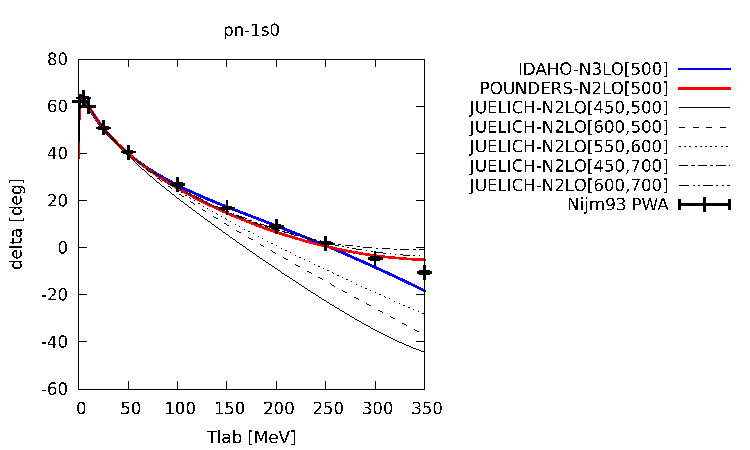
\includegraphics[width=11.0cm]{./phase-pn-1s0_IDAHO_JUELICH.pdf}
\end{center}
}

\frame
{
\frametitle{Differential cross section}
\begin{center}
\includegraphics[width=11.0cm]{./pnDSG_at_199MeV.pdf}
\end{center}
}


\end{document}

\frame
{
  \frametitle{Dramatis Personae}
\begin{center}
\begin{tabular}{llll}
\\\hline
\multicolumn{1}{c}{Baryons}&
\multicolumn{1}{c}{Mass (MeV)}&
\multicolumn{1}{c}{Mesons}&
\multicolumn{1}{c}{Mass (MeV)}
\\ \hline
$p,n$&938.926&$\pi$&138.03\\
$\Lambda$&1116.0&$\eta$&548.8\\
$\Sigma$&1197.3&$\sigma$&$\approx 550.0$\\
$\Delta$&1232.0&$\rho$&770\\
&&$\omega$&782.6\\
&&$\delta$&983.0\\
&&$K$&495.8\\
&&$K^{\star}$&895.0\\ \hline
\end{tabular}
\end{center}
}


\frame
{
\frametitle{Lagrangians}
To describe the interaction between the various baryons and mesons of the previous
table we choose the following phenomenological
lagrangians
for spin $1/2$ baryons
\[
   {\cal L}_{ps} =g^{ps}\overline{\Psi}\gamma^{5}
   \Psi\phi^{(ps)},
   \label{eq:pseudo}
\]
\[
   {\cal L}_{s} =g^{s}\overline{\Psi}\Psi\phi^{(s)},
   \label{eq:scalar}
\]
and
\[
   {\cal L}_{v} =g^{v}\overline{\Psi}\gamma_{\mu}\Psi\phi_{\mu}^{(v)}
   +g^{t}\overline{\Psi}\sigma^{\mu\nu}\Psi\left
   (\partial_{\mu}\phi_{\nu}^{(v)}
   -\partial_{\nu}\phi_{\mu}^{(v)}\right),
   \label{eq:vector}
\]
for pseudoscalar (ps), scalar (s) and vector (v) coupling, respectively.
The factors $g^{v}$ and $g^{t}$ are the vector
and tensor coupling constants, respectively.
}


\frame
{
\frametitle{Spinors for Protons and Neutrons}
For spin $1/2$ baryons, the fields $\Psi$ are expanded
in terms of the Dirac spinors (positive energy
solution shown here with $\overline{u}u=1$)
\[
   u(k\sigma)=\sqrt{\frac{E(k)+m}{2m}}
	  \left(\begin{array}{c} \chi\\ \\
	  \frac{\mbox{\boldmath $\sigma$}{\bf k}}{E(k)+m}\chi
	  \end{array}\right), 
   \label{eq:freespinor}
\]
with $\chi$ the familiar Pauli spinor and $E(k) =\sqrt{m^2 +|{\bf k}|^2}$. 
The positive energy part of the field $\Psi$ reads
\[
\Psi (x)={\displaystyle \frac{1}{(2\pi )^{3/2}}
        \sum_{{\bf k}\sigma}u(k\sigma)e^{-ikx}a_{{\bf k}\sigma}},
\]
with $a$ being a fermion annihilation operator.
}


\frame
{
\frametitle{The Classical Expression}
Expanding the free Dirac spinors
in terms of $1/m$ ($m$ is here the mass of the relevant baryon) 
results, to lowest order, in the familiar non-relativistic
expressions for baryon-baryon potentials.
The configuration space version of the interaction can be approximated as
\[
V({\bf r})= \left\{ C^0_C + C^1_C + C_\sigma 
\mbox{\boldmath $\sigma$}_1\cdot\mbox{\boldmath $\sigma$}_2
 + C_T \left( 1 + {3\over m_\alpha r} + {3\over
\left(m_\alpha r\right)^2}
\right) S_{12} (\hat r)\right.
\]
\[
+ C_{SL}\left. \left( {1\over m_\alpha r} + {1\over \left( m_\alpha r\right)^2}
\right) {\bf L}\cdot {\bf S}
\right\} \frac{e^{-m_\alpha r}}{m_\alpha r},
\]
where $m_{\alpha}$ is the mass of the relevant meson and
$S_{12}$ is the familiar tensor term.
}



\frame
{
\frametitle{OBE for Pion Exchange}
We derive now the non-relativistic one-pion exchange interaction.

Here $p_{1}$, $p_{1}'$, $p_{2}$, $p_{2}'$ and $k=p_{1}-p_{1}'$ denote 
four-momenta.  
The vertices are 
given by the pseudovector Lagrangian
\[
{\cal L}_{pv}=\frac{f_{\pi}}{m_{\pi}}\overline{\psi}\gamma_{5}\gamma_{\mu}
\psi\partial^{\mu}\phi_{\pi}.
\]
 From the Feynman diagram rules we can write the two-body interaction as  
\[
V^{pv}=\frac{f_{\pi}^{2}}{m_{\pi}^{2}}\frac{\overline{u}(p_{1}')\gamma_{5}
\gamma_{\mu}(p_{1}-p_{1}')^{\mu}u(p_{1})\overline{u}(p_{2}')\gamma_{5}
\gamma_{\nu}(p_{2}'-p_{2})^{\nu}u(p_{2})}{(p_{1}-p_{1}')^{2}-m_{\pi}^{2}}.
\]
}


\frame
{
\frametitle{OBE for Pion Exchange}
The factors $p_{1}-p_{1}'=p_{2}'-p_{2}$ are both the four-momentum of the 
exchanged meson and come from the derivative of the meson field in 
the interaction Lagrangian. 
The Dirac spinors obey 
\begin{eqnarray}
\gamma_{\mu}p^{\mu}u(p)&=&mu(p) \nonumber \\
\overline{u}(p)\gamma_{\mu}p^{\mu}&=&m\overline{u}(p). \nonumber
\end{eqnarray} 
Using these relations, together with $\{\gamma_{5},\gamma_{\mu}\}=0$, 
we find 
\begin{eqnarray}
\overline{u}(p_{1}')\gamma_{5}\gamma_{\mu}(p_{1}-p_{1}')^{\mu}u(p_{1})
&=&m\overline{u}(p_{1}')\gamma_{5}u(p_{1})+\overline{u}(p_{1}')\gamma_{\mu}
p_{1}'^{\mu}\gamma_{5}u(p_{1}) \nonumber \\
 &=&2m\overline{u}(p_{1}')\gamma_{5}u(p_{1}) \nonumber
\end{eqnarray}
and 
\[
\overline{u}(p_{2}')\gamma_{5}\gamma_{\mu}(p_{2}'-p_{2})^{\mu}=
-2m\overline{u}(p_{2}')\gamma_{5}u(p_{1}).
\]

}


\frame
{
\frametitle{OBE for Pion Exchange}
\begin{small}
We get 
\[
V^{pv}=-\frac{f_{\pi}^{2}}{m_{\pi}^{2}}4m^{2}\frac{\overline{u}(p_{1}')
\gamma_{5}u(p_{1})\overline{u}(p_{2}')\gamma_{5}u(p_{2})}{(p_{1}-p_{1}')
^{2}-m_{\pi}^{2}}.
\]
By inserting expressions for the Dirac spinors, we find
\begin{eqnarray*}
\overline{u}(p_{1}')\gamma_{5}u(p_{1})&=&\sqrt{\frac{(E_{1}'+m)(E_{1}+m)}
{4m^{2}}}\left(\begin{array}{cc}\chi^{\dagger}&-\frac{\sigma_{1}\cdot{
\bf p_{1}}}{E_{1}'
+m}\chi^{\dagger}\end{array}\right)\left(\begin{array}{cc}0&1\\1&0\end{array}
\right)\nonumber \\
 &&\times \left(\begin{array}{c}\chi\\ \frac{\sigma_{1}\cdot{\bf p_{1}}}{E_{1}+m}\chi
\end{array}\right) 
\nonumber \\
 &=&\sqrt{\frac{(E_{1}'+m)(E_{1}+m)}{4m^{2}}}\left(\frac{\sigma_{1}\cdot
{\bf p_{1}}}{E_{1}+m}-\frac{\sigma_{1}\cdot{\bf p_{1}'}}{E_{1}'+m}\right) 
\nonumber 
\end{eqnarray*}
\end{small}
}



\frame
{
\frametitle{OBE for Pion Exchange}
Similarly
\[
\overline{u}(p_{2}')\gamma_{5}u(p_{2})=\sqrt{\frac{(E_{2}'+m)(E_{2}+m)}
{4m^{2}}}\left(\frac{\sigma_{2}\cdot {\bf p}_{2}}{E_{2}+m}-
\frac{\sigma_{2}\cdot{\bf p'}_{2}}{E_{2}'+m}\right).
\]
In the CM system we have ${\bf p}_{2}=-{\bf p}_{1}$, ${\bf p'}_{2}=
-{\bf p'}_{1}$ and so $E_{2}=E_{1}$, $E_{2}'=E_{1}'$.  
We can then write down the relativistic contribution 
to the NN potential in the CM system: 
\begin{eqnarray}
V^{pv}&=&-\frac{f_{\pi}^{2}}{m_{\pi}^{2}}4m^{2}\frac{1}{(p_{1}-p_{1}')^{2}-
m_{\pi}^{2}}\frac{(E_{1}+m)(E_{1}'+m)}{4m^{2}} \nonumber \\ 
 &\times&\left(\frac{\sigma_{1}\cdot{\bf p}_{1}}{E_{1}+m}-\frac{\sigma_{1}
\cdot{\bf p'}_{1}}{E_{1}'+m}\right)\left(\frac{\sigma_{2}\cdot{\bf p}_{1}}
{E_{1}+m}-\frac{\sigma_{2}\cdot{\bf p'}_{1}}{E_{1}'+m}\right). \nonumber
\end{eqnarray}
}



\frame
{
\frametitle{OBE for Pion Exchange}
In the non-relativistic limit we have to lowest order 
\[
E_{1}=\sqrt{{\bf p}_{1}^{2}+m^{2}}\approx m \approx E_{1}'
\]
and then $(p_{1}-p_{1}')^{2}=-{\bf k}^{2}$, so we get 
for the contribution to the NN potential
\begin{eqnarray}
V^{pv}&=&-\frac{f_{\pi}^{2}}{m_{\pi}^{2}}4m^{2}\frac{1}{{\bf k}^{2}+m^{2}}
\frac{2m\cdot 2m}{4m^{2}}\frac{\sigma_{1}}{2m}\cdot({\bf p}_{1}-{\bf p'}_{1})
\frac{\sigma_{2}}{2m}\cdot ({\bf p}_{1}-{\bf p'}_{1}) \nonumber \\ 
 &=&-\frac{f_{\pi}^{2}}{m_{\pi}^{2}}
\frac{(\sigma_{1}\cdot{\bf k})(\sigma_{2}\cdot{\bf k})}{{\bf k}^{2}+m_{\pi}^{2}}.
\nonumber
\end{eqnarray}
We have omitted exchange terms and the isospin term $\mbox{\boldmath $\tau$}_1\cdot\mbox{\boldmath $\tau$}_2$.
}

\frame
{
\frametitle{OBE for Pion Exchange, from $k$-space to $r$-space}
We have
\[
V^{pv}(k)=-\frac{f_{\pi}^{2}}{m_{\pi}^{2}}
\frac{(\sigma_{1}\cdot{\bf k})(\sigma_{2}\cdot{\bf k})}{{\bf k}^{2}+m_{\pi}^{2}}.
\]
In coordinate space we have
\[
V^{pv}(r)=\int\frac{d^3k}{(2\pi)^3}e^{i{\bf kr}}V^{pv}(k)
\]
resulting in
\[
  V^{pv}(r)=-\frac{f_{\pi}^{2}}{m_{\pi}^{2}}
\sigma_{1}\cdot{\nabla}\sigma_{2}\cdot{\nabla}
\int\frac{d^3k}{(2\pi)^3}e^{i{\bf kr}}\frac{1}{{\bf k}^{2}+m_{\pi}^{2}}.
\]
We obtain
\[
V^{pv}(r)=-\frac{f_{\pi}^{2}}{m_{\pi}^{2}}\sigma_{1}\cdot{\nabla}\sigma_{2}\cdot{\nabla}\frac{e^{-m_{\pi}r}}{r}.
\]

}



\frame
{
\frametitle{OBE for Pion Exchange, really the last Step (I promise)}
Carrying out the differentation of
\[
V^{pv}(r)=-\frac{f_{\pi}^{2}}{m_{\pi}^{2}}\sigma_{1}\cdot{\nabla}\sigma_{2}\cdot{\nabla}\frac{e^{-m_{\pi}r}}{r}.
\]
we arrive at the famous one-pion exchange potential with central and tensor parts
\[
V({\bf r})= -\frac{f_{\pi}^{2}}{m_{\pi}^{2}}\left\{\mbox{\boldmath $\sigma$}_1\cdot\mbox{\boldmath $\sigma$}_2
 + C_T \left( 1 + {3\over m_\alpha r} + {3\over
\left(m_\alpha r\right)^2}
\right) S_{12} (\hat r)\right\} \frac{e^{-m_\pi r}}{m_\pi r}.
\]
For the full potential add the exchange part and the $\mbox{\boldmath $\tau$}_1\cdot\mbox{\boldmath $\tau$}_2$ term as well. (Subtle point: there is a divergence which gets cancelled by using cutoffs).
}





\frame
{
\frametitle{Other Mesons: Collecting Terms, $\sigma$}
When we perform similar non-relativistic expansions for scalar and vector mesons we obtain
for the $\sigma$ meson
\[
V^{\sigma}= g_{\sigma NN}^{2}\frac{1}{{\bf k}^{2}+m_{\sigma}^{2}}\left (-1+\frac{{\bf q}^{2}}{2M_N^2}
-\frac{{\bf k}^{2}}{8M_N^2}-\frac{{\bf LS}}{2M_N^2}\right).
\]
We note an attractive central force and spin-orbit force. This term has an intermediate range.
We have defined $1/2(p_{1}+p_{1}')={\bf q}$.
For the full potential add the exchange part and the isospin dependence as well.
}



\frame
{
\frametitle{Other Mesons: Collecting Terms, $\omega$}
We obtain
for the $\omega$ meson
\[
V^{\omega}= g_{\omega NN}^{2}\frac{1}{{\bf k}^{2}+m_{\omega}^{2}}\left (1-3\frac{{\bf LS}}{2M_N^2}\right).
\]
We note a repulsive central force and an attractive spin-orbit force. This term has  short range.
For the full potential add the exchange part and the isospin dependence as well.
}



\frame
{
\frametitle{Other Mesons: Collecting Terms, $\rho$}
Finally 
for the $\rho$ meson
\[
V^{\rho}= g_{\rho NN}^{2}\frac{{\bf k}^{2}}{{\bf k}^{2}+m_{\rho}^{2}}\left (
-2\sigma_{1}\sigma_{2}+S_{12}(\hat{k})\right)\tau_{1}\tau_{2}.
\]
We note a tensor force with sign opposite to that of the pion. This term has  short range. For the full potential add the exchange part and the isospin dependence as well.
}

\frame
{
  \frametitle{Summarizing, in terms of a boson exchange picture}
\vspace{-4.0cm}
\begin{center}
  \includegraphics[width=0.8\columnwidth]{lattice1}\\[1ex]
\end{center}
}

\frame
{
  \frametitle{Brief summary of properties of the NN interaction}
\begin{small}
{\scriptsize
    \begin{enumerate}
\item Can use a one-boson exchange picture to construct a nucleon-nucleon
interaction a la QED
\item Non-relativistic approximation yields amongst other things a spin-orbit
force which is much stronger than in atoms.
\item At large intermediate distances pion exchange dominates while 
pion resonances (other mesons) dominate at intermediate and short range 
\item  Potentials are parameterized to fit selected two-nucleon data, binding energies and scattering phase shifts.
\item Nowaydays, chiral perturbation theory gives an effective theory that allows a systematic expansion in terms of contrallable parameters. Good basis for many-body physics
    \end{enumerate}
}
\end{small}
}







 The potentials we will employ in this work, like
those of the Bonn group, are all non-local potentials defined in 
momentum space, and we will therefore not need the last equation.





\frame
{
\frametitle{How to construct the force: Partial wave expansion of the nuclear force}

\begin{small}
{\scriptsize

}
\end{small}
}


\frame
{
\frametitle{How to construct the force: Partial wave expansion of the nuclear force}

\begin{small}
{\scriptsize

}
\end{small}
}


\frame
{
\frametitle{How to construct the force: Partial wave expansion of the nuclear force}

\begin{small}
{\scriptsize

}
\end{small}
}


\frame
{
\frametitle{How to construct the force: Partial wave expansion of the nuclear force}

\begin{small}
{\scriptsize

}
\end{small}
}


\frame
{
\frametitle{How to construct the force: Partial wave expansion of the nuclear force}

\begin{small}
{\scriptsize

}
\end{small}
}
